\documentclass[10pt]{article}
\usepackage[margin=1in]{geometry}
\usepackage{color}
\definecolor{gray}{rgb}{0.7,0.7,0.7}
\usepackage{framed}
\usepackage{enumitem}
\usepackage{longtable}
\usepackage{makecell}
\usepackage[pdfborder={0 0 0},hyperfootnotes=false]{hyperref}
\usepackage[title]{appendix}
\usepackage[calc]{picture}
\usepackage{tikz}

\newlength{\bytewidth}
\newlength{\bytetotalheight}
\newlength{\bytedepth}
\newcommand*\byteboxsetup[1][2.1em]{\setlength{\bytewidth}{#1}
  \settototalheight{\bytetotalheight}{MQgjpqy}
  \settodepth{\bytedepth}{Qgjpqy}
  \addtolength{\bytetotalheight}{8pt}\addtolength{\bytedepth}{4pt}}

\newcommand*{\byteboxAux}[3]{\raisebox{-\bytedepth}
 {\begin{picture}(#1\bytewidth,\bytetotalheight)
    \multiput(0,0)(0,\bytetotalheight){2}{\line(1,0){#1\bytewidth}}
    #3
    \put(#1\bytewidth,0){\line(0,1){\bytetotalheight}}
    \put(0,\bytedepth){\makebox[#1\bytewidth][c]{#2}}
    \newcount\nticks \nticks #1\relax \advance\nticks -1\relax
    \multiput(\bytewidth,0)(\bytewidth,0){\nticks}{\line(0,1){3pt}}
  \end{picture}\strut}}

% Use as, e.g., \firstbytebox{2}{Tag}\bytebox{1}{\tt s}\bytebox{2}{int16\_t}
\newcommand*{\firstbytebox}[2]{\byteboxAux{#1}{#2}{\put(0,0){\line(0,1){\bytetotalheight}}}}
\newcommand*{\bytebox}[2]{\byteboxAux{#1}{#2}{}}

\newcommand*{\cclass}[1]{{\rm\sf :#1:}}
\newcommand*{\caret}{\textsuperscript{$\wedge$}}

\newcommand*{\memlimited}{\textcolor{gray}{\footnotesize\it limited}}

\begin{document}

\documentclass[10pt]{article}
\usepackage[margin=1in]{geometry}
\usepackage{color}
\definecolor{gray}{rgb}{0.7,0.7,0.7}
\usepackage{framed}
\usepackage{enumitem}
\usepackage{longtable}
\usepackage{makecell}
\usepackage[pdfborder={0 0 0},hyperfootnotes=false]{hyperref}
\usepackage[title]{appendix}
\usepackage[calc]{picture}
\usepackage{tikz}

\newlength{\bytewidth}
\newlength{\bytetotalheight}
\newlength{\bytedepth}
\newcommand*\byteboxsetup[1][2.1em]{\setlength{\bytewidth}{#1}
  \settototalheight{\bytetotalheight}{MQgjpqy}
  \settodepth{\bytedepth}{Qgjpqy}
  \addtolength{\bytetotalheight}{8pt}\addtolength{\bytedepth}{4pt}}

\newcommand*{\byteboxAux}[3]{\raisebox{-\bytedepth}
 {\begin{picture}(#1\bytewidth,\bytetotalheight)
    \multiput(0,0)(0,\bytetotalheight){2}{\line(1,0){#1\bytewidth}}
    #3
    \put(#1\bytewidth,0){\line(0,1){\bytetotalheight}}
    \put(0,\bytedepth){\makebox[#1\bytewidth][c]{#2}}
    \newcount\nticks \nticks #1\relax \advance\nticks -1\relax
    \multiput(\bytewidth,0)(\bytewidth,0){\nticks}{\line(0,1){3pt}}
  \end{picture}\strut}}

% Use as, e.g., \firstbytebox{2}{Tag}\bytebox{1}{\tt s}\bytebox{2}{int16\_t}
\newcommand*{\firstbytebox}[2]{\byteboxAux{#1}{#2}{\put(0,0){\line(0,1){\bytetotalheight}}}}
\newcommand*{\bytebox}[2]{\byteboxAux{#1}{#2}{}}

\newcommand*{\cclass}[1]{{\rm\sf :#1:}}
\newcommand*{\caret}{\textsuperscript{$\wedge$}}

\newcommand*{\memlimited}{\textcolor{gray}{\footnotesize\it limited}}

\begin{document}

\documentclass[10pt]{article}
\usepackage[margin=1in]{geometry}
\usepackage{color}
\definecolor{gray}{rgb}{0.7,0.7,0.7}
\usepackage{framed}
\usepackage{enumitem}
\usepackage{longtable}
\usepackage{makecell}
\usepackage[pdfborder={0 0 0},hyperfootnotes=false]{hyperref}
\usepackage[title]{appendix}
\usepackage[calc]{picture}
\usepackage{tikz}

\newlength{\bytewidth}
\newlength{\bytetotalheight}
\newlength{\bytedepth}
\newcommand*\byteboxsetup[1][2.1em]{\setlength{\bytewidth}{#1}
  \settototalheight{\bytetotalheight}{MQgjpqy}
  \settodepth{\bytedepth}{Qgjpqy}
  \addtolength{\bytetotalheight}{8pt}\addtolength{\bytedepth}{4pt}}

\newcommand*{\byteboxAux}[3]{\raisebox{-\bytedepth}
 {\begin{picture}(#1\bytewidth,\bytetotalheight)
    \multiput(0,0)(0,\bytetotalheight){2}{\line(1,0){#1\bytewidth}}
    #3
    \put(#1\bytewidth,0){\line(0,1){\bytetotalheight}}
    \put(0,\bytedepth){\makebox[#1\bytewidth][c]{#2}}
    \newcount\nticks \nticks #1\relax \advance\nticks -1\relax
    \multiput(\bytewidth,0)(\bytewidth,0){\nticks}{\line(0,1){3pt}}
  \end{picture}\strut}}

% Use as, e.g., \firstbytebox{2}{Tag}\bytebox{1}{\tt s}\bytebox{2}{int16\_t}
\newcommand*{\firstbytebox}[2]{\byteboxAux{#1}{#2}{\put(0,0){\line(0,1){\bytetotalheight}}}}
\newcommand*{\bytebox}[2]{\byteboxAux{#1}{#2}{}}

\newcommand*{\cclass}[1]{{\rm\sf :#1:}}
\newcommand*{\caret}{\textsuperscript{$\wedge$}}

\newcommand*{\memlimited}{\textcolor{gray}{\footnotesize\it limited}}

\begin{document}

\documentclass[10pt]{article}
\usepackage[margin=1in]{geometry}
\usepackage{color}
\definecolor{gray}{rgb}{0.7,0.7,0.7}
\usepackage{framed}
\usepackage{enumitem}
\usepackage{longtable}
\usepackage{makecell}
\usepackage[pdfborder={0 0 0},hyperfootnotes=false]{hyperref}
\usepackage[title]{appendix}
\usepackage[calc]{picture}
\usepackage{tikz}

\newlength{\bytewidth}
\newlength{\bytetotalheight}
\newlength{\bytedepth}
\newcommand*\byteboxsetup[1][2.1em]{\setlength{\bytewidth}{#1}
  \settototalheight{\bytetotalheight}{MQgjpqy}
  \settodepth{\bytedepth}{Qgjpqy}
  \addtolength{\bytetotalheight}{8pt}\addtolength{\bytedepth}{4pt}}

\newcommand*{\byteboxAux}[3]{\raisebox{-\bytedepth}
 {\begin{picture}(#1\bytewidth,\bytetotalheight)
    \multiput(0,0)(0,\bytetotalheight){2}{\line(1,0){#1\bytewidth}}
    #3
    \put(#1\bytewidth,0){\line(0,1){\bytetotalheight}}
    \put(0,\bytedepth){\makebox[#1\bytewidth][c]{#2}}
    \newcount\nticks \nticks #1\relax \advance\nticks -1\relax
    \multiput(\bytewidth,0)(\bytewidth,0){\nticks}{\line(0,1){3pt}}
  \end{picture}\strut}}

% Use as, e.g., \firstbytebox{2}{Tag}\bytebox{1}{\tt s}\bytebox{2}{int16\_t}
\newcommand*{\firstbytebox}[2]{\byteboxAux{#1}{#2}{\put(0,0){\line(0,1){\bytetotalheight}}}}
\newcommand*{\bytebox}[2]{\byteboxAux{#1}{#2}{}}

\newcommand*{\cclass}[1]{{\rm\sf :#1:}}
\newcommand*{\caret}{\textsuperscript{$\wedge$}}

\newcommand*{\memlimited}{\textcolor{gray}{\footnotesize\it limited}}

\begin{document}

\input{SAMv1.ver}
\title{Sequence Alignment/Map Format Specification}
\author{The SAM/BAM Format Specification Working Group}
\date{\headdate}
\maketitle
\begin{quote}\small
The master version of this document can be found at
\url{https://github.com/samtools/hts-specs}.\\
This printing is version~\commitdesc\ from that repository,
last modified on the date shown above.
\end{quote}
\vspace*{1em}


\section{The SAM Format Specification}
SAM stands for Sequence Alignment/Map format. It is a TAB-delimited text
format consisting of a header section, which is optional, and an
alignment section. If present, the header must be prior to the
alignments. Header lines start with `{\tt @}', while alignment lines do
not. Each alignment line has 11 mandatory fields for essential alignment
information such as mapping position, and variable number of optional
fields for flexible or aligner specific information.

This specification is for version 1.6 of the SAM and BAM formats.  Each SAM and
BAM file may optionally specify the version being used via the
{\tt @HD VN} tag. For full version history see Appendix~\ref{sec:history}. 

Unless explicitly specified elsewhere, all fields are encoded using 7-bit US-ASCII \footnote{Charset ANSI\_X3.4-1968 as defined in RFC1345.} in using the POSIX / C locale.
Regular expressions listed use the POSIX / IEEE Std 1003.1 extended syntax.

\subsection{An example}\label{sec:example}
Suppose we have the following alignment with bases in lowercase
clipped from the alignment. Read {\tt r001/1} and {\tt r001/2}
constitute a read pair; {\tt r003} is a chimeric read; {\tt r004}
represents a split alignment.

\begin{framed}\small
\begin{verbatim}
Coor     12345678901234  5678901234567890123456789012345
ref      AGCATGTTAGATAA**GATAGCTGTGCTAGTAGGCAGTCAGCGCCAT

+r001/1        TTAGATAAAGGATA*CTG
+r002         aaaAGATAA*GGATA
+r003       gcctaAGCTAA
+r004                     ATAGCT..............TCAGC
-r003                            ttagctTAGGC
-r001/2                                        CAGCGGCAT
\end{verbatim}
\end{framed}
The corresponding SAM format is:\footnote{The values in the
{\sf FLAG} column correspond to bitwise flags as follows:
99 = 0x63: first\slash next is reverse-complemented\slash
properly aligned\slash multiple segments;
0: no flags set, thus a mapped single segment;
2064 = 0x810: supplementary\slash reverse-complemented;
147 = 0x93: last (second of a pair)\slash reverse-complemented\slash
properly aligned\slash multiple segments.}
\begin{framed}\small
\begin{verbatim}
@HD VN:1.6 SO:coordinate
@SQ SN:ref LN:45
r001   99 ref  7 30 8M2I4M1D3M = 37  39 TTAGATAAAGGATACTG *
r002    0 ref  9 30 3S6M1P1I4M *  0   0 AAAAGATAAGGATA    *
r003    0 ref  9 30 5S6M       *  0   0 GCCTAAGCTAA       * SA:Z:ref,29,-,6H5M,17,0;
r004    0 ref 16 30 6M14N5M    *  0   0 ATAGCTTCAGC       *
r003 2064 ref 29 17 6H5M       *  0   0 TAGGC             * SA:Z:ref,9,+,5S6M,30,1;
r001  147 ref 37 30 9M         =  7 -39 CAGCGGCAT         * NM:i:1
\end{verbatim}
\end{framed}

\subsection{Terminologies and Concepts}

\begin{description}
\item[Template] A DNA/RNA sequence part of which is sequenced on a
  sequencing machine or assembled from raw sequences.

\item[Segment] A contiguous sequence or subsequence.

\item[Read] A raw sequence that comes off a sequencing machine. A read
  may consist of multiple segments. For sequencing data, reads are indexed by
  the order in which they are sequenced.

\item[Linear alignment]
  An alignment of a read to a single reference sequence that may include
  insertions, deletions, skips and clipping, but may not include direction
  changes (i.e., one portion of the alignment on forward strand and another
  portion of alignment on reverse strand). A linear alignment can be
  represented in a single SAM record.
%  A alignment of a read to a single locus on the reference, where the
%  alignment may have short insertions/deletions but does not have long gaps
%  (e.g., due to introns or structural variation).

\item[Chimeric alignment]
  An alignment of a read that cannot be represented as a linear alignment. A
  chimeric alignment is represented as a set of linear alignments that do not
  have large overlaps.  Typically, one of the linear alignments in a chimeric
  alignment is considered the ``representative'' alignment, and the others are
  called ``supplementary'' and are distinguished by the supplementary alignment
  flag.  All the SAM records in a chimeric alignment have the same {\sf QNAME}
  and the same values for 0x40 and 0x80 flags (see Section~\ref{sec:alnrecord}).
  The decision regarding which linear alignment is representative is arbitrary.

\item[Read alignment]
  A linear alignment or a chimeric alignment that is the complete
  representation of the alignment of the read.

\item[Multiple mapping]
  The correct placement of a read may be ambiguous, e.g., due to repeats.  In
  this case, there may be multiple read alignments for the same read.  One of
  these alignments is considered primary.  All the other alignments have the
  secondary alignment flag set in the SAM records that represent them.  All the
  SAM records have the same {\sf QNAME} and the same values for 0x40 and 0x80
  flags.  Typically the alignment designated primary is the best alignment, but
  the decision may be arbitrary.\footnotemark

\item[1-based coordinate system] A coordinate system where the first
  base of a sequence is one. In this coordinate system, a region is
  specified by a closed interval. For example, the region between the
  3rd and the 7th bases inclusive is $[3,7]$. The SAM, VCF, GFF and Wiggle
  formats are using the 1-based coordinate system.

\item[0-based coordinate system] A coordinate system where the first
  base of a sequence is zero. In this coordinate system, a region is
  specified by a half-closed-half-open interval. For example, the region
  between the 3rd and the 7th bases inclusive is $[2,7)$. The BAM, BCFv2, BED,
  and PSL formats are using the 0-based coordinate system.

\item[Phred scale] Given a probability $0<p\le 1$, the phred scale of $p$
  equals $-10\log_{10}p$, rounded to the closest integer.

\end{description}

\footnotetext{Chimeric alignments are primarily caused by structural
variations, gene fusions, misassemblies, RNA-seq or experimental protocols.
They are more frequent given longer reads.
For a chimeric alignment, the linear alignments constituting the alignment are largely
non-overlapping; each linear alignment may have high mapping quality and is
informative in SNP/INDEL calling. In contrast, multiple mappings are caused primarily by repeats.  They are less frequent
given longer reads. If a read has multiple mappings, all these mappings are
almost entirely overlapping with each other; except the single-best optimal
mapping, all the other mappings get mapping quality $<$Q3
and are ignored by most SNP/INDEL callers.}

\subsubsection{Character set restrictions}\label{sec:charset}

Reference sequence names, CIGAR strings, and several other field types are used as values or parts of values of other fields in SAM and related formats such as VCF.
To ensure that these other fields' representations are unambiguous, these field types disallow particular delimiter characters.

Query or read names may contain any printable ASCII characters in the range \verb"[!-~]" apart from `\verb"@"', so that SAM alignment lines can be easily distinguished from header lines.
(They are also limited in length.)

Reference sequence names may contain any printable ASCII characters in the range {\tt [!-\verb:~:]} apart from backslashes, commas, quotation marks, and brackets---i.e., apart from `{\tt \verb:\:\,,\,"`'\,()\,[]\,\verb:{}:\,<>}'---and may not start with `{\tt *}' or `{\tt =}'.%
\footnote{Characters that are \emph{not} disallowed include `{\tt |}', which historically appeared in reference names derived from NCBI FASTA files, and `{\tt :}', which appears in HLA allele names.
Appendix~\ref{sec:parse-region} describes approaches for parsing \emph{name}{\tt [:}\emph{begin}{\tt -}\emph{end}{\tt ]} region notation unambiguously even though \emph{name} may itself contain colons.}

Thus they match the following regular expression:
\begin{center}
{\tt [\verb"0-9A-Za-z!#$%&+./:;?@^_|~-"][\verb"0-9A-Za-z!#$%&*+./:;=?@^_|~-"]*}
\end{center}

% Pedantically this should be [[:rname:]^*=][[:rname:]]*, but we take advantage
% of POSIX (Issue 7) section 9.3.5/8 to elide the excess brackets for clarity.
\newcommand*{\rnameRegexp}{[\cclass{rname}\caret*=][\cclass{rname}]*}

\noindent
For clarity, elsewhere in this specification we write this set of allowed characters as a character class~{\tt [\cclass{rname}]} and extend the POSIX regular expression notation to use {\tt\caret *=} to indicate the omission of `{\tt *}' and `{\tt =}' from the character class.
Thus this regular expression can be written more clearly as {\tt\rnameRegexp}.

\subsection{The header section}
Each header line begins with the character `{\tt @}' followed by
one of the two-letter header record type codes defined in this section.
In the header, each line is TAB-delimited and, apart from {\tt @CO} lines,
each data field follows a format `{\tt TAG:VALUE}' where {\tt TAG}
is a two-character string that defines the format and content of {\tt VALUE}.
Thus header lines match {\tt
  /\char94@(HD|SQ|RG|PG)(\char92t[A-Za-z][A-Za-z0-9]:[
  -\char126]+)+\$/} or {\tt /\char94@CO\char92t.*/}.

The following table describes the header record types that may be used
and their predefined tags.
Tags listed with `*' are required; e.g., every {\tt @SQ} header line must
have {\tt SN} and {\tt LN} fields.
As with alignment optional fields (see Section~\ref{sec:alnaux}),
you can freely add new tags for further data fields.
Tags containing lowercase letters are reserved for local use and will not be
formally defined in any future version of this specification.%
\footnote{Best practice is to use lowercase tags while designing and
experimenting with new data field tags or for fields of local interest only.
For new tags that are of general interest, raise an
\href{https://github.com/samtools/hts-specs/issues}{{\tt hts-specs} issue}
or email {\tt samtools-devel@lists.sourceforge.net} to have an uppercase
equivalent added to the specification.
This way collisions of the same uppercase tag being used with different
meanings can be avoided.}

\begin{center}
\small
\begin{longtable}{|l|l|p{13.5cm}|}
  \cline{1-3}
  \multicolumn{2}{|l|}{\bf Tag} & {\bf Description} \\
  \cline{1-3}
  \endfirsthead
  \cline{1-3}
  \endhead
  \multicolumn{2}{|l}{\tt @HD} & File-level metadata. Optional. If present, there must be only one {\tt @HD} line and it must be the first line of the file. \\\cline{2-3}
  & {\tt VN}* & Format version. \emph{Accepted format}: {\tt /\char94[0-9]+\char92.[0-9]+\$/}.\\\cline{2-3}
  & {\tt SO} & Sorting order of alignments. \emph{Valid values}: {\tt unknown} (default), {\tt
    unsorted}, {\tt queryname} and {\tt coordinate}. For coordinate sort, the major sort
  key is the {\sf RNAME} field, with order defined by the order of {\tt @SQ} lines in the header.  The
  minor sort key is the {\sf POS} field.  For alignments with equal {\sf RNAME} and {\sf POS}, order is
  arbitrary.  All alignments with `{\tt *}' in {\sf RNAME} field follow alignments with some other
  value but otherwise are in arbitrary order.
  For queryname sort, no explicit requirement is made regarding the ordering other than that it be applied consistently throughout the entire file.%
  \footnote{It is known that widely used software libraries have differing definitions of the queryname sort order, meaning care should be taken when operating on multiple files of varying provenance.
  Tools may wish to use the sub-sort field to explicitly distinguish between natural and lexicographical ordering.  See Section~\ref{sec:sub-sort}.}\\\cline{2-3}
  & {\tt GO} & Grouping of alignments, indicating that similar alignment records
    are grouped together but the file is not necessarily sorted overall.
    \emph{Valid values}: {\tt none} (default), {\tt query} (alignments are
    grouped by {\sf QNAME}), and {\tt reference} (alignments are grouped by
    {\sf RNAME}/{\sf POS}).\\\cline{1-3}
  & {\tt SS} & Sub-sorting order of alignments. Valid values are of the form \emph{sort-order}{\tt :}\emph{sub-sort}, where \emph{sort-order} is the same value stored in the {\tt SO} tag and \emph{sub-sort} is an implementation-dependent colon-separated string further describing the sort order, but with some predefined terms defined in Section~\ref{sec:sub-sort}.
    For example, if an algorithm relies on a {\tt coordinate} sort that, at each coordinate, is further sorted by query name then the header could contain {\tt @HD SO:coordinate SS:coordinate:queryname}.%
\footnote{The repetition of \emph{sort-order} enables a limited form of validation.
For example, {\tt @HD SO:queryname SS:coordinate:TLEN} would indicate that the data has been re-sorted (by query name) by a non-{\tt SS}-aware tool and the {\tt SS} field should be ignored.}
    If the primary sort is not one of the predefined primary sort orders, then {\tt unsorted} should be used and the subsort is effectively the major sort.
    For example, if sorted by an auxiliary tag {\tt MI} then by coordinate then the header could contain {\tt @HD SO:unsorted SS:unsorted:MI:coordinate}.
    \newline
    \emph{Regular expression}: {\tt (coordinate|queryname|unsorted)(:[\verb"A-Za-z0-9_-"]+)+}\\\cline{1-3}
  \multicolumn{2}{|l}{\tt @SQ} & Reference sequence dictionary. The order of {\tt @SQ} lines defines the alignment sorting order.\\\cline{2-3}
  & {\tt SN}* & Reference sequence name.
The {\tt SN} tags and all individual {\tt AN} names in all {\tt @SQ} lines
must be distinct.
  The value of this field is used in the
  alignment records in {\sf RNAME} and {\sf RNEXT} fields. Regular expression: {\tt\rnameRegexp}\\\cline{2-3}
  & {\tt LN}* & Reference sequence length. \emph{Range}: $[1,\,2^{31}-1]$\\\cline{2-3}
  & {\tt AH} & Indicates that this sequence is an alternate locus.%
\footnote{See \url{https://www.ncbi.nlm.nih.gov/grc/help/definitions} for descriptions of \emph{alternate locus} and \emph{primary assembly}.}
  The value is the locus in the primary assembly for which this sequence is an alternative, in the format `\emph{chr}{\tt :}\emph{start}{\tt -}\emph{end}', `\emph{chr}' (if known), or `{\tt *}' (if unknown), where `\emph{chr}' is a sequence in the primary assembly.
  Must not be present on sequences in the primary assembly.\\\cline{2-3}
  & {\tt AN} & Alternative reference sequence names.
A comma-separated list of alternative names that tools may use when referring
to this reference sequence.%
\footnote{For example, given `{\tt @SQ SN:MT AN:chrMT,M,chrM LN:16569 TP:circular}',
tools can ensure that a user's request for any of `MT', `chrMT', `M',
or~`chrM' succeeds and refers to the same sequence.}
These alternative names are not used elsewhere within the SAM file;
in particular, they must not appear in alignment records' {\sf RNAME}
or~{\sf RNEXT} fields.
\emph{Regular expression}: \emph{name}{\tt (,}\emph{name}{\tt )*}
where \emph{name} is {\tt\rnameRegexp}\\\cline{2-3}
  & {\tt AS} & Genome assembly identifier. \\\cline{2-3}
  & {\tt DS} & Description.  UTF-8 encoding may be used.\\\cline{2-3}
  & {\tt M5} & MD5 checksum of the sequence.  See Section~\ref{sec:ref-md5}\\\cline{2-3}
  & {\tt SP} & Species.\\\cline{2-3}
  & {\tt TP} & Molecule topology. \emph{Valid values}: {\tt linear} (default) and {\tt circular}.%
\footnote{The previous footnote's example identifies MT as a circular chromosome.
The {\tt TP} field is often omitted, which implies linear.}\\\cline{2-3}
  & {\tt UR} & URI of the sequence.  This value may start with one of the standard
  protocols, e.g., `{\tt http:}' or `{\tt ftp:}'.  If it does not start with one of these protocols, it is assumed to be a file-system path.\\\cline{1-3}
  \multicolumn{2}{|l}{\tt @RG} & Read group. Unordered multiple {\tt @RG} lines are allowed.\\\cline{2-3}
  & {\tt ID}* & Read group identifier. Each {\tt @RG} line must have a unique {\tt ID}. The value of {\tt ID}
  is used in the RG tags of alignment records. Must be unique among all read groups in header section.  Read group IDs may be modified when merging SAM files in order to handle collisions.\\\cline{2-3}
  & {\tt BC} & Barcode sequence identifying the sample or library.
  This value is the expected barcode bases as read by the sequencing machine in the absence of errors.
  If there are several barcodes for the sample/library (e.g., one on each end of the template), the recommended implementation concatenates all the barcodes separating them with hyphens (`{\tt -}').\\\cline{2-3}
  & {\tt CN} & Name of sequencing center producing the read.\\\cline{2-3}
  & {\tt DS} & Description.  UTF-8 encoding may be used.\\\cline{2-3}
  & {\tt DT} & Date the run was produced (ISO8601 date or date/time).\\\cline{2-3}
  & {\tt FO} & Flow order. The array of nucleotide bases that correspond to the nucleotides used for each flow of each read.
  	Multi-base flows are encoded in IUPAC format, and non-nucleotide flows by various other characters. \emph{Format}: {\tt /\char92*|[ACMGRSVTWYHKDBN]+/}\\\cline{2-3}
  & {\tt KS} & The array of nucleotide bases that correspond to the key sequence of each read.\\\cline{2-3}
  & {\tt LB} & Library.\\\cline{2-3}
  & {\tt PG} & Programs used for processing the read group.\\\cline{2-3}
  & {\tt PI} & Predicted median insert size.\\\cline{2-3}
  & {\tt PL} & Platform/technology used to produce the reads. \emph{Valid values}:
  {\tt CAPILLARY}, {\tt DNBSEQ} (MGI/BGI), {\tt HELICOS}, {\tt ILLUMINA}, {\tt IONTORRENT}, {\tt LS454}, {\tt ONT} (Oxford Nanopore), {\tt PACBIO} (Pacific Biotechnology), and {\tt SOLID}.
  This field should be omitted when the technology is not in this list (though the {\tt PM} field may still be present in this case) or is unknown.\\\cline{2-3}
  & {\tt PM} & Platform model. Free-form text providing further details of the platform/technology used.\\\cline{2-3}
  & {\tt PU} & Platform unit (e.g., flowcell-barcode.lane for Illumina or slide for SOLiD). Unique identifier.\\\cline{2-3}
  & {\tt SM} & Sample. Use pool name where a pool is being sequenced.\\\cline{1-3}
  \multicolumn{2}{|l}{\tt @PG} & Program. \\\cline{2-3}
  & {\tt ID}* & Program record identifier. Each {\tt @PG} line must have a unique {\tt ID}.
  	The value of {\tt ID} is used in the alignment {\tt PG} tag and {\tt PP} tags of other {\tt @PG} lines.
	{\tt PG} IDs may be modified when merging SAM files in order to handle collisions.\\\cline{2-3}
  & {\tt PN} & Program name \\\cline{2-3}
  & {\tt CL} & Command line.  UTF-8 encoding may be used. \\\cline{2-3}
  & {\tt PP} & Previous {\tt @PG-ID}. Must match another {\tt @PG} header's {\tt ID} tag.
  	{\tt @PG} records may be chained using {\tt PP} tag, with the last record in the chain
	having no {\tt PP} tag. This chain defines the order of programs that have been applied to the alignment.
	{\tt PP} values may be modified when merging SAM files in order to handle collisions of {\tt PG} {\tt ID}s.
	The first {\tt PG} record in a chain (i.e., the one referred to by the {\tt PG} tag in a SAM record)
	describes the most recent program that operated on the SAM record.
	The next {\tt PG} record in the chain describes the next most recent program that
        operated on the SAM record. The {\tt PG} {\tt ID} on a SAM record is not required
        to refer to the newest {\tt PG} record in a chain.  It may refer to any {\tt PG}
        record in a chain, implying that the SAM record has been operated on by the
        program in that {\tt PG} record, and the program(s) referred to via the {\tt PP} tag. \\\cline{2-3}
  & {\tt DS} & Description.  UTF-8 encoding may be used.\\\cline{2-3}
  & {\tt VN} & Program version \\\cline{1-3}
  \multicolumn{2}{|l}{\tt @CO} & One-line text comment. Unordered multiple {\tt @CO} lines are allowed. UTF-8 encoding may be used.\\
  \cline{1-3}
\end{longtable}
\end{center}

\subsubsection{Defined sub-sort terms}\label{sec:sub-sort}

While the {\tt SS} sub-sort field allows implementation-defined keywords, some terms are predefined with specific meanings.

\begin{description}
\item[lexicographical] sort order is defined as a character-based dictionary sort with the character order as defined by the POSIX C locale.
  For example ``abc'', ``abc17'', ``abc5'', ``abc59'' and ``abcd'' are in lexicographical order.

\item[natural] sort order is similar to lexicographical order except that runs of adjacent digits are considered to be numbers embedded within the text string, ordered numerically when compared to each other and ordered as single digits when compared to the surrounding non-digit characters.
Runs that differ only in the number of leading zeros (thus are numerically tied) are ordered by more-zeros coming before fewer-zeros.
The characters `\texttt{-}' and `\texttt{.}' are considered as ordinary characters, so apparently negative or fractional values are not treated as part of an embedded number.
  For example, ``abc'', ``abc+5'', ``abc-5'', ``abc.d'', ``abc03'', ``abc5'', ``abc008'', ``abc08'', ``abc8'', ``abc17'', ``abc17.+'', ``abc17.2'', ``abc17.d'', ``abc59'' and ``abcd'' are in natural order.

\item[umi] is a lexicographical sort by the UMI tag.
  The {\tt MI} tag should be used for comparing UMIs. The RX tag may be used in its absence but is not guaranteed to be unique across multiple libraries.

\end{description}

\subsubsection{Reference MD5 calculation}\label{sec:ref-md5}
The {\tt M5} tag on {\tt @SQ} lines allows reference sequences to be uniquely identified through the MD5 digest of the sequence itself.
As the digest is based on the sequence and nothing else, it can help resolve ambiguities with reference naming.
For example, it allows a quick way of checking that references named `1', `Chr1' and `chr1' in different files are in fact the same.

The reference sequence must be in the 7-bit US-ASCII character set.
All valid reference bases can be represented in this set, and it avoids the problem of determining exactly which 8-bit representation may have been used.
Padding characters (See Section~\ref{sec:padded-sam}) must be represented only using the `*' character. 

The digest is calculated as follows:
\begin{itemize}
\item All characters outside of the inclusive range 33 (`\char33') to 126 (`\char126') are stripped out.
This removes all unprintable and whitespace characters including spaces and new lines.
Everything else is retained, even if not a legal nucleotide code.
\item All lowercase characters are converted to uppercase.
This operation is equivalent to calling \href{http://pubs.opengroup.org/onlinepubs/9699919799/functions/toupper.html}{\sl toupper()} on characters in the \href{http://pubs.opengroup.org/onlinepubs/9699919799/basedefs/V1\_chap07.html\#tag\_07\_02}{\sl POSIX locale}.
\item The MD5 digest is calculated as described in \href{https://tools.ietf.org/html/rfc1321}{\sl RFC 1321} and presented as a 32 character lowercase hexadecimal number.
\end{itemize}

As an example, if the reference contains the following characters (including spaces):
\begin{verbatim}
ACGT ACGT ACGT
acgt acgt acgt
... 12345 !!!
\end{verbatim}
then the digest is that of the string {\tt ACGTACGTACGTACGTACGTACGT...12345!!!}
and the resulting tag would be {\tt M5:dfabdbb36e239a6da88957841f32b8e4}.

In padded SAM files, the padding bases should be inserted into the reference as `*' characters.
Taking the example in Section~\ref{sec:padded-sam}, the padded version of the reference is
\begin{verbatim}
AGCATGTTAGATAA**GATAGCTGTGCTAGTAGGCAGTCAGCGCCAT
\end{verbatim}
and the corresponding tag is {\tt M5:caad65b937c4bc0b33c08f62a9fb5411}.

\subsection{The alignment section: mandatory fields}\label{sec:alnrecord}
In the SAM format, each alignment line typically represents the linear alignment of a segment.
Each line consists of 11~or more TAB-separated fields.
The first eleven fields are always present and in the order shown below; if the information represented by any of these fields is unavailable, that field's value will be a placeholder, either~`{\tt 0}' or~`{\tt *}' as determined by the field's type.
The following table gives an overview of these mandatory fields in the SAM format:
\begin{center}
\small
\begin{tabular}{rllll}
  \hline
  {\bf Col} & {\bf Field} & {\bf Type} & {\bf Regexp/Range} & {\bf Brief description} \\
  \hline
  1 & {\sf QNAME} & String & \verb:[!-?A-~]{1,254}: & Query template NAME\\
  2 & {\sf FLAG} & Int & $[0,\,2^{16}-1]$ & bitwise FLAG \\
  3 & {\sf RNAME} & String & {\tt \verb"\*"|\rnameRegexp} & Reference sequence NAME\footnotemark \\
  4 & {\sf POS} & Int & $[0,\,2^{31}-1]$ & 1-based leftmost mapping POSition \\
  5 & {\sf MAPQ} & Int & $[0,\,2^8-1]$ & MAPping Quality \\
  6 & {\sf CIGAR} & String & {\tt \char92*|([0-9]+[MIDNSHPX=])+} & CIGAR string \\
  7 & {\sf RNEXT} & String & {\tt \verb"\*"|=|\rnameRegexp} & Reference name of the mate/next read \\
  8 & {\sf PNEXT} & Int & $[0,\,2^{31}-1]$ & Position of the mate/next read \\
  9 & {\sf TLEN} & Int & $[-2^{31}+1,\,2^{31}-1]$ & observed Template LENgth \\
  10 & {\sf SEQ} & String & {\tt \char92*|[A-Za-z=.]+} & segment SEQuence\\
  11 & {\sf QUAL} & String & {\tt [!-\char126]+} & ASCII of Phred-scaled base QUALity+33 \\
  \hline
\end{tabular}
\end{center}

\footnotetext{Reference sequence names may contain any printable ASCII characters with the exception of certain punctuation characters, and may not start with `{\tt *}' or `{\tt =}'.
See Section~\ref{sec:charset} for details and an explanation of the {\tt [\cclass{rname}]} notation.}

\noindent
All mapped segments in alignment lines are represented on the forward genomic strand.
For segments that have been mapped to the reverse strand, the recorded {\sf SEQ} is reverse complemented from the original unmapped sequence and {\sf CIGAR}, {\sf QUAL}, and strand-sensitive optional fields are reversed and thus recorded consistently with the sequence bases as represented.

\begin{enumerate}
\item {\sf QNAME}: Query template NAME. Reads/segments having identical {\sf QNAME}
	are regarded to come from the same template. A {\sf QNAME} `{\tt *}'
	indicates the information is unavailable.  In a SAM file, a read may occupy
	multiple alignment lines, when its alignment is chimeric or when multiple
	mappings are given.
\item {\sf FLAG}: Combination of bitwise FLAGs.\footnote{The manipulation of
bitwise flags is described at \href{http://en.wikipedia.org/wiki/Flag\_field}
{Wikipedia (see ``Flag field'')} and elsewhere.}
Each bit is explained in the following table:
  \begin{center}\small
  \begin{tabular}{rrl}
  \hline
  \multicolumn{2}{c}{Bit} & Description\\
  \hline
    1 &    0x1 & template having multiple segments in sequencing \\
    2 &    0x2 & each segment properly aligned according to the aligner \\
    4 &    0x4 & segment unmapped \\
    8 &    0x8 & next segment in the template unmapped \\
   16 &   0x10 & {\sf SEQ} being reverse complemented \\
   32 &   0x20 & {\sf SEQ} of the next segment in the template being reverse complemented \\
   64 &   0x40 & the first segment in the template \\
  128 &   0x80 & the last segment in the template \\
  256 &  0x100 & secondary alignment \\
  512 &  0x200 & not passing filters, such as platform/vendor quality controls \\
 1024 &  0x400 & PCR or optical duplicate \\
 2048 &  0x800 & supplementary alignment \\
  \hline
  \end{tabular}
  \end{center}
  \begin{itemize}
  \item For each read/contig in a SAM file, it is required that one and only
	one line associated with the read satisfies \mbox{`{\sf FLAG} {\tt \& 0x900
	== 0}'}. This line is called the \emph{primary line} of the read.
  \item Bit 0x100 marks the alignment not to be used in certain analyses
    when the tools in use are aware of this bit. It is typically used to
	flag alternative mappings when multiple mappings are presented in a SAM.
  \item Bit 0x800 indicates that the corresponding alignment line is part of
    a chimeric alignment. A line flagged with 0x800 is called as a \emph{supplementary line}.
  \item Bit 0x4 is the only reliable place to tell whether the read
    is unmapped. If 0x4 is set, no assumptions can be made about {\sf
      RNAME}, {\sf POS}, {\sf CIGAR}, {\sf MAPQ}, and bits 0x2, 0x100,
    and 0x800.
  \item Bit 0x10 indicates whether {\sf SEQ} has been reverse complemented
    and {\sf QUAL} reversed.
    When bit~0x4 is unset, this corresponds to the strand to which the
    segment has been mapped: bit~0x10 unset indicates the forward strand,
    while set indicates the reverse strand.
    When 0x4 is set, this indicates whether the unmapped read is stored
    in its original orientation as it came off the sequencing machine.
  \item Bits 0x40 and 0x80 reflect the read ordering within each template
    inherent in the sequencing technology used.\footnote{For example,
    in Illumina paired-end sequencing, {\sf first}~(0x40) corresponds to
    the R1~`forward' read and {\sf last}~(0x80) to the R2~`reverse' read.
    (Despite the terminology, this is unrelated to the segments' orientations
    when they are mapped: either, neither, or both may have their
    {\sf reverse} flag bits~(0x10) set after mapping.)}
    If 0x40 and 0x80 are both set, the read is part of a linear
    template, but it is neither the first nor the last read. If both
    0x40 and 0x80 are unset, the index of the read in the template
    is unknown. This may happen for a non-linear template or when this
    information is lost during data processing.
  \item If 0x1 is unset, no assumptions can be made about 0x2, 0x8,
    0x20, 0x40 and 0x80.
  \item Bits that are not listed in the table are reserved for future use.
    They should not be set when writing and should be ignored on reading
    by current software.
  \end{itemize}
\item {\sf RNAME}: Reference sequence NAME of the alignment. If {\tt
    @SQ} header lines are present, {\sf RNAME} (if not `*') must be
  present in one of the {\tt SQ-SN} tag. An unmapped segment without
  coordinate has a `*' at this field. However, an unmapped segment may
  also have an ordinary coordinate such that it can be placed at a
  desired position after sorting. If {\sf RNAME} is `*', no assumptions
  can be made about {\sf POS} and {\sf CIGAR}.
\item {\sf POS}: 1-based leftmost mapping POSition of the first {\sf
    CIGAR} operation that ``consumes'' a reference base (see table below).
    The first base in a reference sequence has coordinate 1. {\sf
    POS} is set as 0 for an unmapped read without coordinate. If {\sf
    POS} is 0, no assumptions can be made about {\sf RNAME} and {\sf
    CIGAR}.
\item {\sf MAPQ}: MAPping Quality. It equals
  $-10\log_{10}\Pr\{\mbox{mapping position is wrong}\}$, rounded to the
  nearest integer. A value 255 indicates that the mapping quality is not
  available.
\item {\sf CIGAR}: CIGAR string. The CIGAR operations are given in the
  following table (set `*' if unavailable):
  \begin{center}\small
  \begin{tabular}{cclcc}
  \hline
  Op & BAM & Description & \makecell{Consumes \\ query} & \makecell{Consumes \\ reference}\\
  \hline
  {\tt M} & 0 & alignment match (can be a sequence match or mismatch)       & yes & yes \\
  {\tt I} & 1 & insertion to the reference                                  & yes & no  \\
  {\tt D} & 2 & deletion from the reference                                 & no  & yes \\
  {\tt N} & 3 & skipped region from the reference                           & no  & yes \\
  {\tt S} & 4 & soft clipping (clipped sequences present in {\sf SEQ})      & yes & no  \\
  {\tt H} & 5 & hard clipping (clipped sequences NOT present in {\sf SEQ})  & no  & no  \\
  {\tt P} & 6 & padding (silent deletion from padded reference)             & no  & no  \\
  {\tt =} & 7 & sequence match                                              & yes & yes \\
  {\tt X} & 8 & sequence mismatch                                           & yes & yes \\
  \hline
  \end{tabular}
  \end{center}
  \begin{itemize}
  \item ``Consumes query'' and ``consumes reference'' indicate
    whether the CIGAR operation causes the alignment to step along the
    query sequence and the reference sequence respectively.
  \item {\tt H} can only be present as the first and/or last operation.
  \item {\tt S} may only have {\tt H} operations between them and the
    ends of the {\sf CIGAR} string.
  \item For mRNA-to-genome alignment, an {\tt N} operation represents an
    intron. For other types of alignments, the interpretation of {\tt N}
    is not defined.
  \item Sum of lengths of the {\tt M/I/S/=/X} operations shall equal
    the length of {\sf SEQ}.
  \end{itemize}
\item {\sf RNEXT}: Reference sequence name of the primary alignment of the NEXT read in the
  template. For the last read, the next read is the first
  read in the template. If {\tt @SQ} header lines are present, {\sf
    RNEXT} (if not `*' or `=') must be present in one of the {\tt SQ-SN}
  tag. This field is set as `*' when the information is unavailable, and
  set as `=' if {\sf RNEXT} is identical {\sf RNAME}. If not `=' and the
  next read in the template has one primary mapping (see also bit
  0x100 in {\sf FLAG}), this field is identical to {\sf RNAME} at the primary line of the
  next read.  If {\sf
    RNEXT} is `*', no assumptions can be made on {\sf PNEXT} and bit
  0x20.
\item {\sf PNEXT}: 1-based Position of the primary alignment of the NEXT read in the template. Set as
  0 when the information is unavailable. This field equals {\sf POS} at the primary line of
  the next read. If {\sf PNEXT} is 0, no assumptions can be made on
  {\sf RNEXT} and bit 0x20.
\item {\sf TLEN}: signed observed Template LENgth. If all segments are
  mapped to the same reference sequence, the absolute value of TLEN
  equals the distance between the mapped end of the template and the
  mapped start of the template, inclusively (i.e., $\mbox{end}-\mbox{start}+1$).%
  \footnote{Thus a segment
    aligning in the forward direction at base 100 for length 50 and a
    segment aligning in the reverse direction at base 200 for length
    50 indicate the template covers bases 100 to 249 and has length
    150.}
  Note that \textit{mapped base} is defined to be one that aligns to the
  reference as described by CIGAR, hence excludes soft-clipped bases.
  The TLEN field is positive for the leftmost segment of the template,
  negative for the rightmost, and the sign for any middle segment is
  undefined.  If segments cover the same coordinates then the choice
  of which is leftmost and rightmost is arbitrary, but the two ends
  must still have differing signs.
  It is set as 0 for a single-segment template or when the
  information is unavailable (e.g., when the first or last segment
  of a multi-segment template is unmapped or when the two are mapped
  to different reference sequences).

% If future updates cause this footnote to spill over the page boundary
% try e.g. \enlargethispage{-10em} to adjust where this page ends.
  The intention of this field is to indicate where the other end of
  the template has been aligned without needing to read the remainder
  of the SAM file.  Unfortunately there has been no
  clear consensus on the definitions of the template mapped start
  and end.  Thus the exact definitions are implementation-defined.%
\footnote{The earliest versions of this specification used $5'$ to
  $5'$ (in original orientation, TLEN\#1; dashed parts of the reads
  indicate soft-clipped bases) while later ones used leftmost to
  rightmost mapped base (TLEN\#2).  Note: these two definitions agree in most
  alignments, but differ in the case of overlaps where the first
  segment aligns beyond the start of the last segment.

\begin{center}
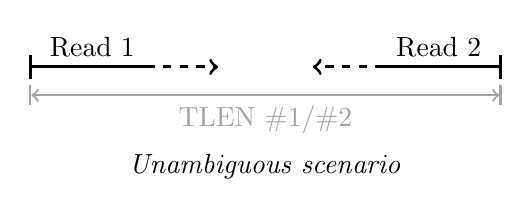
\begin{tikzpicture}[
    thick, xscale=2, yscale=1.8,
    read/.style={line width=0.4mm},
]
\draw[|-, read] (0,0)   -- (0.8,0)  node[midway, above] {Read 1};
\draw[->, read, dashed] (0.85,0) -- (1.2,0);
\draw[|-, read] (3,0) -- (2.2,0) node[midway, above] {Read 2};
\draw[->, read, dashed] (2.25,0) -- (1.8,0);
\draw[|<->|,gray!120]     (0,-.2) -- +(3,0) node[midway, below] {TLEN \#1/\#2};
\node at (1.5,-0.7) {\textit{Unambiguous scenario}};
\end{tikzpicture}
\hspace{3cm}% No space means side by side
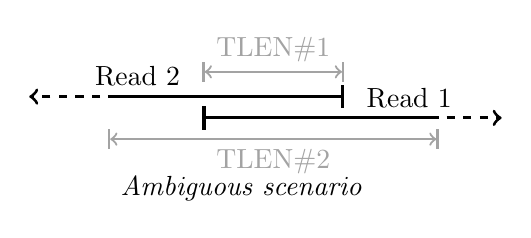
\begin{tikzpicture}[
    thick, xscale=1,yscale=0.9,
    read/.style={line width=0.4mm},
]
\draw[|-, read]         (2.2,0)   -- (5.2,0)    node[very near end, above] {Read 1};
\draw[->, read, dashed] (5.3,0)   -- (6,0);
\draw[-|, read]         (1,.3)    -- (4,.3)     node[very near start , above] {Read 2};
\draw[->, read, dashed] (0.9,.3)  -- (0,.3);
\draw[|<->|,gray!120]   (1,-0.3)  -- (5.2,-0.3) node[midway, below] {TLEN\#2};
\draw[|<->|,gray!120]   (2.2,0.65)-- (4,0.65)    node[midway, above] {TLEN\#1};
\node at (2.7,-1) {\textit{Ambiguous scenario}};
\end{tikzpicture}
\end{center}
}

\item {\sf SEQ}: segment SEQuence. This field can be a `*' when the
  sequence is not stored. If not a `*', the length of the sequence must
  equal the sum of lengths of {\tt M/I/S/=/X} operations in {\sf CIGAR}.
  An `=' denotes the base is identical to the reference base. No
  assumptions can be made on the letter cases.
\item {\sf QUAL}: ASCII of base QUALity plus 33 (same as the quality
  string in the Sanger FASTQ format). A base quality is the phred-scaled
  base error probability which equals $-10\log_{10}\Pr\{\mbox{base is
    wrong}\}$. This field can be a `*' when quality is not stored. If
  not a `*', {\sf SEQ} must not be a `*' and the length of the quality string
  ought to equal the length of {\sf SEQ}.
\end{enumerate}

\subsection{The alignment section: optional fields}\label{sec:alnaux}
All optional fields follow the {\tt TAG:TYPE:VALUE} format
where {\tt TAG} is a two-character string that matches {\tt /[A-Za-z][A-Za-z0-9]/}.
Each {\tt TAG} can only appear once in one alignment line. A {\tt TAG}
containing lowercase letters are reserved for end users.
In an optional field, {\tt TYPE} is a single case-sensitive letter which
defines the format of {\tt VALUE}:
\begin{center}\small
\begin{tabular}{cll}
\hline
{\bf Type} & {\bf Regexp matching {\tt VALUE}} & {\bf Description} \\
\hline
A & {\tt [!-\char126]} & Printable character \\
i & {\tt [-+]?[0-9]+} & Signed integer\footnotemark\\
f & {\tt [-+]?[0-9]*\char92.?[0-9]+([eE][-+]?[0-9]+)?} & Single-precision floating number \\
Z & {\tt [\,\,\,!-\char126]*} & Printable string, including space\\
H & {\tt ([0-9A-F][0-9A-F])*} & Byte array in the Hex format\footnotemark\\
B & {\tt [cCsSiIf](,[-+]?[0-9]*\char92.?[0-9]+([eE][-+]?[0-9]+)?)*} & Integer or numeric array\\
\hline
\end{tabular}
\addtocounter{footnote}{-1}
\footnotetext{The number of digits in an integer optional field is not
explicitly limited in SAM.  However, BAM can represent values in the
range~$[-2^{31},2^{32})$, so in practice this is the realistic range
of values for SAM's `{\tt i}' as well.}
\stepcounter{footnote}
\footnotetext{For example, the six-character Hex string `{\tt 1AE301}' represents the byte array $[{\tt 0x1a},{\tt 0xe3},{\tt 0x1}]$.}
\end{center}
For an integer or numeric array (type `{\tt B}'), the first letter indicates the type of numbers
in the following comma separated array. The letter can be one of `{\tt cCsSiIf}', corresponding to
{\tt int8\_t} (signed 8-bit integer), {\tt uint8\_t} (unsigned 8-bit integer), {\tt int16\_t}, {\tt uint16\_t}, {\tt int32\_t}, {\tt uint32\_t}
and {\tt float}, respectively.\footnotemark\@ During import/export, the element type
may be changed if the new type is also compatible with the array.
\footnotetext{Explicit typing eases format parsing and helps to reduce the file size when SAM is converted to BAM.}

Predefined tags are described in the separate {\sl Sequence Alignment/Map
Optional Fields Specification}.\footnote{See
\href{http://samtools.github.io/hts-specs/SAMtags.pdf}{\tt SAMtags.pdf}
at \url{https://github.com/samtools/hts-specs}.}
See that document for details of existing standard tag fields and conventions
around creating new tags that may be of general interest.
Tags starting with `{\tt X}', `{\tt Y}' or `{\tt Z}' and tags containing
lowercase letters in either position are reserved for local use and will
not be formally defined in any future version of these specifications.

\pagebreak

\section{Recommended Practice for the SAM Format}
\label{sec:recommended-practice}
This section describes the best practice for representing data in the
SAM format. They are not required in general, but may be required by a
specific software package for it to function properly.

\begin{enumerate}
\item The header section
  \begin{enumerate}[label=\arabic*]
  \item The {\tt @HD} line should be present, with either the {\tt SO} tag
    or the {\tt GO} tag (but not both) specified.
  \item The {\tt @SQ} lines should be present if reads have been mapped.
  \item When a {\tt RG} tag appears anywhere in the alignment section,
    there should be a single corresponding {\tt @RG} line with matching
    {\tt ID} tag in the header.
  \item When a {\tt PG} tag appears anywhere in the alignment section,
    there should be a single corresponding {\tt @PG} line with matching
    {\tt ID} tag in the header.
  \end{enumerate}
\item Adjacent CIGAR operations should be different.
\item No alignments should be assigned mapping quality 255.
\item Unmapped reads
  \begin{enumerate}[label=\arabic*]
  \item For a unmapped paired-end or mate-pair read whose mate is
    mapped, the unmapped read should have {\sf RNAME} and {\sf POS}
    identical to its mate.
  \item If all segments in a template are unmapped, their {\sf RNAME}
    should be set as `*' and {\sf POS} as 0.
  \item If {\sf POS} plus the sum of lengths of {\tt M/=/X/D/N}
    operations in {\sf CIGAR} exceeds the length specified in the {\tt
      LN} field of the {\tt @SQ} header line (if exists) with an SN
    equal to {\sf RNAME}, the alignment should be unmapped, unless the
    reference sequence is circular (see below).
  \item Unmapped reads should be stored in the orientation in which they came
    off the sequencing machine and have their {\sf reverse} flag bit~(0x10)
    correspondingly unset.
  \end{enumerate}
\item Multiple mapping
  \begin{enumerate}[label=\arabic*]
  \item When one segment is present in multiple lines to represent a multiple
	mapping of the segment, only one of these records should have the secondary
	alignment flag bit (0x100) unset. {\sf RNEXT} and {\sf PNEXT} point to the
	primary line of the next read in the template.
  \item {\sf SEQ} and {\sf QUAL} of secondary alignments should be set
    to `*' to reduce the file size.
  \end{enumerate}
%\item There should be no overlap between segments of a read\footnote{Few/no
%  existing aligners follow this practice.}.
\item Optional tags:
  \begin{enumerate}[label=\arabic*]
  \item If the template has more than 2 segments, the {\tt TC} tag
    should be present.
  \item The {\tt NM} tag should be present.
  \end{enumerate}

\item Circular reference sequences

Mappings that cross the coordinate `join' in circular reference sequences (i.e., those whose {\tt @SQ} headers specify {\tt TP:circular}) may be represented as follows:
  \begin{enumerate}[label=\arabic*]
  \item (Preferred)
As usual {\sf POS} should be between 1 and the {\tt @SQ} header's {\tt LN} value, but {\sf POS} plus the sum of the lengths of {\tt M/=/X/D/N} {\sf CIGAR} operations may exceed {\tt LN}.
Coordinates greater than~{\tt LN} are interpreted by subtracting {\tt LN} so that bases at $\texttt{LN}+1, \texttt{LN}+2, \texttt{LN}+3, \ldots$ are considered to be mapped at positions $1,2,3,\ldots$; thus each (1-based) position $p$ is interpreted as $((p-1)\bmod\texttt{LN})+1$.%
\footnote{The impact of this representation on indexing and random access is yet to be explored by implementations.}

  \item
Alternatively, such alignments may be split across several records: one record representing the initial portion of the segment ending at~{\tt LN}, one representing the final portion starting from~1, and any other records representing additional portions in between spanning the entire reference sequence.
One record (chosen arbitrarily) is considered primary and the remainder have their {\sf supplementary} flag bit (0x800) set.
  \end{enumerate}

\item Annotation dummy reads:
  These have {\sf SEQ} set to {\tt *}, {\sf FLAG} bits 0x100 and 0x200
  set (secondary and filtered), and a {\tt CT} tag.
  \begin{enumerate}[label=\arabic*]
%Repeating what is in the tag's footnote:
%  \item If the {\tt CT} tag's \emph{strand} is {\tt -}, FLAG bit 0x10
%  (reverse complemented) should be set, and otherwise not set.
  \item If you wish to store free text in a {\tt CT} tag, use the
  \emph{key} value {\tt Note} (uppercase N) to match GFF3.
  \item Multi-segment annotation (e.g., a gene with introns) should be
  described with multiple lines in SAM (like a multi-segment read).
  Where there is a clear biological direction (e.g., a gene), the first
  segment ({\sf FLAG} bit 0x40) is used for the first section (e.g., the
  $5'$ end of the gene). Thus a GenBank entry location like
  {\tt complement(join(85052..85354, 85441..85621, 86097..86284))}
  would have three lines in SAM with a common {\sf QNAME}: %And three lines in GFF3 too.
    \begin{center}\begin{tabular}{llrcl}
  & \multicolumn{1}{c}{\sf FLAG} & \multicolumn{1}{c}{\sf POS} & \sf CIGAR & \multicolumn{1}{c}{Optional fields} \\
The $5'$ fragment & 883 (0x373) & 86097 & \tt 188M & \tt FI:i:1\quad TC:i:3 \\
Middle fragment   & 819 (0x333) & 85441 & \tt 181M & \tt FI:i:2\quad TC:i:3 \\
The $3'$ fragment & 947 (0x3B3) & 85052 & \tt 303M & \tt FI:i:3\quad TC:i:3
    \end{tabular}\end{center}
  \item If converting GFF3 to SAM, store any \emph{key}, \emph{values}
  from column 9 in the {\tt CT} tag, except for the unique ID which
  is used for the QNAME. GFF3 columns 1 (seqid), 4 (start) and 5 (end)
  are encoded using SAM columns RNAME, POS and CIGAR to hold the length.
  GFF3 columns 3 (type) and 7 (strand) are stored explicitly in the
  {\tt CT} tag. Remaining GFF3 columns 2 (source), 6 (score), and
  8 (phase) are stored in the {\tt CT} tag using \emph{key} values
  {\tt FSource}, {\tt FScore} and {\tt FPhase} (uppercase keys are
  restricted in GFF3, so these names avoid clashes). Split location
  features are described with multiple lines in GFF3, and similarly
  become multi-segment dummy reads in SAM, with the {\sf RNEXT} and
  {\sf PNEXT} columns filled in appropriately. In the absence of a
  convention in SAM/BAM for reads wrapping the origin of a circular
  genome, any GFF3 feature line wrapping the origin must be split into
  two segments in SAM.
  \end{enumerate}
\end{enumerate}

\section{Guide for Describing Assembly Sequences in SAM}

\subsection{Unpadded versus padded representation}

To describe alignments, we can regard the reference sequence with no respect to
other alignments against it.  Such a reference sequence is called an
\emph{unpadded reference}. A position on an unpadded reference, referred to
as an \emph{unpadded position}, is not affected by any alignments. When we use
unpadded references and positions to describe alignments, we say we are using
the \emph{unpadded representation}.

Alternatively, to describe the same alignments, we can modify the reference
sequence to contain pads that make room for sequences inserted relative to the
reference. A pad is effectively a gap and conventionally represented by an
asterisk `*'.  A reference sequence containing pads is called a \emph{padded
reference}. A position which counts the *'s is referred to as a \emph{padded
position}. A padded reference sequence may be affected by the query alignments
and because of gap insertions is typically longer than the unpadded reference.
The padded position of one query alignment may be affected by other query
alignments.

Unpadded and padded are different representations of the same alignments. They
are convertible to each other with no loss of any information. The unpadded
representation is more common due to the convenience of a fixed coordinate system,
while the padded representation has the advantage that alignments can be simply
described by the start and end coordinates without using complex CIGAR strings.
SAM traditionally uses the padded representation for {\it de novo} assembly.
The ACE assembly format uses the padded representation exclusively.

\subsection{Padded SAM}\label{sec:padded-sam}

The SAM format is typically used to describe alignments against an unpadded
reference sequence, but it is also able to describe alignments against a padded
reference. In the latter case, we say we are using a \emph{padded SAM}. A padded
SAM is a valid SAM, but with the difference that the reference and positions in
use are padded. There may be more than one way to describe the padded
representation.
We recommend the following; see also the discussion in Cock {\it et al.}%
\footnote{Peter J. A. Cock, James K. Bonfield, Bastien Chevreux, and Heng Li,
{\bf SAM/BAM format v1.5 extensions for \emph{de novo} assemblies},
{\sl bioRxiv 020024};
\href{http://dx.doi.org/10.1101/020024}{doi:10.1101/020024}.}

In a padded SAM, alignments and coordinates are described with respect to the
padded reference sequence. Unlike traditional padded representations like
the ACE file format where pads/gaps are recorded in reads using *'s, we do
not write *'s in the {\sf SEQ} field of the SAM format.\footnote{Writing
pads/gaps as *'s in the {\sf SEQ} field might have been more convenient, but
this caused concerns for backward compatibility.} Instead, we describe pads
in the query sequences as deletions from the padded reference using the
{\sf CIGAR} `{\tt D}' operation. In a padded SAM, the insertion and padding
CIGAR operations (`{\tt I}' and `{\tt P}') are not used because the padded
reference already considers all the insertions.

The following shows the padded SAM for the example alignment in Section~\ref{sec:example}.
Notably, the length of {\tt ref} is 47 instead of 45. {\sf POS} of the last
three alignments are all shifted by 2. {\sf CIGAR} of alignments bridging the
2bp insertion are also changed.

\begin{framed}\small
\begin{verbatim}
@HD VN:1.6 SO:coordinate
@SQ SN:ref LN:47
ref   516 ref  1  0 14M2D31M   *  0   0 AGCATGTTAGATAAGATAGCTGTGCTAGTAGGCAGTCAGCGCCAT *
r001   99 ref  7 30 14M1D3M    = 39  41 TTAGATAAAGGATACTG *
*     768 ref  8 30 1M         *  0   0 *                 * CT:Z:.;Warning;Note=Ref wrong?
r002    0 ref  9 30 3S6M1D5M   *  0   0 AAAAGATAAGGATA    * PT:Z:1;4;+;homopolymer
r003    0 ref  9 30 5H6M       *  0   0 AGCTAA            * NM:i:1
r004    0 ref 18 30 6M14N5M    *  0   0 ATAGCTTCAGC       *
r003 2064 ref 31 30 6H5M       *  0   0 TAGGC             * NM:i:0
r001  147 ref 39 30 9M         =  7 -41 CAGCGGCAT         * NM:i:1
\end{verbatim}
\end{framed}

Here we also exemplify the recommended practice for storing the reference
sequence and the reference annotations in SAM when necessary. For a reference
sequence in SAM, {\sf QNAME} should be identical to {\sf RNAME}, {\sf POS} set
to 1 and {\sf FLAG} to 516 (filtered and unmapped); for an annotation, {\sf
FLAG} should be set to 768 (filtered and secondary) with no restriction to {\sf
QNAME}.
Dummy reads for annotation would typically have a {\tt CT} tag to hold the annotation information; see the discussion of dummy reads in Section~\ref{sec:recommended-practice}.
See also the separate {\sl Optional Fields Specification} for full details of the {\tt CT} and {\tt PT} annotation tags.%
\footnote{See \emph{Annotation and Padding} in \href{http://samtools.github.io/hts-specs/SAMtags.pdf}{\tt SAMtags.pdf}.}

\pagebreak

\section{The BAM Format Specification}

\subsection{The BGZF compression format}

BGZF is block compression implemented on top of the standard gzip file
format.\footnote{L.~Peter Deutsch, {\bf GZIP file format specification
version~4.3}, \href{http://tools.ietf.org/html/rfc1952}{\sl RFC 1952}.}
The goal of BGZF is to provide good compression while allowing
efficient random access to the BAM file for indexed queries. The BGZF
format is `gunzip compatible', in the sense that a compliant gunzip
utility can decompress a BGZF compressed file.\footnote{It is worth noting that there is a known bug in the Java {\sf
  GZIPInputStream} class that concatenated gzip archives cannot be
successfully decompressed by this class. BGZF files can be created and
manipulated using the built-in Java {\sf util.zip} package, but naive
use of {\sf GZIPInputStream} on a BGZF file will not work due to this
bug.}

A BGZF file is a series of concatenated BGZF blocks, each no larger
than~64Kb before or after compression. Each BGZF block
is itself a spec-compliant gzip archive which contains an ``extra field''
in the format described in RFC1952. The gzip file format allows the
inclusion of application-specific extra fields and these are ignored by
compliant decompression implementation. The gzip specification also
allows gzip files to be concatenated. The result of decompressing
concatenated gzip files is the concatenation of the uncompressed data.

Each BGZF block contains a standard gzip file header with the following
standard-compliant extensions:

\begin{enumerate}
\item The {\sf F.EXTRA} bit in the header is set to indicate that extra
  fields are present.
\item The extra field used by BGZF uses the two subfield ID values 66 and 67 (ascii `BC').
\item The length of the BGZF extra field payload (field {\sf LEN} in the
  gzip specification) is 2 (two bytes of payload).
\item The payload of the BGZF extra field is a 16-bit unsigned integer
  in little endian format. This integer gives the size of the containing
  BGZF block minus one.
\end{enumerate}

On disk, a complete BGZF file is a series of blocks as shown in the following
table.  (All integers are little endian as is required by RFC1952.)
\begin{table}[ht]
\centering
{\small
\begin{tabular}{|l|l|l|l|l|r|}
  \cline{1-6}
  \multicolumn{3}{|c|}{\bf Field} & \multicolumn{1}{c|}{\bf Description} & \multicolumn{1}{c|}{\bf Type} & \multicolumn{1}{c|}{\bf Value} \\\cline{1-6}
  \multicolumn{6}{|c|}{\textcolor{gray}{\it List of compression blocks (until the end of the file)}} \\\cline{2-6}
  & \multicolumn{2}{l|}{\sf ID1} & gzip IDentifier1 & {\tt uint8\_t} & 31 \\\cline{2-6}
  & \multicolumn{2}{l|}{\sf ID2} & gzip IDentifier2 & {\tt uint8\_t} & 139 \\\cline{2-6}
  & \multicolumn{2}{l|}{\sf CM} & gzip Compression Method & {\tt uint8\_t} & 8 \\\cline{2-6}
  & \multicolumn{2}{l|}{\sf FLG} & gzip FLaGs & {\tt uint8\_t} & 4 \\\cline{2-6}
  & \multicolumn{2}{l|}{\sf MTIME} & gzip Modification TIME & {\tt uint32\_t} & \\\cline{2-6}
  & \multicolumn{2}{l|}{\sf XFL} & gzip eXtra FLags & {\tt uint8\_t} & \\\cline{2-6}
  & \multicolumn{2}{l|}{\sf OS} & gzip Operating System & {\tt uint8\_t} & \\\cline{2-6}
  & \multicolumn{2}{l|}{\sf XLEN} & gzip eXtra LENgth & {\tt uint16\_t} & \\\cline{2-6}
  & \multicolumn{5}{c|}{\textcolor{gray}{\it Extra subfield(s) (total size=XLEN)}} \\\cline{3-6}
  & & \multicolumn{4}{c|}{\textcolor{gray}{\it Additional RFC1952 extra subfields if present}} \\\cline{3-6}
  & & {\sf SI1} & Subfield Identifier1 & {\tt uint8\_t} & 66 \\\cline{3-6}
  & & {\sf SI2} & Subfield Identifier2 & {\tt uint8\_t} & 67 \\\cline{3-6}
  & & {\sf SLEN} & Subfield LENgth & {\tt uint16\_t} & 2 \\\cline{3-6}
  & & {\sf BSIZE} & total Block SIZE minus 1 & {\tt uint16\_t} & \\\cline{3-6}
  & & \multicolumn{4}{c|}{\textcolor{gray}{\it Additional RFC1952 extra subfields if present}} \\\cline{2-6}
  & \multicolumn{2}{l|}{\sf CDATA} & Compressed DATA by {\sf zlib::deflate()} & {\tt uint8\_t[{\sf BSIZE-XLEN-19}]} & \\\cline{2-6}
  & \multicolumn{2}{l|}{\sf CRC32} & CRC-32 & {\tt uint32\_t} & \\\cline{2-6}
  & \multicolumn{2}{l|}{\sf ISIZE} & Input SIZE (length of uncompressed data) & {\tt uint32\_t} & \\
  \cline{1-6}
\end{tabular}}
\end{table}

The random access method to be described next limits the uncompressed
contents of each BGZF block to a maximum of $2^{16}$~bytes of data.
Thus while {\sf ISIZE} is stored as a {\tt uint32\_t} as per the gzip format,
in BGZF it is limited to the range~$[0,65536]$.
{\sf BSIZE} can represent BGZF block sizes in the range~$[1,65536]$, though
typically {\sf BSIZE} will be rather less than~{\sf ISIZE} due to compression.

\subsubsection{Random access}

BGZF files support random access through the BAM file index. To achieve
this, the BAM file index uses \emph{virtual file offsets} into the BGZF
file. Each virtual file offset is an unsigned 64-bit integer, defined as: {\tt
  coffset\char60\char60 16\char124uoffset}, where {\tt coffset} is an
unsigned byte offset into the BGZF file to the beginning of a BGZF
block, and {\tt uoffset} is an unsigned byte offset into the
uncompressed data stream represented by that BGZF block. Virtual file
offsets can be compared, but subtraction between virtual file offsets
and addition between a virtual offset and an integer are both
disallowed.

\subsubsection{End-of-file marker}

An end-of-file (EOF) trailer or marker block should be written at the end
of BGZF files, so that unintended file truncation can be easily detected.
The EOF marker block is a particular empty\footnotemark\ BGZF block
encoded with the default {\sf zlib} compression level settings,
and consists of the following 28~hexadecimal bytes:
\begin{center}
\texttt{1f 8b 08 04 00 00 00 00 00 ff 06 00 42 43 02 00 1b 00 03 00 00 00 00 00 00 00 00 00}
\end{center}

\footnotetext{Empty in the sense of having been formed by compressing
a data block of length zero.}

\noindent
The presence of this EOF marker at the end of a BGZF file indicates that the
immediately following physical EOF is the end of the file as intended by the
program that wrote it.
Empty BGZF blocks are not otherwise special; in particular, the presence of
an EOF marker block does not by itself signal end of file.\footnotemark

\footnotetext{An implementation that supports reopening a BAM file in append
mode could produce a file by writing headers and alignment records to it,
closing it (adding an EOF marker); then reopening it for append, writing
more alignment records, and closing it (adding an EOF marker).
The resulting BAM file would contain an embedded insignificant EOF~marker
block that should be effectively ignored when it is read.}

The absence of this final EOF marker should trigger a warning or error
soon after opening a BGZF file where random access is available.\footnotemark\
When reading a BGZF file in sequential streaming fashion, ideally this
EOF check should be performed when the end of the stream is reached.
Checking that the final BGZF block in the file decompresses to empty
or checking that the last 28 bytes of the file are exactly the bytes
above are both sufficient tests; each is likely more convenient in
different circumstances.

\footnotetext{It is useful to produce a diagnostic at the beginning of
reading a file, so that interactive users can abort lengthy analysis of
potentially-corrupted files.  Of course, this is only possible if the
stream in question supports random access.}

\pagebreak

\subsection{The BAM format}
BAM is compressed in the BGZF format. All multi-byte numbers in BAM are
little-endian, regardless of the machine endianness. The format is
formally described in the following table where values in brackets are
the default when the corresponding information is not available; an
underlined word in uppercase denotes a field in the SAM format.

\begin{table}[ht]
\centering
{\small
\begin{tabular}{|l|l|l|p{8.15cm}|l|r|}
  \cline{1-6}
  \multicolumn{3}{|c|}{\bf Field} & \multicolumn{1}{c|}{\bf Description} & \multicolumn{1}{c|}{\bf Type} & \multicolumn{1}{c|}{\bf Value} \\\cline{1-6}
  \multicolumn{3}{|l|}{\sf magic} & BAM magic string & {\tt char[4]} & {\tt BAM\char92 1}\\\cline{1-6}
  \multicolumn{3}{|l|}{\sf l\_text} & Length of the header text, including any {\tt NUL} padding & {\tt uint32\_t} & $< 2^{31}$ \\\cline{1-6}
  \multicolumn{3}{|l|}{\sf text} & Plain header text in SAM; not necessarily {\tt NUL}-terminated & {\tt char[{\sf l\_text}]} & \\\cline{1-6}
  % Pedantically this should be <= but we restrict |refs| by one so n_ref fits in a signed 32-bit int.
  \multicolumn{3}{|l|}{\sf n\_ref} & \# reference sequences & {\tt uint32\_t} & $< 2^{31}$ \\\cline{1-6}
  \multicolumn{6}{|c|}{\textcolor{gray}{\it List of reference information (n=n\_ref)}} \\\cline{2-6}
  & \multicolumn{2}{l|}{\sf l\_name} & Length of the reference name plus 1 (including {\tt NUL}) & {\tt uint32\_t} & \memlimited \\\cline{2-6}
  & \multicolumn{2}{l|}{\sf name} & Reference sequence name; {\tt NUL}-terminated & {\tt char[{\sf l\_name}]} & \\\cline{2-6}
  & \multicolumn{2}{l|}{\sf l\_ref} & Length of the reference sequence & {\tt uint32\_t} & $< 2^{31}$ \\\cline{1-6}
  \multicolumn{6}{|c|}{\textcolor{gray}{\it List of alignments (until the end of the file)}} \\\cline{2-6}
  & \multicolumn{2}{l|}{\sf block\_size} & Total length of the alignment record, excluding this field & {\tt uint32\_t} & \memlimited \\\cline{2-6}
  & \multicolumn{2}{l|}{\sf refID} & Reference sequence ID, $-1\leq{\sf refID}<{\sf n\_ref}$; -1 for a read without a mapping position & {\tt int32\_t} & [-1] \\\cline{2-6}
  & \multicolumn{2}{l|}{\sf pos} & 0-based leftmost coordinate ($=\underline{\sf POS}-1$)& {\tt int32\_t} & [-1]\\\cline{2-6}
  & \multicolumn{2}{l|}{\sf l\_read\_name} & Length of {\sf read\_name} below ($={\sf length}(\underline{\sf QNAME})+1$) & {\tt uint8\_t} & \\\cline{2-6}
  & \multicolumn{2}{l|}{\sf mapq} & Mapping quality (=\underline{\sf MAPQ}) & {\tt uint8\_t} & \\\cline{2-6}
  & \multicolumn{2}{l|}{\sf bin} & BAI index bin, see Section~\ref{sec:bin-field}  & {\tt uint16\_t} & \\\cline{2-6}
  & \multicolumn{2}{l|}{\sf n\_cigar\_op} & Number of operations in \underline{\sf CIGAR}, see Section~\ref{sec:ncigar} & {\tt uint16\_t} & \\\cline{2-6}
  & \multicolumn{2}{l|}{\sf flag} & Bitwise flags (= \underline{\sf FLAG})\footnotemark\ & {\tt uint16\_t} & \\\cline{2-6}
  & \multicolumn{2}{l|}{\sf l\_seq} & Length of \underline{\sf SEQ} & {\tt uint32\_t} & \memlimited \\\cline{2-6}
  & \multicolumn{2}{l|}{\sf next\_refID} & Ref-ID of the next segment ($-1\le{\sf next\_refID}<{\sf n\_ref}$) & {\tt int32\_t} & [-1] \\\cline{2-6}
  & \multicolumn{2}{l|}{\sf next\_pos} & 0-based leftmost pos of the next segment ($=\underline{\sf PNEXT}-1$) & {\tt int32\_t} & [-1] \\\cline{2-6}
  & \multicolumn{2}{l|}{\sf tlen} & Template length ($=\underline{\sf TLEN}$) & {\tt int32\_t} & [0] \\\cline{2-6}
  & \multicolumn{2}{l|}{\sf read\_name} & Read name, {\tt NUL}-terminated (\underline{\sf QNAME} with trailing `{\tt\verb"\0"}')\footnotemark & {\tt char[{\sf l\_read\_name}]} & \\\cline{2-6}
  & \multicolumn{2}{l|}{\sf cigar} & CIGAR: {\tt {\sf op\_len}\char60\char60 4\char124{\sf op}}. `{\tt MIDNSHP\char61X}'$\to$`012345678' & {\tt uint32\_t[{\sf n\_cigar\_op}]} & \\\cline{2-6}
  & \multicolumn{2}{l|}{\sf seq} & 4-bit encoded read: `{\tt =ACMGRSVTWYHKDBN}'$\to[0,15]$. See Section~\ref{sec:seq} & {\tt uint8\_t[({\sf l\_seq}+1)/2]} & \\\cline{2-6}
  & \multicolumn{2}{l|}{\sf qual} & Phred-scaled base qualities. See Section~\ref{sec:seq} & {\tt char[{\sf l\_seq}]} & \\\cline{2-6}
  & \multicolumn{5}{c|}{\textcolor{gray}{\it List of auxiliary data (until the end of the alignment block)}} \\\cline{3-6}
  & & {\sf tag} & Two-character tag & {\tt char[2]} & \\\cline{3-6}
  & & {\sf val\_type} & Value type: {\tt AcCsSiIfZHB}, see Section~\ref{sec:aux-type-codes} & {\tt char} & \\\cline{3-6}
  & & {\sf value} & Tag value & (by {\sf val\_type}) &\\
  \cline{1-6}
\end{tabular}}
\end{table}
\addtocounter{footnote}{-1}
\footnotetext{As noted in Section~\ref{sec:alnrecord}, reserved {\sf FLAG} bits
should be written as zero and ignored on reading by current software.}
\stepcounter{footnote}
\footnotetext{For backward compatibility, an absent {\sf QNAME} (represented as `{\tt *}' in SAM) is stored as a C string {\tt "*\char92 0"}.}

\noindent
Most length and count fields described as {\tt uint32\_t} have additional constraints on their range:
$\mbox{\sf l\_text} < 2^{31}$ due to implementation limits;
$\mbox{\sf n\_ref} < 2^{31}$ because {\sf refID} and {\sf next\_refID} are signed;
$\mbox{\sf l\_ref} < 2^{31}$ because {\sf tlen} is signed;
those marked ``\textit{limited}'' are limited by available memory and the practical size of the data represented well before they are limited by, e.g., Java's signed 32-bit integer maximum array size.

\subsubsection{BIN field calculation}\label{sec:bin-field}
{\sf BIN} is calculated using the {\sf reg2bin()} function in
Section~\ref{sec:code}.
For mapped reads this uses {\sf POS-1} (i.e.,~0-based left position) and the
alignment end point using the alignment length from the {\sf CIGAR} string.
For unmapped reads (e.g.,~paired end reads where only one part is mapped, see
Section~\ref{sec:recommended-practice}) the alignment is treated as
being length one.
Note unmapped reads with {\sf POS} $0$ (which becomes $-1$ in BAM) therefore
use {\sf reg2bin(-1, 0)} which is $4680$.

\subsubsection{N\_CIGAR\_OP field}\label{sec:ncigar}
With 16 bits, {\sf n\_cigar\_op} can keep at most 65535 CIGAR
operations in BAM files. For an alignment with more CIGAR operations, BAM
stores the real {\sf CIGAR}, encoded the same way as the {\sf cigar} field in
BAM, in the {\tt CG} optional tag of type `{\tt B,I}', and sets {\sf CIGAR} to
`\textit{k}{\tt S}\textit{m}{\tt N}' as a placeholder, where `\textit{k}' equals {\sf l\_seq}, `\textit{m}'
is the reference sequence length in the alignment, and `{\tt S}' and `{\tt N}'
are the soft-clipping and reference-clip CIGAR operators, respectively---i.e.,
in the binary form, {\sf n\_cigar\_op}=2 and {\sf cigar}={\tt [\textit{k}\char60\char60
4\char124{4},\textit{m}\char60\char60 4\char124{3}]}. If tag {\tt CG} is present and
the first CIGAR operation clips the entire read, a BAM parsing library is
expected to update {\sf n\_cigar\_op} and {\sf cigar} with the real CIGAR
stored in the {\tt CG} tag and remove the now-redundant {\tt CG} tag.

\subsubsection{SEQ and QUAL encoding}\label{sec:seq}
Sequence is encoded in 4-bit values, with adjacent bases packed into the same byte starting with the highest 4 bits first.
When {\sf l\_seq} is odd the bottom 4 bits of the last byte are undefined, but we recommend writing these as zero.
The case-insensitive base codes `{\tt =ACMGRSVTWYHKDBN}' are mapped to $[0,15]$ respectively with all other characters mapping to `{\tt N}' (value 15).

Omitted sequence, represented in SAM as `{\tt *}', is represented by {\sf l\_seq} being 0 and {\sf seq} and {\sf qual} zero-length.

Base qualities are stored as bytes in the range $[0,93]$, without any +33 conversion to printable ASCII.
When base qualities are omitted but the sequence is not, {\sf qual} is filled with {\tt 0xFF} bytes (to length {\sf l\_seq}).

\subsubsection{Auxiliary data encoding}\label{sec:aux-type-codes}
Optional alignment fields are stored immediately after each other immediately
following the {\sf qual} field, and are included in {\sf block\_size}.
Each field is represented as a two-character tag followed by a single type
character and then its value, whose length is determined by the field's type.

\newcommand*{\tagfield}[2]{\firstbytebox{2}{\em tag}\bytebox{1}{\tt #1}#2}

Single character `{\tt A}' fields have a total length of 4~bytes,
with the value represented as a single byte:
\begin{center}\small\byteboxsetup
\tagfield{A}{\bytebox{1}{char}}
\end{center}

While all single (i.e., non-array) integer types are stored in SAM as `{\tt i}',
in BAM any of `{\tt cCsSiI}' may be used together with the correspondingly-sized
binary integer value, chosen according to the field value's magnitude.%
\footnote{The signedness and size used for each integer value is an
implementation choice, but is typically the smallest that suffices.}
Similarly floating point `{\tt f}' fields are represented as IEEE 754-2008
binary32 values.
Thus BAM numeric fields have a total length of~4, 5, or~7~bytes:
\begin{center}\small\byteboxsetup\begin{tabular}{l@{\hspace{1in}}l}
\tagfield{c}{\bytebox{1}{i8}} \quad (i.e., {\tt int8\_t})
    & \tagfield{i}{\bytebox{4}{int32\_t}} \\
\tagfield{C}{\bytebox{1}{u8}} \quad (i.e., {\tt uint8\_t})
    & \tagfield{I}{\bytebox{4}{uint32\_t}} \\
\tagfield{s}{\bytebox{2}{int16\_t}}
    & \tagfield{f}{\bytebox{4}{float}} \\
\tagfield{S}{\bytebox{2}{uint16\_t}}
    &
\end{tabular}\end{center}

\newcommand*{\byteboxvector}[2]{\bytebox{#1}{#2}\bytebox{#1}{#2}\makebox[1.5\bytewidth][c]{$\cdots$}\firstbytebox{#1}{#2}}

String fields and hex-formatted byte arrays are represented as
{\tt NUL}-terminated text strings:%
\footnote{The BAM representation of `{\tt H}' field values as textual
hexadecimal digits rather than binary data is for historical reasons.
Modern applications may prefer to use `{\tt B,C}' array fields rather
than `{\tt H}' fields.}
\begin{center}\small\byteboxsetup\begin{tabular}{l}
\tagfield{Z}{\byteboxvector{1}{char}\bytebox{1}{\tt NUL}} \\
\tagfield{H}{\byteboxvector{2}{hex hex}\bytebox{1}{\tt NUL}}
\end{tabular}\end{center}

\newcommand*{\arraytagfield}[3]{\tagfield{B}{\bytebox{1}{\tt #1}\bytebox{4}{\em count}\byteboxvector{#2}{#3}}}

\begin{samepage}
The representation of a `{\tt B}' array field starts with a sub-type character
similar to the numeric field types above and a \emph{count} ({\tt uint32\_t}, but
limited by memory and {\sf block\_size}) giving the number of elements in the array.
The array elements follow, encoded as binary integers or IEEE floats sized
according to the sub-type:
\begin{center}\small\byteboxsetup\begin{tabular}{l}
\arraytagfield{c}{1}{i8} \quad (i.e., {\tt int8\_t} elements) \\
\arraytagfield{C}{1}{u8} \quad (i.e., {\tt uint8\_t} elements) \\
\arraytagfield{s}{2}{int16\_t} \\
\arraytagfield{S}{2}{uint16\_t} \\
\arraytagfield{i}{4}{int32\_t} \\
\arraytagfield{I}{4}{uint32\_t} \\
\arraytagfield{f}{4}{float}
\end{tabular}\end{center}
\end{samepage}

\pagebreak

\section{Indexing BAM}
Indexing aims to achieve fast retrieval of alignments overlapping a
specified region without going through the whole alignments. BAM must be
sorted by the reference ID and then the leftmost coordinate before
indexing.

This section describes the binning scheme underlying coordinate-sorted
BAM indices and its implementation in the long-established BAI format.
The CSI format documented elsewhere uses a similar binning scheme and
can also be used to index BAM.\footnotemark

\footnotetext{See \href{http://samtools.github.io/hts-specs/CSIv1.pdf}
{\tt CSIv1.pdf} at \url{https://github.com/samtools/hts-specs}.
This is a separate specification because CSI is also used to index other
coordinate-sorted file formats in addition to BAM.}

\subsection{Algorithm}
\subsubsection{Basic binning index}
The UCSC binning scheme was suggested by Richard Durbin and Lincoln Stein
and is explained in Kent {\it et al.}\footnotemark\ In this scheme, each bin
represents a contiguous genomic region which is either fully contained
in or non-overlapping with another bin; each alignment is associated
with a bin which represents the smallest region containing the entire
alignment. The binning scheme is essentially a representation of
R-tree. A distinct bin uniquely corresponds to a distinct internal node
in a R-tree. Bin A is a child of Bin B if the region represented by A is
contained in B.

\footnotetext{W.~James Kent {\it et al.},
{\bf The Human Genome Browser at UCSC}, {\sl Genome Res.}~2002~12: 996--1006;
\href{http://dx.doi.org/doi:10.1101/gr.229102}{doi:10.1101/\linebreak[1]gr.229102};
{\sc pmid:}12045153.  See in particular {\sl The Database}, p1003.}

To find the alignments that overlap a specified region, we need to get
the bins that overlap the region, and then test each alignment in the
bins to check overlap. To quickly find alignments associated with a
specified bin, we can keep in the index the start file offsets of chunks
of alignments which all have the bin. As alignments are sorted by the
leftmost coordinates, alignments having the same bin tend to be
clustered together on the disk and therefore usually a bin is only
associated with a few chunks. Traversing all the alignments having the
same bin usually needs a few seek calls. Given the set of bins that
overlap the specified region, we can visit alignments in the order of
their leftmost coordinates and stop seeking the rest when an alignment
falls outside the required region. This strategy saves half of the seek
calls in average.

In the BAI format, each bin may span $2^{29}$, $2^{26}$, $2^{23}$, $2^{20}$,
$2^{17}$ or $2^{14}$ bp. Bin 0 spans a 512Mbp region, bins 1--8 span 64Mbp,
9--72 8Mbp, 73--584 1Mbp, 585--4680 128Kbp, and bins 4681--37448 span 16Kbp
regions.  This implies that this index format does not support reference
chromosome sequences longer than $2^{29}-1$.

The CSI format generalises the sizes of the bins, and supports reference
sequences of the same length as are supported by SAM and BAM.

\subsubsection{Reducing small chunks}
Around the boundary of two adjacent bins, we may see many small chunks
with some having a shorter bin while the rest having a larger bin. To
reduce the number of seek calls, we may join two chunks having the same
bin if they are close to each other. After this process, a joined chunk
will contain alignments with different bins. We need to keep in the
index the file offset of the end of each chunk to identify its
boundaries.

\subsubsection{Combining with linear index}
For an alignment starting beyond 64Mbp, we always need to seek to some
chunks in bin 0, which can be avoided by using a linear index. In the
linear index, for each tiling 16384bp window on the reference, we record
the smallest file offset of the alignments that overlap with the
window. Given a region [rbeg,\,rend), we only need to visit a chunk whose
end file offset is larger than the file offset of the 16kbp window
containing rbeg.

With both binning and linear indices, we can retrieve alignments in most
of regions with just one seek call.

\subsubsection{A conceptual example}
Suppose we have a genome shorter than 144kbp. We can design a binning
scheme which consists of three types of bins: bin 0 spans 0-144kbp, bin
1, 2 and 3 span 48kbp and bins from 4 to 12 span 16kbp each:

\begin{table}[ht]
  \centering
  {\small\begin{tabular}{|c|c|c|c|c|c|c|c|c|}
    \cline{1-9}
    \multicolumn{9}{|c|}{0 (0--144kbp)}\\\cline{1-9}
    \multicolumn{3}{|c|}{1 (0--48kbp)} & \multicolumn{3}{c|}{2 (48--96kbp)} & \multicolumn{3}{c|}{3 (96--144kbp)} \\\cline{1-9}
    4 (0--16k) & 5 (16--32k) & 6 (32--48k) & 7 (48--64k) & 8 (64--80k) & 9 (80--96k) & 10 & 11 & 12 \\
    \cline{1-9}
  \end{tabular}}
\end{table}

An alignment starting at 65kbp and ending at 67kbp would have a bin
number 8, which is the smallest bin containing the alignment. Similarly,
an alignment starting at 51kbp and ending at 70kbp would go to bin 2,
while an alignment between [40k,\,49k] to bin 0. Suppose we want to find
all the alignments overlapping region [65k,\,71k). We first calculate that
bin 0, 2 and 8 overlap with this region and then traverse the alignments
in these bins to find the required alignments. With a binning index
alone, we need to visit the alignment at [40k,\,49k] as it belongs to bin
0. But with a linear index, we know that such an alignment stops before
64kbp and cannot overlap the specified region. A seek call can thus be
saved.

\subsection{The BAI index format for BAM files}
\begin{table}[ht]
\centering\small
\begin{tabular}{|l|l|l|l|l|l|r|}
  \cline{1-7}
  \multicolumn{4}{|c|}{\bf Field} & \multicolumn{1}{c|}{\bf Description} & \multicolumn{1}{c|}{\bf Type} & \multicolumn{1}{c|}{\bf Value} \\\cline{1-7}
  \multicolumn{4}{|l|}{\sf magic} & Magic string & {\tt char[4]} & {\tt BAI\char92 1}\\\cline{1-7}
  \multicolumn{4}{|l|}{\sf n\_ref} & \# reference sequences & {\tt uint32\_t} & $< 2^{31}$ \\\cline{1-7}
  \multicolumn{7}{|c|}{\textcolor{gray}{\it List of indices (n=n\_ref)}} \\\cline{2-7}
  & \multicolumn{3}{l|}{\sf n\_bin} & \# distinct bins (for the binning index) & {\tt uint32\_t} & $\le 37451$ \\\cline{2-7}
  & \multicolumn{6}{c|}{\textcolor{gray}{\it List of distinct bins (n=n\_bin)}} \\\cline{3-7}
  & & \multicolumn{2}{l|}{\sf bin} & Distinct bin & {\tt uint32\_t} & $\le 37450$ \\\cline{3-7}
  & & \multicolumn{2}{l|}{\sf n\_chunk} & \# chunks & {\tt uint32\_t} & \memlimited\footnotemark \\\cline{3-7}
  & & \multicolumn{5}{c|}{\textcolor{gray}{\it List of chunks (n=n\_chunk)}} \\\cline{4-7}
  & & & {\sf chunk\_beg} & (Virtual) file offset of the start of the chunk & {\tt uint64\_t} & \\\cline{4-7}
  & & & {\sf chunk\_end} & (Virtual) file offset of the end of the chunk & {\tt uint64\_t} & \\\cline{2-7}
  & \multicolumn{3}{l|}{\sf n\_intv} & \# 16kbp intervals (for the linear index) & {\tt uint32\_t} & $\le 2^{17}$ \\\cline{2-7}
  & \multicolumn{6}{c|}{\textcolor{gray}{\it List of intervals (n=n\_intv)}} \\\cline{3-7}
  & & \multicolumn{2}{l|}{\sf ioffset} & (Virtual) file offset of the first alignment in the interval & {\tt uint64\_t} & \\\cline{1-7}
  \multicolumn{4}{|l|}{{\sf n\_no\_coor} (optional)} & Number of unplaced unmapped reads ({\sf RNAME} *) & {\tt uint64\_t} & \\\cline{1-7}
\end{tabular}
\end{table}

\footnotetext{The number of chunks in a single bin is effectively limited by available memory and in any case is typically a maximum of some thousands.}

The index file may optionally contain additional metadata providing a summary
of the number of mapped and unmapped read-segments per reference sequence,
and of any unplaced unmapped read-segments.\footnote{By \emph{placed unmapped
read} we mean a read that is unmapped according to its {\sf FLAG} but whose
{\sf RNAME} and~{\sf POS} fields are filled in, thus ``placing'' it on a
reference sequence (see Section~\ref{sec:recommended-practice}).
In contrast, \emph{unplaced} unmapped reads have~`*' and~0 for {\sf RNAME}
and~{\sf POS}.}
This is stored in an optional extra metadata pseudo-bin for each reference
sequence, and in the optional trailing {\sf n\_no\_coor} field at the end of
the file.

The pseudo-bins appear in the references' lists of distinct bins as bin
number~37450 (which is beyond the normal range) and are laid out so as to be
compatible with real bins and their chunks:

\begin{table}[ht]
\centering\small
\begin{tabular}{|l|l|l|r|}
  \hline
  {\sf bin} & Magic bin number & {\tt uint32\_t} & 37450 \\\hline
  {\sf n\_chunk} & \# chunks & {\tt uint32\_t} & 2 \\\hline
  {\sf unmapped\_beg} & (Virtual) file offset of the start of placed unmapped reads & {\tt uint64\_t} & \\\hline
  {\sf unmapped\_end} & (Virtual) file offset of the end of placed unmapped reads & {\tt uint64\_t} & \\\hline
  {\sf n\_mapped} & Number of mapped read-segments for this reference & {\tt uint64\_t} & \\\hline
  {\sf n\_unmapped} & Number of unmapped read-segments for this reference & {\tt uint64\_t} & \\\hline
\end{tabular}
\end{table}

\subsection{C source code for computing bin number and overlapping bins}\label{sec:code}
The following functions compute bin numbers and overlaps for a BAI-style
binning scheme with $6$~levels and a minimum bin size of $2^{14}$~bp.
See the CSI specification for generalisations of these functions designed for
binning schemes with arbitrary depth and sizes.

{\small
\begin{verbatim}
/* calculate bin given an alignment covering [beg,end) (zero-based, half-closed-half-open) */
int reg2bin(int beg, int end)
{
    --end;
    if (beg>>14 == end>>14) return ((1<<15)-1)/7 + (beg>>14);
    if (beg>>17 == end>>17) return ((1<<12)-1)/7 + (beg>>17);
    if (beg>>20 == end>>20) return ((1<<9)-1)/7  + (beg>>20);
    if (beg>>23 == end>>23) return ((1<<6)-1)/7  + (beg>>23);
    if (beg>>26 == end>>26) return ((1<<3)-1)/7  + (beg>>26);
    return 0;
}
/* calculate the list of bins that may overlap with region [beg,end) (zero-based) */
#define MAX_BIN (((1<<18)-1)/7)
int reg2bins(int beg, int end, uint16_t list[MAX_BIN])
{
    int i = 0, k;
    --end;
    list[i++] = 0;
    for (k =    1 + (beg>>26); k <=    1 + (end>>26); ++k) list[i++] = k;
    for (k =    9 + (beg>>23); k <=    9 + (end>>23); ++k) list[i++] = k;
    for (k =   73 + (beg>>20); k <=   73 + (end>>20); ++k) list[i++] = k;
    for (k =  585 + (beg>>17); k <=  585 + (end>>17); ++k) list[i++] = k;
    for (k = 4681 + (beg>>14); k <= 4681 + (end>>14); ++k) list[i++] = k;
    return i;
}
\end{verbatim}
}

\pagebreak

\begin{appendices}
\appendix
\section{Parsing region notation}\label{sec:parse-region}

Parsing region notation such as \emph{name}{\tt [:}\emph{begin}{\tt [-}\emph{end}{\tt ]]} (in which omission of the outer bracketed portion indicates a request for the entire reference sequence) would be simple if \emph{name} could not itself contain `{\tt :}' characters, but this is not the case.
(No such notation containing an optional `{\tt :}' appears in the SAM format itself, but various tools use this notation as a convenient way for their users to specify regions of interest.)

The set of valid reference sequence names is usually already known when parsing this notation---for example, because the associated {\tt @SQ} headers have already been encountered.
Tools can use this set to determine unambiguously which colons could delimit a known-valid reference sequence name.

In pseudocode form, a string~\emph{str} can be parsed as follows:

\begin{tabbing}
\qquad\quad
\= consider the rightmost `{\tt :}' character, if any, of \emph{str} \+\\
if \emph{str} is of the form `\emph{prefix}{\tt :NUM}' \= or `\emph{prefix}{\tt :NUM-NUM}' \\
\> or generally `\emph{prefix}{\tt :}\emph{suffix}' for some plausible interval suffix \\
then \\
\qquad \= if both \emph{prefix} and \emph{str} are in the known set then\quad{\sf\ldots error: ambiguous representation} \\
\> else if \emph{prefix} is in the known set then return (\emph{prefix}, {\tt NUM}\ldots{\tt NUM}) \\
\> else if \emph{str} is in the known set then return (\emph{str}, entire sequence) \\
\> else\quad{\sf\ldots error: unknown reference sequence name} \\
\\
else\qquad{\sf\ldots either {\sl str} does not contain a colon or the suffix is not plausibly numeric}
\\
\> if \emph{str} is in the known set then return (\emph{str}, entire sequence) \\
\> else\quad{\sf\ldots error: unknown reference sequence name or invalid interval syntax}
\end{tabbing}

\noindent
The check leading to ``{\sf error: ambiguous representation}'' is important as it prevents confusing interpretations of actually ambiguous input.
Typically the set of valid reference sequence names will not contain names that are prefixes of other names in the set, so in practice this error will not usually be encountered in non-malicious data.

Either in addition to this algorithm or as an alternative to it, tools can use additional delimiter characters to make an unambiguously parsable notation.
We recommend a convention using curly brackets around the reference sequence name--- \verb"{"\emph{name}\verb"}"{\tt [:}\emph{begin}{\tt [-}\emph{end}{\tt ]]} ---as being memorable, easily typed, unambiguous, and not expanded by most shells.
% (RNAME cannot contain commas, so Bash's {a,b} brace expansion won't occur.)

\section{SAM Version History}\label{sec:history}

This lists the date of each tagged SAM version along with changes that
have been made while that version was current.  The key changes
that caused the version number to change are shown in bold.

Additions and changes to the standard predefined tags are listed in the
separate {\sl Sequence Alignment/Map Optional Fields Specification}.%
\footnote{See Appendix~A of
\href{http://samtools.github.io/hts-specs/SAMtags.pdf}{\tt SAMtags.pdf}
at \url{https://github.com/samtools/hts-specs}.}

\subsection*{1.6: 28 November 2017 to current}

\begin{itemize}
\item Add {\tt DNBSEQ} to the list of {\tt @RG PL} header tag values. (Apr 2020)
\item Add {\tt @SQ TP} circular/linear topology header tag. (May 2019)
\item\textbf{Restricted the allowable punctuation characters in reference sequence names} (in {\tt @SQ SN}, {\sf RNAME}, etc).
The sets of characters allowed in {\tt @SQ SN} and {\tt @SQ AN} are now identical, which enlarges the previous {\tt AN} set. (Jan 2019)

We recommend that implementations validating reference sequence names do so using the rules in Section~\ref{sec:charset}; are more lenient for files declaring $\mbox{\tt @HD VN} \leq 1.5$; and validate {\tt AN} only against these rules, not the previous more restrictive {\tt AN} rules.

\item Add {\tt @HD SS} sorting details header tag. (Oct 2018)
\item B array optional fields may have no entries---this was already representable in BAM, clarified that empty arrays are permitted in SAM too. (Jul 2018)
\item Add {\tt @SQ DS} header tag. (Jul 2018)
\item Add {\tt @RG BC} header tag. (Apr 2018)
\item Permit UTF-8 in a few header tags. (Mar 2018)
\item\textbf{Add support for CIGAR strings with more than 65,535 operations.} (Nov 2017)
\end{itemize}

\subsection*{1.5: 23 May 2013 to November 2017}

\begin{itemize}
\item Add {\tt @SQ AN} header tag, allowing only alphanumeric and `\verb"*+.@_|-"' characters in its names. (Jul 2017)
\item Add {\tt @SQ AH} header tag. (Mar 2017)
\item Auxiliary tags migrated to SAMtags document. (Sep 2016)
\item Z and H auxiliary tags are permitted to be zero length. (Jun 2016)
\item QNAME limited to 254 bytes (was 255). (Aug 2015)
\item Generalise 0x200 flag bit as filtered-out bit. (Aug 2015)
\item Add {\tt @HD GO} for group order. (Mar 2015)
\item Add {\tt ONT} to the {\tt @RG PL} and {\tt @RG PM} header tags. (Mar 2015)
\item Add meaning to reverse FLAG on unmapped reads. (Mar 2015)
\item Document the {\tt idxstats} .bai elements. (Nov 2014)
\item Addition of CSI index. (Sep 2014)
\item Add {\tt @PG DS} header field. (Dec 2013)
\item Document the BAM EOF byte values. (Dec 2013)
\item Glossary of alignment types. (May 2013)
\item Note that PNEXT/RNEXT points to next read, not segment. (May 2013)
\item \textbf{Add SUPPLEMENTARY flag bit}. (May 2013)
\end{itemize}

\subsection*{1.4: 21 April 2011 to May 2013}

\begin{itemize}
\item Add guide to using sequence annotations ({\tt CT/PT} tags). (Mar 2012)
\item Increase max reference length from $2^{29}$ to $2^{31}$. (Sep
  2011)
\item Clarify {\tt @SQ M5} header tag generation. (Sep 2011)
\item Describe padded alignments. (Sep 2011)
\item Add {\tt @RG FO}, {\tt KS} header fields. (Apr 2011)
\item Clarify chaining of PG records. (Apr 2011)
\item \textbf{Add {\tt B} array auxiliary tag type.} (Apr 2011)\
\item \textbf{Permit IUPAC in SEQ and {\tt MD} auxiliary tag.} (Apr 2011)
\item \textbf{Permit QNAME ``{\tt *}''.} (Apr 2011)
\end{itemize}

\subsection*{1.3: July 2010 to April 2011}

\begin{itemize}
\item Add {\tt RG PG} header field. (Nov 2010)
\item Add BAM description and index sections. (Nov 2010)
\item \textbf{Removal of FLAG letters.} (July 2010)
\item The {\tt SM} header field, previously mandatory for {\tt @RG}, is now
optional. (July 2010)
\end{itemize}

\subsection*{1.0: 2009 to July 2010}

Initial edition.

\end{appendices}
\end{document}

\title{Sequence Alignment/Map Format Specification}
\author{The SAM/BAM Format Specification Working Group}
\date{\headdate}
\maketitle
\begin{quote}\small
The master version of this document can be found at
\url{https://github.com/samtools/hts-specs}.\\
This printing is version~\commitdesc\ from that repository,
last modified on the date shown above.
\end{quote}
\vspace*{1em}


\section{The SAM Format Specification}
SAM stands for Sequence Alignment/Map format. It is a TAB-delimited text
format consisting of a header section, which is optional, and an
alignment section. If present, the header must be prior to the
alignments. Header lines start with `{\tt @}', while alignment lines do
not. Each alignment line has 11 mandatory fields for essential alignment
information such as mapping position, and variable number of optional
fields for flexible or aligner specific information.

This specification is for version 1.6 of the SAM and BAM formats.  Each SAM and
BAM file may optionally specify the version being used via the
{\tt @HD VN} tag. For full version history see Appendix~\ref{sec:history}. 

Unless explicitly specified elsewhere, all fields are encoded using 7-bit US-ASCII \footnote{Charset ANSI\_X3.4-1968 as defined in RFC1345.} in using the POSIX / C locale.
Regular expressions listed use the POSIX / IEEE Std 1003.1 extended syntax.

\subsection{An example}\label{sec:example}
Suppose we have the following alignment with bases in lowercase
clipped from the alignment. Read {\tt r001/1} and {\tt r001/2}
constitute a read pair; {\tt r003} is a chimeric read; {\tt r004}
represents a split alignment.

\begin{framed}\small
\begin{verbatim}
Coor     12345678901234  5678901234567890123456789012345
ref      AGCATGTTAGATAA**GATAGCTGTGCTAGTAGGCAGTCAGCGCCAT

+r001/1        TTAGATAAAGGATA*CTG
+r002         aaaAGATAA*GGATA
+r003       gcctaAGCTAA
+r004                     ATAGCT..............TCAGC
-r003                            ttagctTAGGC
-r001/2                                        CAGCGGCAT
\end{verbatim}
\end{framed}
The corresponding SAM format is:\footnote{The values in the
{\sf FLAG} column correspond to bitwise flags as follows:
99 = 0x63: first\slash next is reverse-complemented\slash
properly aligned\slash multiple segments;
0: no flags set, thus a mapped single segment;
2064 = 0x810: supplementary\slash reverse-complemented;
147 = 0x93: last (second of a pair)\slash reverse-complemented\slash
properly aligned\slash multiple segments.}
\begin{framed}\small
\begin{verbatim}
@HD VN:1.6 SO:coordinate
@SQ SN:ref LN:45
r001   99 ref  7 30 8M2I4M1D3M = 37  39 TTAGATAAAGGATACTG *
r002    0 ref  9 30 3S6M1P1I4M *  0   0 AAAAGATAAGGATA    *
r003    0 ref  9 30 5S6M       *  0   0 GCCTAAGCTAA       * SA:Z:ref,29,-,6H5M,17,0;
r004    0 ref 16 30 6M14N5M    *  0   0 ATAGCTTCAGC       *
r003 2064 ref 29 17 6H5M       *  0   0 TAGGC             * SA:Z:ref,9,+,5S6M,30,1;
r001  147 ref 37 30 9M         =  7 -39 CAGCGGCAT         * NM:i:1
\end{verbatim}
\end{framed}

\subsection{Terminologies and Concepts}

\begin{description}
\item[Template] A DNA/RNA sequence part of which is sequenced on a
  sequencing machine or assembled from raw sequences.

\item[Segment] A contiguous sequence or subsequence.

\item[Read] A raw sequence that comes off a sequencing machine. A read
  may consist of multiple segments. For sequencing data, reads are indexed by
  the order in which they are sequenced.

\item[Linear alignment]
  An alignment of a read to a single reference sequence that may include
  insertions, deletions, skips and clipping, but may not include direction
  changes (i.e., one portion of the alignment on forward strand and another
  portion of alignment on reverse strand). A linear alignment can be
  represented in a single SAM record.
%  A alignment of a read to a single locus on the reference, where the
%  alignment may have short insertions/deletions but does not have long gaps
%  (e.g., due to introns or structural variation).

\item[Chimeric alignment]
  An alignment of a read that cannot be represented as a linear alignment. A
  chimeric alignment is represented as a set of linear alignments that do not
  have large overlaps.  Typically, one of the linear alignments in a chimeric
  alignment is considered the ``representative'' alignment, and the others are
  called ``supplementary'' and are distinguished by the supplementary alignment
  flag.  All the SAM records in a chimeric alignment have the same {\sf QNAME}
  and the same values for 0x40 and 0x80 flags (see Section~\ref{sec:alnrecord}).
  The decision regarding which linear alignment is representative is arbitrary.

\item[Read alignment]
  A linear alignment or a chimeric alignment that is the complete
  representation of the alignment of the read.

\item[Multiple mapping]
  The correct placement of a read may be ambiguous, e.g., due to repeats.  In
  this case, there may be multiple read alignments for the same read.  One of
  these alignments is considered primary.  All the other alignments have the
  secondary alignment flag set in the SAM records that represent them.  All the
  SAM records have the same {\sf QNAME} and the same values for 0x40 and 0x80
  flags.  Typically the alignment designated primary is the best alignment, but
  the decision may be arbitrary.\footnotemark

\item[1-based coordinate system] A coordinate system where the first
  base of a sequence is one. In this coordinate system, a region is
  specified by a closed interval. For example, the region between the
  3rd and the 7th bases inclusive is $[3,7]$. The SAM, VCF, GFF and Wiggle
  formats are using the 1-based coordinate system.

\item[0-based coordinate system] A coordinate system where the first
  base of a sequence is zero. In this coordinate system, a region is
  specified by a half-closed-half-open interval. For example, the region
  between the 3rd and the 7th bases inclusive is $[2,7)$. The BAM, BCFv2, BED,
  and PSL formats are using the 0-based coordinate system.

\item[Phred scale] Given a probability $0<p\le 1$, the phred scale of $p$
  equals $-10\log_{10}p$, rounded to the closest integer.

\end{description}

\footnotetext{Chimeric alignments are primarily caused by structural
variations, gene fusions, misassemblies, RNA-seq or experimental protocols.
They are more frequent given longer reads.
For a chimeric alignment, the linear alignments constituting the alignment are largely
non-overlapping; each linear alignment may have high mapping quality and is
informative in SNP/INDEL calling. In contrast, multiple mappings are caused primarily by repeats.  They are less frequent
given longer reads. If a read has multiple mappings, all these mappings are
almost entirely overlapping with each other; except the single-best optimal
mapping, all the other mappings get mapping quality $<$Q3
and are ignored by most SNP/INDEL callers.}

\subsubsection{Character set restrictions}\label{sec:charset}

Reference sequence names, CIGAR strings, and several other field types are used as values or parts of values of other fields in SAM and related formats such as VCF.
To ensure that these other fields' representations are unambiguous, these field types disallow particular delimiter characters.

Query or read names may contain any printable ASCII characters in the range \verb"[!-~]" apart from `\verb"@"', so that SAM alignment lines can be easily distinguished from header lines.
(They are also limited in length.)

Reference sequence names may contain any printable ASCII characters in the range {\tt [!-\verb:~:]} apart from backslashes, commas, quotation marks, and brackets---i.e., apart from `{\tt \verb:\:\,,\,"`'\,()\,[]\,\verb:{}:\,<>}'---and may not start with `{\tt *}' or `{\tt =}'.%
\footnote{Characters that are \emph{not} disallowed include `{\tt |}', which historically appeared in reference names derived from NCBI FASTA files, and `{\tt :}', which appears in HLA allele names.
Appendix~\ref{sec:parse-region} describes approaches for parsing \emph{name}{\tt [:}\emph{begin}{\tt -}\emph{end}{\tt ]} region notation unambiguously even though \emph{name} may itself contain colons.}

Thus they match the following regular expression:
\begin{center}
{\tt [\verb"0-9A-Za-z!#$%&+./:;?@^_|~-"][\verb"0-9A-Za-z!#$%&*+./:;=?@^_|~-"]*}
\end{center}

% Pedantically this should be [[:rname:]^*=][[:rname:]]*, but we take advantage
% of POSIX (Issue 7) section 9.3.5/8 to elide the excess brackets for clarity.
\newcommand*{\rnameRegexp}{[\cclass{rname}\caret*=][\cclass{rname}]*}

\noindent
For clarity, elsewhere in this specification we write this set of allowed characters as a character class~{\tt [\cclass{rname}]} and extend the POSIX regular expression notation to use {\tt\caret *=} to indicate the omission of `{\tt *}' and `{\tt =}' from the character class.
Thus this regular expression can be written more clearly as {\tt\rnameRegexp}.

\subsection{The header section}
Each header line begins with the character `{\tt @}' followed by
one of the two-letter header record type codes defined in this section.
In the header, each line is TAB-delimited and, apart from {\tt @CO} lines,
each data field follows a format `{\tt TAG:VALUE}' where {\tt TAG}
is a two-character string that defines the format and content of {\tt VALUE}.
Thus header lines match {\tt
  /\char94@(HD|SQ|RG|PG)(\char92t[A-Za-z][A-Za-z0-9]:[
  -\char126]+)+\$/} or {\tt /\char94@CO\char92t.*/}.

The following table describes the header record types that may be used
and their predefined tags.
Tags listed with `*' are required; e.g., every {\tt @SQ} header line must
have {\tt SN} and {\tt LN} fields.
As with alignment optional fields (see Section~\ref{sec:alnaux}),
you can freely add new tags for further data fields.
Tags containing lowercase letters are reserved for local use and will not be
formally defined in any future version of this specification.%
\footnote{Best practice is to use lowercase tags while designing and
experimenting with new data field tags or for fields of local interest only.
For new tags that are of general interest, raise an
\href{https://github.com/samtools/hts-specs/issues}{{\tt hts-specs} issue}
or email {\tt samtools-devel@lists.sourceforge.net} to have an uppercase
equivalent added to the specification.
This way collisions of the same uppercase tag being used with different
meanings can be avoided.}

\begin{center}
\small
\begin{longtable}{|l|l|p{13.5cm}|}
  \cline{1-3}
  \multicolumn{2}{|l|}{\bf Tag} & {\bf Description} \\
  \cline{1-3}
  \endfirsthead
  \cline{1-3}
  \endhead
  \multicolumn{2}{|l}{\tt @HD} & File-level metadata. Optional. If present, there must be only one {\tt @HD} line and it must be the first line of the file. \\\cline{2-3}
  & {\tt VN}* & Format version. \emph{Accepted format}: {\tt /\char94[0-9]+\char92.[0-9]+\$/}.\\\cline{2-3}
  & {\tt SO} & Sorting order of alignments. \emph{Valid values}: {\tt unknown} (default), {\tt
    unsorted}, {\tt queryname} and {\tt coordinate}. For coordinate sort, the major sort
  key is the {\sf RNAME} field, with order defined by the order of {\tt @SQ} lines in the header.  The
  minor sort key is the {\sf POS} field.  For alignments with equal {\sf RNAME} and {\sf POS}, order is
  arbitrary.  All alignments with `{\tt *}' in {\sf RNAME} field follow alignments with some other
  value but otherwise are in arbitrary order.
  For queryname sort, no explicit requirement is made regarding the ordering other than that it be applied consistently throughout the entire file.%
  \footnote{It is known that widely used software libraries have differing definitions of the queryname sort order, meaning care should be taken when operating on multiple files of varying provenance.
  Tools may wish to use the sub-sort field to explicitly distinguish between natural and lexicographical ordering.  See Section~\ref{sec:sub-sort}.}\\\cline{2-3}
  & {\tt GO} & Grouping of alignments, indicating that similar alignment records
    are grouped together but the file is not necessarily sorted overall.
    \emph{Valid values}: {\tt none} (default), {\tt query} (alignments are
    grouped by {\sf QNAME}), and {\tt reference} (alignments are grouped by
    {\sf RNAME}/{\sf POS}).\\\cline{1-3}
  & {\tt SS} & Sub-sorting order of alignments. Valid values are of the form \emph{sort-order}{\tt :}\emph{sub-sort}, where \emph{sort-order} is the same value stored in the {\tt SO} tag and \emph{sub-sort} is an implementation-dependent colon-separated string further describing the sort order, but with some predefined terms defined in Section~\ref{sec:sub-sort}.
    For example, if an algorithm relies on a {\tt coordinate} sort that, at each coordinate, is further sorted by query name then the header could contain {\tt @HD SO:coordinate SS:coordinate:queryname}.%
\footnote{The repetition of \emph{sort-order} enables a limited form of validation.
For example, {\tt @HD SO:queryname SS:coordinate:TLEN} would indicate that the data has been re-sorted (by query name) by a non-{\tt SS}-aware tool and the {\tt SS} field should be ignored.}
    If the primary sort is not one of the predefined primary sort orders, then {\tt unsorted} should be used and the subsort is effectively the major sort.
    For example, if sorted by an auxiliary tag {\tt MI} then by coordinate then the header could contain {\tt @HD SO:unsorted SS:unsorted:MI:coordinate}.
    \newline
    \emph{Regular expression}: {\tt (coordinate|queryname|unsorted)(:[\verb"A-Za-z0-9_-"]+)+}\\\cline{1-3}
  \multicolumn{2}{|l}{\tt @SQ} & Reference sequence dictionary. The order of {\tt @SQ} lines defines the alignment sorting order.\\\cline{2-3}
  & {\tt SN}* & Reference sequence name.
The {\tt SN} tags and all individual {\tt AN} names in all {\tt @SQ} lines
must be distinct.
  The value of this field is used in the
  alignment records in {\sf RNAME} and {\sf RNEXT} fields. Regular expression: {\tt\rnameRegexp}\\\cline{2-3}
  & {\tt LN}* & Reference sequence length. \emph{Range}: $[1,\,2^{31}-1]$\\\cline{2-3}
  & {\tt AH} & Indicates that this sequence is an alternate locus.%
\footnote{See \url{https://www.ncbi.nlm.nih.gov/grc/help/definitions} for descriptions of \emph{alternate locus} and \emph{primary assembly}.}
  The value is the locus in the primary assembly for which this sequence is an alternative, in the format `\emph{chr}{\tt :}\emph{start}{\tt -}\emph{end}', `\emph{chr}' (if known), or `{\tt *}' (if unknown), where `\emph{chr}' is a sequence in the primary assembly.
  Must not be present on sequences in the primary assembly.\\\cline{2-3}
  & {\tt AN} & Alternative reference sequence names.
A comma-separated list of alternative names that tools may use when referring
to this reference sequence.%
\footnote{For example, given `{\tt @SQ SN:MT AN:chrMT,M,chrM LN:16569 TP:circular}',
tools can ensure that a user's request for any of `MT', `chrMT', `M',
or~`chrM' succeeds and refers to the same sequence.}
These alternative names are not used elsewhere within the SAM file;
in particular, they must not appear in alignment records' {\sf RNAME}
or~{\sf RNEXT} fields.
\emph{Regular expression}: \emph{name}{\tt (,}\emph{name}{\tt )*}
where \emph{name} is {\tt\rnameRegexp}\\\cline{2-3}
  & {\tt AS} & Genome assembly identifier. \\\cline{2-3}
  & {\tt DS} & Description.  UTF-8 encoding may be used.\\\cline{2-3}
  & {\tt M5} & MD5 checksum of the sequence.  See Section~\ref{sec:ref-md5}\\\cline{2-3}
  & {\tt SP} & Species.\\\cline{2-3}
  & {\tt TP} & Molecule topology. \emph{Valid values}: {\tt linear} (default) and {\tt circular}.%
\footnote{The previous footnote's example identifies MT as a circular chromosome.
The {\tt TP} field is often omitted, which implies linear.}\\\cline{2-3}
  & {\tt UR} & URI of the sequence.  This value may start with one of the standard
  protocols, e.g., `{\tt http:}' or `{\tt ftp:}'.  If it does not start with one of these protocols, it is assumed to be a file-system path.\\\cline{1-3}
  \multicolumn{2}{|l}{\tt @RG} & Read group. Unordered multiple {\tt @RG} lines are allowed.\\\cline{2-3}
  & {\tt ID}* & Read group identifier. Each {\tt @RG} line must have a unique {\tt ID}. The value of {\tt ID}
  is used in the RG tags of alignment records. Must be unique among all read groups in header section.  Read group IDs may be modified when merging SAM files in order to handle collisions.\\\cline{2-3}
  & {\tt BC} & Barcode sequence identifying the sample or library.
  This value is the expected barcode bases as read by the sequencing machine in the absence of errors.
  If there are several barcodes for the sample/library (e.g., one on each end of the template), the recommended implementation concatenates all the barcodes separating them with hyphens (`{\tt -}').\\\cline{2-3}
  & {\tt CN} & Name of sequencing center producing the read.\\\cline{2-3}
  & {\tt DS} & Description.  UTF-8 encoding may be used.\\\cline{2-3}
  & {\tt DT} & Date the run was produced (ISO8601 date or date/time).\\\cline{2-3}
  & {\tt FO} & Flow order. The array of nucleotide bases that correspond to the nucleotides used for each flow of each read.
  	Multi-base flows are encoded in IUPAC format, and non-nucleotide flows by various other characters. \emph{Format}: {\tt /\char92*|[ACMGRSVTWYHKDBN]+/}\\\cline{2-3}
  & {\tt KS} & The array of nucleotide bases that correspond to the key sequence of each read.\\\cline{2-3}
  & {\tt LB} & Library.\\\cline{2-3}
  & {\tt PG} & Programs used for processing the read group.\\\cline{2-3}
  & {\tt PI} & Predicted median insert size.\\\cline{2-3}
  & {\tt PL} & Platform/technology used to produce the reads. \emph{Valid values}:
  {\tt CAPILLARY}, {\tt DNBSEQ} (MGI/BGI), {\tt HELICOS}, {\tt ILLUMINA}, {\tt IONTORRENT}, {\tt LS454}, {\tt ONT} (Oxford Nanopore), {\tt PACBIO} (Pacific Biotechnology), and {\tt SOLID}.
  This field should be omitted when the technology is not in this list (though the {\tt PM} field may still be present in this case) or is unknown.\\\cline{2-3}
  & {\tt PM} & Platform model. Free-form text providing further details of the platform/technology used.\\\cline{2-3}
  & {\tt PU} & Platform unit (e.g., flowcell-barcode.lane for Illumina or slide for SOLiD). Unique identifier.\\\cline{2-3}
  & {\tt SM} & Sample. Use pool name where a pool is being sequenced.\\\cline{1-3}
  \multicolumn{2}{|l}{\tt @PG} & Program. \\\cline{2-3}
  & {\tt ID}* & Program record identifier. Each {\tt @PG} line must have a unique {\tt ID}.
  	The value of {\tt ID} is used in the alignment {\tt PG} tag and {\tt PP} tags of other {\tt @PG} lines.
	{\tt PG} IDs may be modified when merging SAM files in order to handle collisions.\\\cline{2-3}
  & {\tt PN} & Program name \\\cline{2-3}
  & {\tt CL} & Command line.  UTF-8 encoding may be used. \\\cline{2-3}
  & {\tt PP} & Previous {\tt @PG-ID}. Must match another {\tt @PG} header's {\tt ID} tag.
  	{\tt @PG} records may be chained using {\tt PP} tag, with the last record in the chain
	having no {\tt PP} tag. This chain defines the order of programs that have been applied to the alignment.
	{\tt PP} values may be modified when merging SAM files in order to handle collisions of {\tt PG} {\tt ID}s.
	The first {\tt PG} record in a chain (i.e., the one referred to by the {\tt PG} tag in a SAM record)
	describes the most recent program that operated on the SAM record.
	The next {\tt PG} record in the chain describes the next most recent program that
        operated on the SAM record. The {\tt PG} {\tt ID} on a SAM record is not required
        to refer to the newest {\tt PG} record in a chain.  It may refer to any {\tt PG}
        record in a chain, implying that the SAM record has been operated on by the
        program in that {\tt PG} record, and the program(s) referred to via the {\tt PP} tag. \\\cline{2-3}
  & {\tt DS} & Description.  UTF-8 encoding may be used.\\\cline{2-3}
  & {\tt VN} & Program version \\\cline{1-3}
  \multicolumn{2}{|l}{\tt @CO} & One-line text comment. Unordered multiple {\tt @CO} lines are allowed. UTF-8 encoding may be used.\\
  \cline{1-3}
\end{longtable}
\end{center}

\subsubsection{Defined sub-sort terms}\label{sec:sub-sort}

While the {\tt SS} sub-sort field allows implementation-defined keywords, some terms are predefined with specific meanings.

\begin{description}
\item[lexicographical] sort order is defined as a character-based dictionary sort with the character order as defined by the POSIX C locale.
  For example ``abc'', ``abc17'', ``abc5'', ``abc59'' and ``abcd'' are in lexicographical order.

\item[natural] sort order is similar to lexicographical order except that runs of adjacent digits are considered to be numbers embedded within the text string, ordered numerically when compared to each other and ordered as single digits when compared to the surrounding non-digit characters.
Runs that differ only in the number of leading zeros (thus are numerically tied) are ordered by more-zeros coming before fewer-zeros.
The characters `\texttt{-}' and `\texttt{.}' are considered as ordinary characters, so apparently negative or fractional values are not treated as part of an embedded number.
  For example, ``abc'', ``abc+5'', ``abc-5'', ``abc.d'', ``abc03'', ``abc5'', ``abc008'', ``abc08'', ``abc8'', ``abc17'', ``abc17.+'', ``abc17.2'', ``abc17.d'', ``abc59'' and ``abcd'' are in natural order.

\item[umi] is a lexicographical sort by the UMI tag.
  The {\tt MI} tag should be used for comparing UMIs. The RX tag may be used in its absence but is not guaranteed to be unique across multiple libraries.

\end{description}

\subsubsection{Reference MD5 calculation}\label{sec:ref-md5}
The {\tt M5} tag on {\tt @SQ} lines allows reference sequences to be uniquely identified through the MD5 digest of the sequence itself.
As the digest is based on the sequence and nothing else, it can help resolve ambiguities with reference naming.
For example, it allows a quick way of checking that references named `1', `Chr1' and `chr1' in different files are in fact the same.

The reference sequence must be in the 7-bit US-ASCII character set.
All valid reference bases can be represented in this set, and it avoids the problem of determining exactly which 8-bit representation may have been used.
Padding characters (See Section~\ref{sec:padded-sam}) must be represented only using the `*' character. 

The digest is calculated as follows:
\begin{itemize}
\item All characters outside of the inclusive range 33 (`\char33') to 126 (`\char126') are stripped out.
This removes all unprintable and whitespace characters including spaces and new lines.
Everything else is retained, even if not a legal nucleotide code.
\item All lowercase characters are converted to uppercase.
This operation is equivalent to calling \href{http://pubs.opengroup.org/onlinepubs/9699919799/functions/toupper.html}{\sl toupper()} on characters in the \href{http://pubs.opengroup.org/onlinepubs/9699919799/basedefs/V1\_chap07.html\#tag\_07\_02}{\sl POSIX locale}.
\item The MD5 digest is calculated as described in \href{https://tools.ietf.org/html/rfc1321}{\sl RFC 1321} and presented as a 32 character lowercase hexadecimal number.
\end{itemize}

As an example, if the reference contains the following characters (including spaces):
\begin{verbatim}
ACGT ACGT ACGT
acgt acgt acgt
... 12345 !!!
\end{verbatim}
then the digest is that of the string {\tt ACGTACGTACGTACGTACGTACGT...12345!!!}
and the resulting tag would be {\tt M5:dfabdbb36e239a6da88957841f32b8e4}.

In padded SAM files, the padding bases should be inserted into the reference as `*' characters.
Taking the example in Section~\ref{sec:padded-sam}, the padded version of the reference is
\begin{verbatim}
AGCATGTTAGATAA**GATAGCTGTGCTAGTAGGCAGTCAGCGCCAT
\end{verbatim}
and the corresponding tag is {\tt M5:caad65b937c4bc0b33c08f62a9fb5411}.

\subsection{The alignment section: mandatory fields}\label{sec:alnrecord}
In the SAM format, each alignment line typically represents the linear alignment of a segment.
Each line consists of 11~or more TAB-separated fields.
The first eleven fields are always present and in the order shown below; if the information represented by any of these fields is unavailable, that field's value will be a placeholder, either~`{\tt 0}' or~`{\tt *}' as determined by the field's type.
The following table gives an overview of these mandatory fields in the SAM format:
\begin{center}
\small
\begin{tabular}{rllll}
  \hline
  {\bf Col} & {\bf Field} & {\bf Type} & {\bf Regexp/Range} & {\bf Brief description} \\
  \hline
  1 & {\sf QNAME} & String & \verb:[!-?A-~]{1,254}: & Query template NAME\\
  2 & {\sf FLAG} & Int & $[0,\,2^{16}-1]$ & bitwise FLAG \\
  3 & {\sf RNAME} & String & {\tt \verb"\*"|\rnameRegexp} & Reference sequence NAME\footnotemark \\
  4 & {\sf POS} & Int & $[0,\,2^{31}-1]$ & 1-based leftmost mapping POSition \\
  5 & {\sf MAPQ} & Int & $[0,\,2^8-1]$ & MAPping Quality \\
  6 & {\sf CIGAR} & String & {\tt \char92*|([0-9]+[MIDNSHPX=])+} & CIGAR string \\
  7 & {\sf RNEXT} & String & {\tt \verb"\*"|=|\rnameRegexp} & Reference name of the mate/next read \\
  8 & {\sf PNEXT} & Int & $[0,\,2^{31}-1]$ & Position of the mate/next read \\
  9 & {\sf TLEN} & Int & $[-2^{31}+1,\,2^{31}-1]$ & observed Template LENgth \\
  10 & {\sf SEQ} & String & {\tt \char92*|[A-Za-z=.]+} & segment SEQuence\\
  11 & {\sf QUAL} & String & {\tt [!-\char126]+} & ASCII of Phred-scaled base QUALity+33 \\
  \hline
\end{tabular}
\end{center}

\footnotetext{Reference sequence names may contain any printable ASCII characters with the exception of certain punctuation characters, and may not start with `{\tt *}' or `{\tt =}'.
See Section~\ref{sec:charset} for details and an explanation of the {\tt [\cclass{rname}]} notation.}

\noindent
All mapped segments in alignment lines are represented on the forward genomic strand.
For segments that have been mapped to the reverse strand, the recorded {\sf SEQ} is reverse complemented from the original unmapped sequence and {\sf CIGAR}, {\sf QUAL}, and strand-sensitive optional fields are reversed and thus recorded consistently with the sequence bases as represented.

\begin{enumerate}
\item {\sf QNAME}: Query template NAME. Reads/segments having identical {\sf QNAME}
	are regarded to come from the same template. A {\sf QNAME} `{\tt *}'
	indicates the information is unavailable.  In a SAM file, a read may occupy
	multiple alignment lines, when its alignment is chimeric or when multiple
	mappings are given.
\item {\sf FLAG}: Combination of bitwise FLAGs.\footnote{The manipulation of
bitwise flags is described at \href{http://en.wikipedia.org/wiki/Flag\_field}
{Wikipedia (see ``Flag field'')} and elsewhere.}
Each bit is explained in the following table:
  \begin{center}\small
  \begin{tabular}{rrl}
  \hline
  \multicolumn{2}{c}{Bit} & Description\\
  \hline
    1 &    0x1 & template having multiple segments in sequencing \\
    2 &    0x2 & each segment properly aligned according to the aligner \\
    4 &    0x4 & segment unmapped \\
    8 &    0x8 & next segment in the template unmapped \\
   16 &   0x10 & {\sf SEQ} being reverse complemented \\
   32 &   0x20 & {\sf SEQ} of the next segment in the template being reverse complemented \\
   64 &   0x40 & the first segment in the template \\
  128 &   0x80 & the last segment in the template \\
  256 &  0x100 & secondary alignment \\
  512 &  0x200 & not passing filters, such as platform/vendor quality controls \\
 1024 &  0x400 & PCR or optical duplicate \\
 2048 &  0x800 & supplementary alignment \\
  \hline
  \end{tabular}
  \end{center}
  \begin{itemize}
  \item For each read/contig in a SAM file, it is required that one and only
	one line associated with the read satisfies \mbox{`{\sf FLAG} {\tt \& 0x900
	== 0}'}. This line is called the \emph{primary line} of the read.
  \item Bit 0x100 marks the alignment not to be used in certain analyses
    when the tools in use are aware of this bit. It is typically used to
	flag alternative mappings when multiple mappings are presented in a SAM.
  \item Bit 0x800 indicates that the corresponding alignment line is part of
    a chimeric alignment. A line flagged with 0x800 is called as a \emph{supplementary line}.
  \item Bit 0x4 is the only reliable place to tell whether the read
    is unmapped. If 0x4 is set, no assumptions can be made about {\sf
      RNAME}, {\sf POS}, {\sf CIGAR}, {\sf MAPQ}, and bits 0x2, 0x100,
    and 0x800.
  \item Bit 0x10 indicates whether {\sf SEQ} has been reverse complemented
    and {\sf QUAL} reversed.
    When bit~0x4 is unset, this corresponds to the strand to which the
    segment has been mapped: bit~0x10 unset indicates the forward strand,
    while set indicates the reverse strand.
    When 0x4 is set, this indicates whether the unmapped read is stored
    in its original orientation as it came off the sequencing machine.
  \item Bits 0x40 and 0x80 reflect the read ordering within each template
    inherent in the sequencing technology used.\footnote{For example,
    in Illumina paired-end sequencing, {\sf first}~(0x40) corresponds to
    the R1~`forward' read and {\sf last}~(0x80) to the R2~`reverse' read.
    (Despite the terminology, this is unrelated to the segments' orientations
    when they are mapped: either, neither, or both may have their
    {\sf reverse} flag bits~(0x10) set after mapping.)}
    If 0x40 and 0x80 are both set, the read is part of a linear
    template, but it is neither the first nor the last read. If both
    0x40 and 0x80 are unset, the index of the read in the template
    is unknown. This may happen for a non-linear template or when this
    information is lost during data processing.
  \item If 0x1 is unset, no assumptions can be made about 0x2, 0x8,
    0x20, 0x40 and 0x80.
  \item Bits that are not listed in the table are reserved for future use.
    They should not be set when writing and should be ignored on reading
    by current software.
  \end{itemize}
\item {\sf RNAME}: Reference sequence NAME of the alignment. If {\tt
    @SQ} header lines are present, {\sf RNAME} (if not `*') must be
  present in one of the {\tt SQ-SN} tag. An unmapped segment without
  coordinate has a `*' at this field. However, an unmapped segment may
  also have an ordinary coordinate such that it can be placed at a
  desired position after sorting. If {\sf RNAME} is `*', no assumptions
  can be made about {\sf POS} and {\sf CIGAR}.
\item {\sf POS}: 1-based leftmost mapping POSition of the first {\sf
    CIGAR} operation that ``consumes'' a reference base (see table below).
    The first base in a reference sequence has coordinate 1. {\sf
    POS} is set as 0 for an unmapped read without coordinate. If {\sf
    POS} is 0, no assumptions can be made about {\sf RNAME} and {\sf
    CIGAR}.
\item {\sf MAPQ}: MAPping Quality. It equals
  $-10\log_{10}\Pr\{\mbox{mapping position is wrong}\}$, rounded to the
  nearest integer. A value 255 indicates that the mapping quality is not
  available.
\item {\sf CIGAR}: CIGAR string. The CIGAR operations are given in the
  following table (set `*' if unavailable):
  \begin{center}\small
  \begin{tabular}{cclcc}
  \hline
  Op & BAM & Description & \makecell{Consumes \\ query} & \makecell{Consumes \\ reference}\\
  \hline
  {\tt M} & 0 & alignment match (can be a sequence match or mismatch)       & yes & yes \\
  {\tt I} & 1 & insertion to the reference                                  & yes & no  \\
  {\tt D} & 2 & deletion from the reference                                 & no  & yes \\
  {\tt N} & 3 & skipped region from the reference                           & no  & yes \\
  {\tt S} & 4 & soft clipping (clipped sequences present in {\sf SEQ})      & yes & no  \\
  {\tt H} & 5 & hard clipping (clipped sequences NOT present in {\sf SEQ})  & no  & no  \\
  {\tt P} & 6 & padding (silent deletion from padded reference)             & no  & no  \\
  {\tt =} & 7 & sequence match                                              & yes & yes \\
  {\tt X} & 8 & sequence mismatch                                           & yes & yes \\
  \hline
  \end{tabular}
  \end{center}
  \begin{itemize}
  \item ``Consumes query'' and ``consumes reference'' indicate
    whether the CIGAR operation causes the alignment to step along the
    query sequence and the reference sequence respectively.
  \item {\tt H} can only be present as the first and/or last operation.
  \item {\tt S} may only have {\tt H} operations between them and the
    ends of the {\sf CIGAR} string.
  \item For mRNA-to-genome alignment, an {\tt N} operation represents an
    intron. For other types of alignments, the interpretation of {\tt N}
    is not defined.
  \item Sum of lengths of the {\tt M/I/S/=/X} operations shall equal
    the length of {\sf SEQ}.
  \end{itemize}
\item {\sf RNEXT}: Reference sequence name of the primary alignment of the NEXT read in the
  template. For the last read, the next read is the first
  read in the template. If {\tt @SQ} header lines are present, {\sf
    RNEXT} (if not `*' or `=') must be present in one of the {\tt SQ-SN}
  tag. This field is set as `*' when the information is unavailable, and
  set as `=' if {\sf RNEXT} is identical {\sf RNAME}. If not `=' and the
  next read in the template has one primary mapping (see also bit
  0x100 in {\sf FLAG}), this field is identical to {\sf RNAME} at the primary line of the
  next read.  If {\sf
    RNEXT} is `*', no assumptions can be made on {\sf PNEXT} and bit
  0x20.
\item {\sf PNEXT}: 1-based Position of the primary alignment of the NEXT read in the template. Set as
  0 when the information is unavailable. This field equals {\sf POS} at the primary line of
  the next read. If {\sf PNEXT} is 0, no assumptions can be made on
  {\sf RNEXT} and bit 0x20.
\item {\sf TLEN}: signed observed Template LENgth. If all segments are
  mapped to the same reference sequence, the absolute value of TLEN
  equals the distance between the mapped end of the template and the
  mapped start of the template, inclusively (i.e., $\mbox{end}-\mbox{start}+1$).%
  \footnote{Thus a segment
    aligning in the forward direction at base 100 for length 50 and a
    segment aligning in the reverse direction at base 200 for length
    50 indicate the template covers bases 100 to 249 and has length
    150.}
  Note that \textit{mapped base} is defined to be one that aligns to the
  reference as described by CIGAR, hence excludes soft-clipped bases.
  The TLEN field is positive for the leftmost segment of the template,
  negative for the rightmost, and the sign for any middle segment is
  undefined.  If segments cover the same coordinates then the choice
  of which is leftmost and rightmost is arbitrary, but the two ends
  must still have differing signs.
  It is set as 0 for a single-segment template or when the
  information is unavailable (e.g., when the first or last segment
  of a multi-segment template is unmapped or when the two are mapped
  to different reference sequences).

% If future updates cause this footnote to spill over the page boundary
% try e.g. \enlargethispage{-10em} to adjust where this page ends.
  The intention of this field is to indicate where the other end of
  the template has been aligned without needing to read the remainder
  of the SAM file.  Unfortunately there has been no
  clear consensus on the definitions of the template mapped start
  and end.  Thus the exact definitions are implementation-defined.%
\footnote{The earliest versions of this specification used $5'$ to
  $5'$ (in original orientation, TLEN\#1; dashed parts of the reads
  indicate soft-clipped bases) while later ones used leftmost to
  rightmost mapped base (TLEN\#2).  Note: these two definitions agree in most
  alignments, but differ in the case of overlaps where the first
  segment aligns beyond the start of the last segment.

\begin{center}
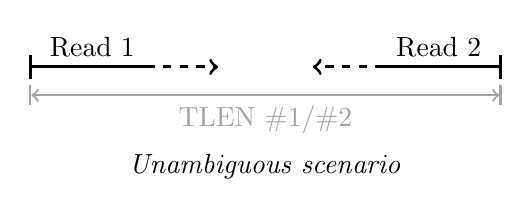
\begin{tikzpicture}[
    thick, xscale=2, yscale=1.8,
    read/.style={line width=0.4mm},
]
\draw[|-, read] (0,0)   -- (0.8,0)  node[midway, above] {Read 1};
\draw[->, read, dashed] (0.85,0) -- (1.2,0);
\draw[|-, read] (3,0) -- (2.2,0) node[midway, above] {Read 2};
\draw[->, read, dashed] (2.25,0) -- (1.8,0);
\draw[|<->|,gray!120]     (0,-.2) -- +(3,0) node[midway, below] {TLEN \#1/\#2};
\node at (1.5,-0.7) {\textit{Unambiguous scenario}};
\end{tikzpicture}
\hspace{3cm}% No space means side by side
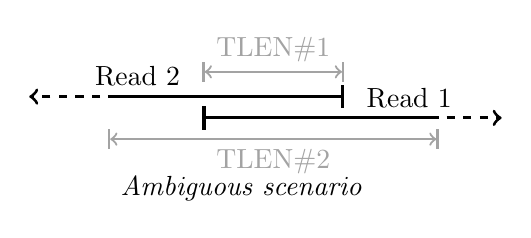
\begin{tikzpicture}[
    thick, xscale=1,yscale=0.9,
    read/.style={line width=0.4mm},
]
\draw[|-, read]         (2.2,0)   -- (5.2,0)    node[very near end, above] {Read 1};
\draw[->, read, dashed] (5.3,0)   -- (6,0);
\draw[-|, read]         (1,.3)    -- (4,.3)     node[very near start , above] {Read 2};
\draw[->, read, dashed] (0.9,.3)  -- (0,.3);
\draw[|<->|,gray!120]   (1,-0.3)  -- (5.2,-0.3) node[midway, below] {TLEN\#2};
\draw[|<->|,gray!120]   (2.2,0.65)-- (4,0.65)    node[midway, above] {TLEN\#1};
\node at (2.7,-1) {\textit{Ambiguous scenario}};
\end{tikzpicture}
\end{center}
}

\item {\sf SEQ}: segment SEQuence. This field can be a `*' when the
  sequence is not stored. If not a `*', the length of the sequence must
  equal the sum of lengths of {\tt M/I/S/=/X} operations in {\sf CIGAR}.
  An `=' denotes the base is identical to the reference base. No
  assumptions can be made on the letter cases.
\item {\sf QUAL}: ASCII of base QUALity plus 33 (same as the quality
  string in the Sanger FASTQ format). A base quality is the phred-scaled
  base error probability which equals $-10\log_{10}\Pr\{\mbox{base is
    wrong}\}$. This field can be a `*' when quality is not stored. If
  not a `*', {\sf SEQ} must not be a `*' and the length of the quality string
  ought to equal the length of {\sf SEQ}.
\end{enumerate}

\subsection{The alignment section: optional fields}\label{sec:alnaux}
All optional fields follow the {\tt TAG:TYPE:VALUE} format
where {\tt TAG} is a two-character string that matches {\tt /[A-Za-z][A-Za-z0-9]/}.
Each {\tt TAG} can only appear once in one alignment line. A {\tt TAG}
containing lowercase letters are reserved for end users.
In an optional field, {\tt TYPE} is a single case-sensitive letter which
defines the format of {\tt VALUE}:
\begin{center}\small
\begin{tabular}{cll}
\hline
{\bf Type} & {\bf Regexp matching {\tt VALUE}} & {\bf Description} \\
\hline
A & {\tt [!-\char126]} & Printable character \\
i & {\tt [-+]?[0-9]+} & Signed integer\footnotemark\\
f & {\tt [-+]?[0-9]*\char92.?[0-9]+([eE][-+]?[0-9]+)?} & Single-precision floating number \\
Z & {\tt [\,\,\,!-\char126]*} & Printable string, including space\\
H & {\tt ([0-9A-F][0-9A-F])*} & Byte array in the Hex format\footnotemark\\
B & {\tt [cCsSiIf](,[-+]?[0-9]*\char92.?[0-9]+([eE][-+]?[0-9]+)?)*} & Integer or numeric array\\
\hline
\end{tabular}
\addtocounter{footnote}{-1}
\footnotetext{The number of digits in an integer optional field is not
explicitly limited in SAM.  However, BAM can represent values in the
range~$[-2^{31},2^{32})$, so in practice this is the realistic range
of values for SAM's `{\tt i}' as well.}
\stepcounter{footnote}
\footnotetext{For example, the six-character Hex string `{\tt 1AE301}' represents the byte array $[{\tt 0x1a},{\tt 0xe3},{\tt 0x1}]$.}
\end{center}
For an integer or numeric array (type `{\tt B}'), the first letter indicates the type of numbers
in the following comma separated array. The letter can be one of `{\tt cCsSiIf}', corresponding to
{\tt int8\_t} (signed 8-bit integer), {\tt uint8\_t} (unsigned 8-bit integer), {\tt int16\_t}, {\tt uint16\_t}, {\tt int32\_t}, {\tt uint32\_t}
and {\tt float}, respectively.\footnotemark\@ During import/export, the element type
may be changed if the new type is also compatible with the array.
\footnotetext{Explicit typing eases format parsing and helps to reduce the file size when SAM is converted to BAM.}

Predefined tags are described in the separate {\sl Sequence Alignment/Map
Optional Fields Specification}.\footnote{See
\href{http://samtools.github.io/hts-specs/SAMtags.pdf}{\tt SAMtags.pdf}
at \url{https://github.com/samtools/hts-specs}.}
See that document for details of existing standard tag fields and conventions
around creating new tags that may be of general interest.
Tags starting with `{\tt X}', `{\tt Y}' or `{\tt Z}' and tags containing
lowercase letters in either position are reserved for local use and will
not be formally defined in any future version of these specifications.

\pagebreak

\section{Recommended Practice for the SAM Format}
\label{sec:recommended-practice}
This section describes the best practice for representing data in the
SAM format. They are not required in general, but may be required by a
specific software package for it to function properly.

\begin{enumerate}
\item The header section
  \begin{enumerate}[label=\arabic*]
  \item The {\tt @HD} line should be present, with either the {\tt SO} tag
    or the {\tt GO} tag (but not both) specified.
  \item The {\tt @SQ} lines should be present if reads have been mapped.
  \item When a {\tt RG} tag appears anywhere in the alignment section,
    there should be a single corresponding {\tt @RG} line with matching
    {\tt ID} tag in the header.
  \item When a {\tt PG} tag appears anywhere in the alignment section,
    there should be a single corresponding {\tt @PG} line with matching
    {\tt ID} tag in the header.
  \end{enumerate}
\item Adjacent CIGAR operations should be different.
\item No alignments should be assigned mapping quality 255.
\item Unmapped reads
  \begin{enumerate}[label=\arabic*]
  \item For a unmapped paired-end or mate-pair read whose mate is
    mapped, the unmapped read should have {\sf RNAME} and {\sf POS}
    identical to its mate.
  \item If all segments in a template are unmapped, their {\sf RNAME}
    should be set as `*' and {\sf POS} as 0.
  \item If {\sf POS} plus the sum of lengths of {\tt M/=/X/D/N}
    operations in {\sf CIGAR} exceeds the length specified in the {\tt
      LN} field of the {\tt @SQ} header line (if exists) with an SN
    equal to {\sf RNAME}, the alignment should be unmapped, unless the
    reference sequence is circular (see below).
  \item Unmapped reads should be stored in the orientation in which they came
    off the sequencing machine and have their {\sf reverse} flag bit~(0x10)
    correspondingly unset.
  \end{enumerate}
\item Multiple mapping
  \begin{enumerate}[label=\arabic*]
  \item When one segment is present in multiple lines to represent a multiple
	mapping of the segment, only one of these records should have the secondary
	alignment flag bit (0x100) unset. {\sf RNEXT} and {\sf PNEXT} point to the
	primary line of the next read in the template.
  \item {\sf SEQ} and {\sf QUAL} of secondary alignments should be set
    to `*' to reduce the file size.
  \end{enumerate}
%\item There should be no overlap between segments of a read\footnote{Few/no
%  existing aligners follow this practice.}.
\item Optional tags:
  \begin{enumerate}[label=\arabic*]
  \item If the template has more than 2 segments, the {\tt TC} tag
    should be present.
  \item The {\tt NM} tag should be present.
  \end{enumerate}

\item Circular reference sequences

Mappings that cross the coordinate `join' in circular reference sequences (i.e., those whose {\tt @SQ} headers specify {\tt TP:circular}) may be represented as follows:
  \begin{enumerate}[label=\arabic*]
  \item (Preferred)
As usual {\sf POS} should be between 1 and the {\tt @SQ} header's {\tt LN} value, but {\sf POS} plus the sum of the lengths of {\tt M/=/X/D/N} {\sf CIGAR} operations may exceed {\tt LN}.
Coordinates greater than~{\tt LN} are interpreted by subtracting {\tt LN} so that bases at $\texttt{LN}+1, \texttt{LN}+2, \texttt{LN}+3, \ldots$ are considered to be mapped at positions $1,2,3,\ldots$; thus each (1-based) position $p$ is interpreted as $((p-1)\bmod\texttt{LN})+1$.%
\footnote{The impact of this representation on indexing and random access is yet to be explored by implementations.}

  \item
Alternatively, such alignments may be split across several records: one record representing the initial portion of the segment ending at~{\tt LN}, one representing the final portion starting from~1, and any other records representing additional portions in between spanning the entire reference sequence.
One record (chosen arbitrarily) is considered primary and the remainder have their {\sf supplementary} flag bit (0x800) set.
  \end{enumerate}

\item Annotation dummy reads:
  These have {\sf SEQ} set to {\tt *}, {\sf FLAG} bits 0x100 and 0x200
  set (secondary and filtered), and a {\tt CT} tag.
  \begin{enumerate}[label=\arabic*]
%Repeating what is in the tag's footnote:
%  \item If the {\tt CT} tag's \emph{strand} is {\tt -}, FLAG bit 0x10
%  (reverse complemented) should be set, and otherwise not set.
  \item If you wish to store free text in a {\tt CT} tag, use the
  \emph{key} value {\tt Note} (uppercase N) to match GFF3.
  \item Multi-segment annotation (e.g., a gene with introns) should be
  described with multiple lines in SAM (like a multi-segment read).
  Where there is a clear biological direction (e.g., a gene), the first
  segment ({\sf FLAG} bit 0x40) is used for the first section (e.g., the
  $5'$ end of the gene). Thus a GenBank entry location like
  {\tt complement(join(85052..85354, 85441..85621, 86097..86284))}
  would have three lines in SAM with a common {\sf QNAME}: %And three lines in GFF3 too.
    \begin{center}\begin{tabular}{llrcl}
  & \multicolumn{1}{c}{\sf FLAG} & \multicolumn{1}{c}{\sf POS} & \sf CIGAR & \multicolumn{1}{c}{Optional fields} \\
The $5'$ fragment & 883 (0x373) & 86097 & \tt 188M & \tt FI:i:1\quad TC:i:3 \\
Middle fragment   & 819 (0x333) & 85441 & \tt 181M & \tt FI:i:2\quad TC:i:3 \\
The $3'$ fragment & 947 (0x3B3) & 85052 & \tt 303M & \tt FI:i:3\quad TC:i:3
    \end{tabular}\end{center}
  \item If converting GFF3 to SAM, store any \emph{key}, \emph{values}
  from column 9 in the {\tt CT} tag, except for the unique ID which
  is used for the QNAME. GFF3 columns 1 (seqid), 4 (start) and 5 (end)
  are encoded using SAM columns RNAME, POS and CIGAR to hold the length.
  GFF3 columns 3 (type) and 7 (strand) are stored explicitly in the
  {\tt CT} tag. Remaining GFF3 columns 2 (source), 6 (score), and
  8 (phase) are stored in the {\tt CT} tag using \emph{key} values
  {\tt FSource}, {\tt FScore} and {\tt FPhase} (uppercase keys are
  restricted in GFF3, so these names avoid clashes). Split location
  features are described with multiple lines in GFF3, and similarly
  become multi-segment dummy reads in SAM, with the {\sf RNEXT} and
  {\sf PNEXT} columns filled in appropriately. In the absence of a
  convention in SAM/BAM for reads wrapping the origin of a circular
  genome, any GFF3 feature line wrapping the origin must be split into
  two segments in SAM.
  \end{enumerate}
\end{enumerate}

\section{Guide for Describing Assembly Sequences in SAM}

\subsection{Unpadded versus padded representation}

To describe alignments, we can regard the reference sequence with no respect to
other alignments against it.  Such a reference sequence is called an
\emph{unpadded reference}. A position on an unpadded reference, referred to
as an \emph{unpadded position}, is not affected by any alignments. When we use
unpadded references and positions to describe alignments, we say we are using
the \emph{unpadded representation}.

Alternatively, to describe the same alignments, we can modify the reference
sequence to contain pads that make room for sequences inserted relative to the
reference. A pad is effectively a gap and conventionally represented by an
asterisk `*'.  A reference sequence containing pads is called a \emph{padded
reference}. A position which counts the *'s is referred to as a \emph{padded
position}. A padded reference sequence may be affected by the query alignments
and because of gap insertions is typically longer than the unpadded reference.
The padded position of one query alignment may be affected by other query
alignments.

Unpadded and padded are different representations of the same alignments. They
are convertible to each other with no loss of any information. The unpadded
representation is more common due to the convenience of a fixed coordinate system,
while the padded representation has the advantage that alignments can be simply
described by the start and end coordinates without using complex CIGAR strings.
SAM traditionally uses the padded representation for {\it de novo} assembly.
The ACE assembly format uses the padded representation exclusively.

\subsection{Padded SAM}\label{sec:padded-sam}

The SAM format is typically used to describe alignments against an unpadded
reference sequence, but it is also able to describe alignments against a padded
reference. In the latter case, we say we are using a \emph{padded SAM}. A padded
SAM is a valid SAM, but with the difference that the reference and positions in
use are padded. There may be more than one way to describe the padded
representation.
We recommend the following; see also the discussion in Cock {\it et al.}%
\footnote{Peter J. A. Cock, James K. Bonfield, Bastien Chevreux, and Heng Li,
{\bf SAM/BAM format v1.5 extensions for \emph{de novo} assemblies},
{\sl bioRxiv 020024};
\href{http://dx.doi.org/10.1101/020024}{doi:10.1101/020024}.}

In a padded SAM, alignments and coordinates are described with respect to the
padded reference sequence. Unlike traditional padded representations like
the ACE file format where pads/gaps are recorded in reads using *'s, we do
not write *'s in the {\sf SEQ} field of the SAM format.\footnote{Writing
pads/gaps as *'s in the {\sf SEQ} field might have been more convenient, but
this caused concerns for backward compatibility.} Instead, we describe pads
in the query sequences as deletions from the padded reference using the
{\sf CIGAR} `{\tt D}' operation. In a padded SAM, the insertion and padding
CIGAR operations (`{\tt I}' and `{\tt P}') are not used because the padded
reference already considers all the insertions.

The following shows the padded SAM for the example alignment in Section~\ref{sec:example}.
Notably, the length of {\tt ref} is 47 instead of 45. {\sf POS} of the last
three alignments are all shifted by 2. {\sf CIGAR} of alignments bridging the
2bp insertion are also changed.

\begin{framed}\small
\begin{verbatim}
@HD VN:1.6 SO:coordinate
@SQ SN:ref LN:47
ref   516 ref  1  0 14M2D31M   *  0   0 AGCATGTTAGATAAGATAGCTGTGCTAGTAGGCAGTCAGCGCCAT *
r001   99 ref  7 30 14M1D3M    = 39  41 TTAGATAAAGGATACTG *
*     768 ref  8 30 1M         *  0   0 *                 * CT:Z:.;Warning;Note=Ref wrong?
r002    0 ref  9 30 3S6M1D5M   *  0   0 AAAAGATAAGGATA    * PT:Z:1;4;+;homopolymer
r003    0 ref  9 30 5H6M       *  0   0 AGCTAA            * NM:i:1
r004    0 ref 18 30 6M14N5M    *  0   0 ATAGCTTCAGC       *
r003 2064 ref 31 30 6H5M       *  0   0 TAGGC             * NM:i:0
r001  147 ref 39 30 9M         =  7 -41 CAGCGGCAT         * NM:i:1
\end{verbatim}
\end{framed}

Here we also exemplify the recommended practice for storing the reference
sequence and the reference annotations in SAM when necessary. For a reference
sequence in SAM, {\sf QNAME} should be identical to {\sf RNAME}, {\sf POS} set
to 1 and {\sf FLAG} to 516 (filtered and unmapped); for an annotation, {\sf
FLAG} should be set to 768 (filtered and secondary) with no restriction to {\sf
QNAME}.
Dummy reads for annotation would typically have a {\tt CT} tag to hold the annotation information; see the discussion of dummy reads in Section~\ref{sec:recommended-practice}.
See also the separate {\sl Optional Fields Specification} for full details of the {\tt CT} and {\tt PT} annotation tags.%
\footnote{See \emph{Annotation and Padding} in \href{http://samtools.github.io/hts-specs/SAMtags.pdf}{\tt SAMtags.pdf}.}

\pagebreak

\section{The BAM Format Specification}

\subsection{The BGZF compression format}

BGZF is block compression implemented on top of the standard gzip file
format.\footnote{L.~Peter Deutsch, {\bf GZIP file format specification
version~4.3}, \href{http://tools.ietf.org/html/rfc1952}{\sl RFC 1952}.}
The goal of BGZF is to provide good compression while allowing
efficient random access to the BAM file for indexed queries. The BGZF
format is `gunzip compatible', in the sense that a compliant gunzip
utility can decompress a BGZF compressed file.\footnote{It is worth noting that there is a known bug in the Java {\sf
  GZIPInputStream} class that concatenated gzip archives cannot be
successfully decompressed by this class. BGZF files can be created and
manipulated using the built-in Java {\sf util.zip} package, but naive
use of {\sf GZIPInputStream} on a BGZF file will not work due to this
bug.}

A BGZF file is a series of concatenated BGZF blocks, each no larger
than~64Kb before or after compression. Each BGZF block
is itself a spec-compliant gzip archive which contains an ``extra field''
in the format described in RFC1952. The gzip file format allows the
inclusion of application-specific extra fields and these are ignored by
compliant decompression implementation. The gzip specification also
allows gzip files to be concatenated. The result of decompressing
concatenated gzip files is the concatenation of the uncompressed data.

Each BGZF block contains a standard gzip file header with the following
standard-compliant extensions:

\begin{enumerate}
\item The {\sf F.EXTRA} bit in the header is set to indicate that extra
  fields are present.
\item The extra field used by BGZF uses the two subfield ID values 66 and 67 (ascii `BC').
\item The length of the BGZF extra field payload (field {\sf LEN} in the
  gzip specification) is 2 (two bytes of payload).
\item The payload of the BGZF extra field is a 16-bit unsigned integer
  in little endian format. This integer gives the size of the containing
  BGZF block minus one.
\end{enumerate}

On disk, a complete BGZF file is a series of blocks as shown in the following
table.  (All integers are little endian as is required by RFC1952.)
\begin{table}[ht]
\centering
{\small
\begin{tabular}{|l|l|l|l|l|r|}
  \cline{1-6}
  \multicolumn{3}{|c|}{\bf Field} & \multicolumn{1}{c|}{\bf Description} & \multicolumn{1}{c|}{\bf Type} & \multicolumn{1}{c|}{\bf Value} \\\cline{1-6}
  \multicolumn{6}{|c|}{\textcolor{gray}{\it List of compression blocks (until the end of the file)}} \\\cline{2-6}
  & \multicolumn{2}{l|}{\sf ID1} & gzip IDentifier1 & {\tt uint8\_t} & 31 \\\cline{2-6}
  & \multicolumn{2}{l|}{\sf ID2} & gzip IDentifier2 & {\tt uint8\_t} & 139 \\\cline{2-6}
  & \multicolumn{2}{l|}{\sf CM} & gzip Compression Method & {\tt uint8\_t} & 8 \\\cline{2-6}
  & \multicolumn{2}{l|}{\sf FLG} & gzip FLaGs & {\tt uint8\_t} & 4 \\\cline{2-6}
  & \multicolumn{2}{l|}{\sf MTIME} & gzip Modification TIME & {\tt uint32\_t} & \\\cline{2-6}
  & \multicolumn{2}{l|}{\sf XFL} & gzip eXtra FLags & {\tt uint8\_t} & \\\cline{2-6}
  & \multicolumn{2}{l|}{\sf OS} & gzip Operating System & {\tt uint8\_t} & \\\cline{2-6}
  & \multicolumn{2}{l|}{\sf XLEN} & gzip eXtra LENgth & {\tt uint16\_t} & \\\cline{2-6}
  & \multicolumn{5}{c|}{\textcolor{gray}{\it Extra subfield(s) (total size=XLEN)}} \\\cline{3-6}
  & & \multicolumn{4}{c|}{\textcolor{gray}{\it Additional RFC1952 extra subfields if present}} \\\cline{3-6}
  & & {\sf SI1} & Subfield Identifier1 & {\tt uint8\_t} & 66 \\\cline{3-6}
  & & {\sf SI2} & Subfield Identifier2 & {\tt uint8\_t} & 67 \\\cline{3-6}
  & & {\sf SLEN} & Subfield LENgth & {\tt uint16\_t} & 2 \\\cline{3-6}
  & & {\sf BSIZE} & total Block SIZE minus 1 & {\tt uint16\_t} & \\\cline{3-6}
  & & \multicolumn{4}{c|}{\textcolor{gray}{\it Additional RFC1952 extra subfields if present}} \\\cline{2-6}
  & \multicolumn{2}{l|}{\sf CDATA} & Compressed DATA by {\sf zlib::deflate()} & {\tt uint8\_t[{\sf BSIZE-XLEN-19}]} & \\\cline{2-6}
  & \multicolumn{2}{l|}{\sf CRC32} & CRC-32 & {\tt uint32\_t} & \\\cline{2-6}
  & \multicolumn{2}{l|}{\sf ISIZE} & Input SIZE (length of uncompressed data) & {\tt uint32\_t} & \\
  \cline{1-6}
\end{tabular}}
\end{table}

The random access method to be described next limits the uncompressed
contents of each BGZF block to a maximum of $2^{16}$~bytes of data.
Thus while {\sf ISIZE} is stored as a {\tt uint32\_t} as per the gzip format,
in BGZF it is limited to the range~$[0,65536]$.
{\sf BSIZE} can represent BGZF block sizes in the range~$[1,65536]$, though
typically {\sf BSIZE} will be rather less than~{\sf ISIZE} due to compression.

\subsubsection{Random access}

BGZF files support random access through the BAM file index. To achieve
this, the BAM file index uses \emph{virtual file offsets} into the BGZF
file. Each virtual file offset is an unsigned 64-bit integer, defined as: {\tt
  coffset\char60\char60 16\char124uoffset}, where {\tt coffset} is an
unsigned byte offset into the BGZF file to the beginning of a BGZF
block, and {\tt uoffset} is an unsigned byte offset into the
uncompressed data stream represented by that BGZF block. Virtual file
offsets can be compared, but subtraction between virtual file offsets
and addition between a virtual offset and an integer are both
disallowed.

\subsubsection{End-of-file marker}

An end-of-file (EOF) trailer or marker block should be written at the end
of BGZF files, so that unintended file truncation can be easily detected.
The EOF marker block is a particular empty\footnotemark\ BGZF block
encoded with the default {\sf zlib} compression level settings,
and consists of the following 28~hexadecimal bytes:
\begin{center}
\texttt{1f 8b 08 04 00 00 00 00 00 ff 06 00 42 43 02 00 1b 00 03 00 00 00 00 00 00 00 00 00}
\end{center}

\footnotetext{Empty in the sense of having been formed by compressing
a data block of length zero.}

\noindent
The presence of this EOF marker at the end of a BGZF file indicates that the
immediately following physical EOF is the end of the file as intended by the
program that wrote it.
Empty BGZF blocks are not otherwise special; in particular, the presence of
an EOF marker block does not by itself signal end of file.\footnotemark

\footnotetext{An implementation that supports reopening a BAM file in append
mode could produce a file by writing headers and alignment records to it,
closing it (adding an EOF marker); then reopening it for append, writing
more alignment records, and closing it (adding an EOF marker).
The resulting BAM file would contain an embedded insignificant EOF~marker
block that should be effectively ignored when it is read.}

The absence of this final EOF marker should trigger a warning or error
soon after opening a BGZF file where random access is available.\footnotemark\
When reading a BGZF file in sequential streaming fashion, ideally this
EOF check should be performed when the end of the stream is reached.
Checking that the final BGZF block in the file decompresses to empty
or checking that the last 28 bytes of the file are exactly the bytes
above are both sufficient tests; each is likely more convenient in
different circumstances.

\footnotetext{It is useful to produce a diagnostic at the beginning of
reading a file, so that interactive users can abort lengthy analysis of
potentially-corrupted files.  Of course, this is only possible if the
stream in question supports random access.}

\pagebreak

\subsection{The BAM format}
BAM is compressed in the BGZF format. All multi-byte numbers in BAM are
little-endian, regardless of the machine endianness. The format is
formally described in the following table where values in brackets are
the default when the corresponding information is not available; an
underlined word in uppercase denotes a field in the SAM format.

\begin{table}[ht]
\centering
{\small
\begin{tabular}{|l|l|l|p{8.15cm}|l|r|}
  \cline{1-6}
  \multicolumn{3}{|c|}{\bf Field} & \multicolumn{1}{c|}{\bf Description} & \multicolumn{1}{c|}{\bf Type} & \multicolumn{1}{c|}{\bf Value} \\\cline{1-6}
  \multicolumn{3}{|l|}{\sf magic} & BAM magic string & {\tt char[4]} & {\tt BAM\char92 1}\\\cline{1-6}
  \multicolumn{3}{|l|}{\sf l\_text} & Length of the header text, including any {\tt NUL} padding & {\tt uint32\_t} & $< 2^{31}$ \\\cline{1-6}
  \multicolumn{3}{|l|}{\sf text} & Plain header text in SAM; not necessarily {\tt NUL}-terminated & {\tt char[{\sf l\_text}]} & \\\cline{1-6}
  % Pedantically this should be <= but we restrict |refs| by one so n_ref fits in a signed 32-bit int.
  \multicolumn{3}{|l|}{\sf n\_ref} & \# reference sequences & {\tt uint32\_t} & $< 2^{31}$ \\\cline{1-6}
  \multicolumn{6}{|c|}{\textcolor{gray}{\it List of reference information (n=n\_ref)}} \\\cline{2-6}
  & \multicolumn{2}{l|}{\sf l\_name} & Length of the reference name plus 1 (including {\tt NUL}) & {\tt uint32\_t} & \memlimited \\\cline{2-6}
  & \multicolumn{2}{l|}{\sf name} & Reference sequence name; {\tt NUL}-terminated & {\tt char[{\sf l\_name}]} & \\\cline{2-6}
  & \multicolumn{2}{l|}{\sf l\_ref} & Length of the reference sequence & {\tt uint32\_t} & $< 2^{31}$ \\\cline{1-6}
  \multicolumn{6}{|c|}{\textcolor{gray}{\it List of alignments (until the end of the file)}} \\\cline{2-6}
  & \multicolumn{2}{l|}{\sf block\_size} & Total length of the alignment record, excluding this field & {\tt uint32\_t} & \memlimited \\\cline{2-6}
  & \multicolumn{2}{l|}{\sf refID} & Reference sequence ID, $-1\leq{\sf refID}<{\sf n\_ref}$; -1 for a read without a mapping position & {\tt int32\_t} & [-1] \\\cline{2-6}
  & \multicolumn{2}{l|}{\sf pos} & 0-based leftmost coordinate ($=\underline{\sf POS}-1$)& {\tt int32\_t} & [-1]\\\cline{2-6}
  & \multicolumn{2}{l|}{\sf l\_read\_name} & Length of {\sf read\_name} below ($={\sf length}(\underline{\sf QNAME})+1$) & {\tt uint8\_t} & \\\cline{2-6}
  & \multicolumn{2}{l|}{\sf mapq} & Mapping quality (=\underline{\sf MAPQ}) & {\tt uint8\_t} & \\\cline{2-6}
  & \multicolumn{2}{l|}{\sf bin} & BAI index bin, see Section~\ref{sec:bin-field}  & {\tt uint16\_t} & \\\cline{2-6}
  & \multicolumn{2}{l|}{\sf n\_cigar\_op} & Number of operations in \underline{\sf CIGAR}, see Section~\ref{sec:ncigar} & {\tt uint16\_t} & \\\cline{2-6}
  & \multicolumn{2}{l|}{\sf flag} & Bitwise flags (= \underline{\sf FLAG})\footnotemark\ & {\tt uint16\_t} & \\\cline{2-6}
  & \multicolumn{2}{l|}{\sf l\_seq} & Length of \underline{\sf SEQ} & {\tt uint32\_t} & \memlimited \\\cline{2-6}
  & \multicolumn{2}{l|}{\sf next\_refID} & Ref-ID of the next segment ($-1\le{\sf next\_refID}<{\sf n\_ref}$) & {\tt int32\_t} & [-1] \\\cline{2-6}
  & \multicolumn{2}{l|}{\sf next\_pos} & 0-based leftmost pos of the next segment ($=\underline{\sf PNEXT}-1$) & {\tt int32\_t} & [-1] \\\cline{2-6}
  & \multicolumn{2}{l|}{\sf tlen} & Template length ($=\underline{\sf TLEN}$) & {\tt int32\_t} & [0] \\\cline{2-6}
  & \multicolumn{2}{l|}{\sf read\_name} & Read name, {\tt NUL}-terminated (\underline{\sf QNAME} with trailing `{\tt\verb"\0"}')\footnotemark & {\tt char[{\sf l\_read\_name}]} & \\\cline{2-6}
  & \multicolumn{2}{l|}{\sf cigar} & CIGAR: {\tt {\sf op\_len}\char60\char60 4\char124{\sf op}}. `{\tt MIDNSHP\char61X}'$\to$`012345678' & {\tt uint32\_t[{\sf n\_cigar\_op}]} & \\\cline{2-6}
  & \multicolumn{2}{l|}{\sf seq} & 4-bit encoded read: `{\tt =ACMGRSVTWYHKDBN}'$\to[0,15]$. See Section~\ref{sec:seq} & {\tt uint8\_t[({\sf l\_seq}+1)/2]} & \\\cline{2-6}
  & \multicolumn{2}{l|}{\sf qual} & Phred-scaled base qualities. See Section~\ref{sec:seq} & {\tt char[{\sf l\_seq}]} & \\\cline{2-6}
  & \multicolumn{5}{c|}{\textcolor{gray}{\it List of auxiliary data (until the end of the alignment block)}} \\\cline{3-6}
  & & {\sf tag} & Two-character tag & {\tt char[2]} & \\\cline{3-6}
  & & {\sf val\_type} & Value type: {\tt AcCsSiIfZHB}, see Section~\ref{sec:aux-type-codes} & {\tt char} & \\\cline{3-6}
  & & {\sf value} & Tag value & (by {\sf val\_type}) &\\
  \cline{1-6}
\end{tabular}}
\end{table}
\addtocounter{footnote}{-1}
\footnotetext{As noted in Section~\ref{sec:alnrecord}, reserved {\sf FLAG} bits
should be written as zero and ignored on reading by current software.}
\stepcounter{footnote}
\footnotetext{For backward compatibility, an absent {\sf QNAME} (represented as `{\tt *}' in SAM) is stored as a C string {\tt "*\char92 0"}.}

\noindent
Most length and count fields described as {\tt uint32\_t} have additional constraints on their range:
$\mbox{\sf l\_text} < 2^{31}$ due to implementation limits;
$\mbox{\sf n\_ref} < 2^{31}$ because {\sf refID} and {\sf next\_refID} are signed;
$\mbox{\sf l\_ref} < 2^{31}$ because {\sf tlen} is signed;
those marked ``\textit{limited}'' are limited by available memory and the practical size of the data represented well before they are limited by, e.g., Java's signed 32-bit integer maximum array size.

\subsubsection{BIN field calculation}\label{sec:bin-field}
{\sf BIN} is calculated using the {\sf reg2bin()} function in
Section~\ref{sec:code}.
For mapped reads this uses {\sf POS-1} (i.e.,~0-based left position) and the
alignment end point using the alignment length from the {\sf CIGAR} string.
For unmapped reads (e.g.,~paired end reads where only one part is mapped, see
Section~\ref{sec:recommended-practice}) the alignment is treated as
being length one.
Note unmapped reads with {\sf POS} $0$ (which becomes $-1$ in BAM) therefore
use {\sf reg2bin(-1, 0)} which is $4680$.

\subsubsection{N\_CIGAR\_OP field}\label{sec:ncigar}
With 16 bits, {\sf n\_cigar\_op} can keep at most 65535 CIGAR
operations in BAM files. For an alignment with more CIGAR operations, BAM
stores the real {\sf CIGAR}, encoded the same way as the {\sf cigar} field in
BAM, in the {\tt CG} optional tag of type `{\tt B,I}', and sets {\sf CIGAR} to
`\textit{k}{\tt S}\textit{m}{\tt N}' as a placeholder, where `\textit{k}' equals {\sf l\_seq}, `\textit{m}'
is the reference sequence length in the alignment, and `{\tt S}' and `{\tt N}'
are the soft-clipping and reference-clip CIGAR operators, respectively---i.e.,
in the binary form, {\sf n\_cigar\_op}=2 and {\sf cigar}={\tt [\textit{k}\char60\char60
4\char124{4},\textit{m}\char60\char60 4\char124{3}]}. If tag {\tt CG} is present and
the first CIGAR operation clips the entire read, a BAM parsing library is
expected to update {\sf n\_cigar\_op} and {\sf cigar} with the real CIGAR
stored in the {\tt CG} tag and remove the now-redundant {\tt CG} tag.

\subsubsection{SEQ and QUAL encoding}\label{sec:seq}
Sequence is encoded in 4-bit values, with adjacent bases packed into the same byte starting with the highest 4 bits first.
When {\sf l\_seq} is odd the bottom 4 bits of the last byte are undefined, but we recommend writing these as zero.
The case-insensitive base codes `{\tt =ACMGRSVTWYHKDBN}' are mapped to $[0,15]$ respectively with all other characters mapping to `{\tt N}' (value 15).

Omitted sequence, represented in SAM as `{\tt *}', is represented by {\sf l\_seq} being 0 and {\sf seq} and {\sf qual} zero-length.

Base qualities are stored as bytes in the range $[0,93]$, without any +33 conversion to printable ASCII.
When base qualities are omitted but the sequence is not, {\sf qual} is filled with {\tt 0xFF} bytes (to length {\sf l\_seq}).

\subsubsection{Auxiliary data encoding}\label{sec:aux-type-codes}
Optional alignment fields are stored immediately after each other immediately
following the {\sf qual} field, and are included in {\sf block\_size}.
Each field is represented as a two-character tag followed by a single type
character and then its value, whose length is determined by the field's type.

\newcommand*{\tagfield}[2]{\firstbytebox{2}{\em tag}\bytebox{1}{\tt #1}#2}

Single character `{\tt A}' fields have a total length of 4~bytes,
with the value represented as a single byte:
\begin{center}\small\byteboxsetup
\tagfield{A}{\bytebox{1}{char}}
\end{center}

While all single (i.e., non-array) integer types are stored in SAM as `{\tt i}',
in BAM any of `{\tt cCsSiI}' may be used together with the correspondingly-sized
binary integer value, chosen according to the field value's magnitude.%
\footnote{The signedness and size used for each integer value is an
implementation choice, but is typically the smallest that suffices.}
Similarly floating point `{\tt f}' fields are represented as IEEE 754-2008
binary32 values.
Thus BAM numeric fields have a total length of~4, 5, or~7~bytes:
\begin{center}\small\byteboxsetup\begin{tabular}{l@{\hspace{1in}}l}
\tagfield{c}{\bytebox{1}{i8}} \quad (i.e., {\tt int8\_t})
    & \tagfield{i}{\bytebox{4}{int32\_t}} \\
\tagfield{C}{\bytebox{1}{u8}} \quad (i.e., {\tt uint8\_t})
    & \tagfield{I}{\bytebox{4}{uint32\_t}} \\
\tagfield{s}{\bytebox{2}{int16\_t}}
    & \tagfield{f}{\bytebox{4}{float}} \\
\tagfield{S}{\bytebox{2}{uint16\_t}}
    &
\end{tabular}\end{center}

\newcommand*{\byteboxvector}[2]{\bytebox{#1}{#2}\bytebox{#1}{#2}\makebox[1.5\bytewidth][c]{$\cdots$}\firstbytebox{#1}{#2}}

String fields and hex-formatted byte arrays are represented as
{\tt NUL}-terminated text strings:%
\footnote{The BAM representation of `{\tt H}' field values as textual
hexadecimal digits rather than binary data is for historical reasons.
Modern applications may prefer to use `{\tt B,C}' array fields rather
than `{\tt H}' fields.}
\begin{center}\small\byteboxsetup\begin{tabular}{l}
\tagfield{Z}{\byteboxvector{1}{char}\bytebox{1}{\tt NUL}} \\
\tagfield{H}{\byteboxvector{2}{hex hex}\bytebox{1}{\tt NUL}}
\end{tabular}\end{center}

\newcommand*{\arraytagfield}[3]{\tagfield{B}{\bytebox{1}{\tt #1}\bytebox{4}{\em count}\byteboxvector{#2}{#3}}}

\begin{samepage}
The representation of a `{\tt B}' array field starts with a sub-type character
similar to the numeric field types above and a \emph{count} ({\tt uint32\_t}, but
limited by memory and {\sf block\_size}) giving the number of elements in the array.
The array elements follow, encoded as binary integers or IEEE floats sized
according to the sub-type:
\begin{center}\small\byteboxsetup\begin{tabular}{l}
\arraytagfield{c}{1}{i8} \quad (i.e., {\tt int8\_t} elements) \\
\arraytagfield{C}{1}{u8} \quad (i.e., {\tt uint8\_t} elements) \\
\arraytagfield{s}{2}{int16\_t} \\
\arraytagfield{S}{2}{uint16\_t} \\
\arraytagfield{i}{4}{int32\_t} \\
\arraytagfield{I}{4}{uint32\_t} \\
\arraytagfield{f}{4}{float}
\end{tabular}\end{center}
\end{samepage}

\pagebreak

\section{Indexing BAM}
Indexing aims to achieve fast retrieval of alignments overlapping a
specified region without going through the whole alignments. BAM must be
sorted by the reference ID and then the leftmost coordinate before
indexing.

This section describes the binning scheme underlying coordinate-sorted
BAM indices and its implementation in the long-established BAI format.
The CSI format documented elsewhere uses a similar binning scheme and
can also be used to index BAM.\footnotemark

\footnotetext{See \href{http://samtools.github.io/hts-specs/CSIv1.pdf}
{\tt CSIv1.pdf} at \url{https://github.com/samtools/hts-specs}.
This is a separate specification because CSI is also used to index other
coordinate-sorted file formats in addition to BAM.}

\subsection{Algorithm}
\subsubsection{Basic binning index}
The UCSC binning scheme was suggested by Richard Durbin and Lincoln Stein
and is explained in Kent {\it et al.}\footnotemark\ In this scheme, each bin
represents a contiguous genomic region which is either fully contained
in or non-overlapping with another bin; each alignment is associated
with a bin which represents the smallest region containing the entire
alignment. The binning scheme is essentially a representation of
R-tree. A distinct bin uniquely corresponds to a distinct internal node
in a R-tree. Bin A is a child of Bin B if the region represented by A is
contained in B.

\footnotetext{W.~James Kent {\it et al.},
{\bf The Human Genome Browser at UCSC}, {\sl Genome Res.}~2002~12: 996--1006;
\href{http://dx.doi.org/doi:10.1101/gr.229102}{doi:10.1101/\linebreak[1]gr.229102};
{\sc pmid:}12045153.  See in particular {\sl The Database}, p1003.}

To find the alignments that overlap a specified region, we need to get
the bins that overlap the region, and then test each alignment in the
bins to check overlap. To quickly find alignments associated with a
specified bin, we can keep in the index the start file offsets of chunks
of alignments which all have the bin. As alignments are sorted by the
leftmost coordinates, alignments having the same bin tend to be
clustered together on the disk and therefore usually a bin is only
associated with a few chunks. Traversing all the alignments having the
same bin usually needs a few seek calls. Given the set of bins that
overlap the specified region, we can visit alignments in the order of
their leftmost coordinates and stop seeking the rest when an alignment
falls outside the required region. This strategy saves half of the seek
calls in average.

In the BAI format, each bin may span $2^{29}$, $2^{26}$, $2^{23}$, $2^{20}$,
$2^{17}$ or $2^{14}$ bp. Bin 0 spans a 512Mbp region, bins 1--8 span 64Mbp,
9--72 8Mbp, 73--584 1Mbp, 585--4680 128Kbp, and bins 4681--37448 span 16Kbp
regions.  This implies that this index format does not support reference
chromosome sequences longer than $2^{29}-1$.

The CSI format generalises the sizes of the bins, and supports reference
sequences of the same length as are supported by SAM and BAM.

\subsubsection{Reducing small chunks}
Around the boundary of two adjacent bins, we may see many small chunks
with some having a shorter bin while the rest having a larger bin. To
reduce the number of seek calls, we may join two chunks having the same
bin if they are close to each other. After this process, a joined chunk
will contain alignments with different bins. We need to keep in the
index the file offset of the end of each chunk to identify its
boundaries.

\subsubsection{Combining with linear index}
For an alignment starting beyond 64Mbp, we always need to seek to some
chunks in bin 0, which can be avoided by using a linear index. In the
linear index, for each tiling 16384bp window on the reference, we record
the smallest file offset of the alignments that overlap with the
window. Given a region [rbeg,\,rend), we only need to visit a chunk whose
end file offset is larger than the file offset of the 16kbp window
containing rbeg.

With both binning and linear indices, we can retrieve alignments in most
of regions with just one seek call.

\subsubsection{A conceptual example}
Suppose we have a genome shorter than 144kbp. We can design a binning
scheme which consists of three types of bins: bin 0 spans 0-144kbp, bin
1, 2 and 3 span 48kbp and bins from 4 to 12 span 16kbp each:

\begin{table}[ht]
  \centering
  {\small\begin{tabular}{|c|c|c|c|c|c|c|c|c|}
    \cline{1-9}
    \multicolumn{9}{|c|}{0 (0--144kbp)}\\\cline{1-9}
    \multicolumn{3}{|c|}{1 (0--48kbp)} & \multicolumn{3}{c|}{2 (48--96kbp)} & \multicolumn{3}{c|}{3 (96--144kbp)} \\\cline{1-9}
    4 (0--16k) & 5 (16--32k) & 6 (32--48k) & 7 (48--64k) & 8 (64--80k) & 9 (80--96k) & 10 & 11 & 12 \\
    \cline{1-9}
  \end{tabular}}
\end{table}

An alignment starting at 65kbp and ending at 67kbp would have a bin
number 8, which is the smallest bin containing the alignment. Similarly,
an alignment starting at 51kbp and ending at 70kbp would go to bin 2,
while an alignment between [40k,\,49k] to bin 0. Suppose we want to find
all the alignments overlapping region [65k,\,71k). We first calculate that
bin 0, 2 and 8 overlap with this region and then traverse the alignments
in these bins to find the required alignments. With a binning index
alone, we need to visit the alignment at [40k,\,49k] as it belongs to bin
0. But with a linear index, we know that such an alignment stops before
64kbp and cannot overlap the specified region. A seek call can thus be
saved.

\subsection{The BAI index format for BAM files}
\begin{table}[ht]
\centering\small
\begin{tabular}{|l|l|l|l|l|l|r|}
  \cline{1-7}
  \multicolumn{4}{|c|}{\bf Field} & \multicolumn{1}{c|}{\bf Description} & \multicolumn{1}{c|}{\bf Type} & \multicolumn{1}{c|}{\bf Value} \\\cline{1-7}
  \multicolumn{4}{|l|}{\sf magic} & Magic string & {\tt char[4]} & {\tt BAI\char92 1}\\\cline{1-7}
  \multicolumn{4}{|l|}{\sf n\_ref} & \# reference sequences & {\tt uint32\_t} & $< 2^{31}$ \\\cline{1-7}
  \multicolumn{7}{|c|}{\textcolor{gray}{\it List of indices (n=n\_ref)}} \\\cline{2-7}
  & \multicolumn{3}{l|}{\sf n\_bin} & \# distinct bins (for the binning index) & {\tt uint32\_t} & $\le 37451$ \\\cline{2-7}
  & \multicolumn{6}{c|}{\textcolor{gray}{\it List of distinct bins (n=n\_bin)}} \\\cline{3-7}
  & & \multicolumn{2}{l|}{\sf bin} & Distinct bin & {\tt uint32\_t} & $\le 37450$ \\\cline{3-7}
  & & \multicolumn{2}{l|}{\sf n\_chunk} & \# chunks & {\tt uint32\_t} & \memlimited\footnotemark \\\cline{3-7}
  & & \multicolumn{5}{c|}{\textcolor{gray}{\it List of chunks (n=n\_chunk)}} \\\cline{4-7}
  & & & {\sf chunk\_beg} & (Virtual) file offset of the start of the chunk & {\tt uint64\_t} & \\\cline{4-7}
  & & & {\sf chunk\_end} & (Virtual) file offset of the end of the chunk & {\tt uint64\_t} & \\\cline{2-7}
  & \multicolumn{3}{l|}{\sf n\_intv} & \# 16kbp intervals (for the linear index) & {\tt uint32\_t} & $\le 2^{17}$ \\\cline{2-7}
  & \multicolumn{6}{c|}{\textcolor{gray}{\it List of intervals (n=n\_intv)}} \\\cline{3-7}
  & & \multicolumn{2}{l|}{\sf ioffset} & (Virtual) file offset of the first alignment in the interval & {\tt uint64\_t} & \\\cline{1-7}
  \multicolumn{4}{|l|}{{\sf n\_no\_coor} (optional)} & Number of unplaced unmapped reads ({\sf RNAME} *) & {\tt uint64\_t} & \\\cline{1-7}
\end{tabular}
\end{table}

\footnotetext{The number of chunks in a single bin is effectively limited by available memory and in any case is typically a maximum of some thousands.}

The index file may optionally contain additional metadata providing a summary
of the number of mapped and unmapped read-segments per reference sequence,
and of any unplaced unmapped read-segments.\footnote{By \emph{placed unmapped
read} we mean a read that is unmapped according to its {\sf FLAG} but whose
{\sf RNAME} and~{\sf POS} fields are filled in, thus ``placing'' it on a
reference sequence (see Section~\ref{sec:recommended-practice}).
In contrast, \emph{unplaced} unmapped reads have~`*' and~0 for {\sf RNAME}
and~{\sf POS}.}
This is stored in an optional extra metadata pseudo-bin for each reference
sequence, and in the optional trailing {\sf n\_no\_coor} field at the end of
the file.

The pseudo-bins appear in the references' lists of distinct bins as bin
number~37450 (which is beyond the normal range) and are laid out so as to be
compatible with real bins and their chunks:

\begin{table}[ht]
\centering\small
\begin{tabular}{|l|l|l|r|}
  \hline
  {\sf bin} & Magic bin number & {\tt uint32\_t} & 37450 \\\hline
  {\sf n\_chunk} & \# chunks & {\tt uint32\_t} & 2 \\\hline
  {\sf unmapped\_beg} & (Virtual) file offset of the start of placed unmapped reads & {\tt uint64\_t} & \\\hline
  {\sf unmapped\_end} & (Virtual) file offset of the end of placed unmapped reads & {\tt uint64\_t} & \\\hline
  {\sf n\_mapped} & Number of mapped read-segments for this reference & {\tt uint64\_t} & \\\hline
  {\sf n\_unmapped} & Number of unmapped read-segments for this reference & {\tt uint64\_t} & \\\hline
\end{tabular}
\end{table}

\subsection{C source code for computing bin number and overlapping bins}\label{sec:code}
The following functions compute bin numbers and overlaps for a BAI-style
binning scheme with $6$~levels and a minimum bin size of $2^{14}$~bp.
See the CSI specification for generalisations of these functions designed for
binning schemes with arbitrary depth and sizes.

{\small
\begin{verbatim}
/* calculate bin given an alignment covering [beg,end) (zero-based, half-closed-half-open) */
int reg2bin(int beg, int end)
{
    --end;
    if (beg>>14 == end>>14) return ((1<<15)-1)/7 + (beg>>14);
    if (beg>>17 == end>>17) return ((1<<12)-1)/7 + (beg>>17);
    if (beg>>20 == end>>20) return ((1<<9)-1)/7  + (beg>>20);
    if (beg>>23 == end>>23) return ((1<<6)-1)/7  + (beg>>23);
    if (beg>>26 == end>>26) return ((1<<3)-1)/7  + (beg>>26);
    return 0;
}
/* calculate the list of bins that may overlap with region [beg,end) (zero-based) */
#define MAX_BIN (((1<<18)-1)/7)
int reg2bins(int beg, int end, uint16_t list[MAX_BIN])
{
    int i = 0, k;
    --end;
    list[i++] = 0;
    for (k =    1 + (beg>>26); k <=    1 + (end>>26); ++k) list[i++] = k;
    for (k =    9 + (beg>>23); k <=    9 + (end>>23); ++k) list[i++] = k;
    for (k =   73 + (beg>>20); k <=   73 + (end>>20); ++k) list[i++] = k;
    for (k =  585 + (beg>>17); k <=  585 + (end>>17); ++k) list[i++] = k;
    for (k = 4681 + (beg>>14); k <= 4681 + (end>>14); ++k) list[i++] = k;
    return i;
}
\end{verbatim}
}

\pagebreak

\begin{appendices}
\appendix
\section{Parsing region notation}\label{sec:parse-region}

Parsing region notation such as \emph{name}{\tt [:}\emph{begin}{\tt [-}\emph{end}{\tt ]]} (in which omission of the outer bracketed portion indicates a request for the entire reference sequence) would be simple if \emph{name} could not itself contain `{\tt :}' characters, but this is not the case.
(No such notation containing an optional `{\tt :}' appears in the SAM format itself, but various tools use this notation as a convenient way for their users to specify regions of interest.)

The set of valid reference sequence names is usually already known when parsing this notation---for example, because the associated {\tt @SQ} headers have already been encountered.
Tools can use this set to determine unambiguously which colons could delimit a known-valid reference sequence name.

In pseudocode form, a string~\emph{str} can be parsed as follows:

\begin{tabbing}
\qquad\quad
\= consider the rightmost `{\tt :}' character, if any, of \emph{str} \+\\
if \emph{str} is of the form `\emph{prefix}{\tt :NUM}' \= or `\emph{prefix}{\tt :NUM-NUM}' \\
\> or generally `\emph{prefix}{\tt :}\emph{suffix}' for some plausible interval suffix \\
then \\
\qquad \= if both \emph{prefix} and \emph{str} are in the known set then\quad{\sf\ldots error: ambiguous representation} \\
\> else if \emph{prefix} is in the known set then return (\emph{prefix}, {\tt NUM}\ldots{\tt NUM}) \\
\> else if \emph{str} is in the known set then return (\emph{str}, entire sequence) \\
\> else\quad{\sf\ldots error: unknown reference sequence name} \\
\\
else\qquad{\sf\ldots either {\sl str} does not contain a colon or the suffix is not plausibly numeric}
\\
\> if \emph{str} is in the known set then return (\emph{str}, entire sequence) \\
\> else\quad{\sf\ldots error: unknown reference sequence name or invalid interval syntax}
\end{tabbing}

\noindent
The check leading to ``{\sf error: ambiguous representation}'' is important as it prevents confusing interpretations of actually ambiguous input.
Typically the set of valid reference sequence names will not contain names that are prefixes of other names in the set, so in practice this error will not usually be encountered in non-malicious data.

Either in addition to this algorithm or as an alternative to it, tools can use additional delimiter characters to make an unambiguously parsable notation.
We recommend a convention using curly brackets around the reference sequence name--- \verb"{"\emph{name}\verb"}"{\tt [:}\emph{begin}{\tt [-}\emph{end}{\tt ]]} ---as being memorable, easily typed, unambiguous, and not expanded by most shells.
% (RNAME cannot contain commas, so Bash's {a,b} brace expansion won't occur.)

\section{SAM Version History}\label{sec:history}

This lists the date of each tagged SAM version along with changes that
have been made while that version was current.  The key changes
that caused the version number to change are shown in bold.

Additions and changes to the standard predefined tags are listed in the
separate {\sl Sequence Alignment/Map Optional Fields Specification}.%
\footnote{See Appendix~A of
\href{http://samtools.github.io/hts-specs/SAMtags.pdf}{\tt SAMtags.pdf}
at \url{https://github.com/samtools/hts-specs}.}

\subsection*{1.6: 28 November 2017 to current}

\begin{itemize}
\item Add {\tt DNBSEQ} to the list of {\tt @RG PL} header tag values. (Apr 2020)
\item Add {\tt @SQ TP} circular/linear topology header tag. (May 2019)
\item\textbf{Restricted the allowable punctuation characters in reference sequence names} (in {\tt @SQ SN}, {\sf RNAME}, etc).
The sets of characters allowed in {\tt @SQ SN} and {\tt @SQ AN} are now identical, which enlarges the previous {\tt AN} set. (Jan 2019)

We recommend that implementations validating reference sequence names do so using the rules in Section~\ref{sec:charset}; are more lenient for files declaring $\mbox{\tt @HD VN} \leq 1.5$; and validate {\tt AN} only against these rules, not the previous more restrictive {\tt AN} rules.

\item Add {\tt @HD SS} sorting details header tag. (Oct 2018)
\item B array optional fields may have no entries---this was already representable in BAM, clarified that empty arrays are permitted in SAM too. (Jul 2018)
\item Add {\tt @SQ DS} header tag. (Jul 2018)
\item Add {\tt @RG BC} header tag. (Apr 2018)
\item Permit UTF-8 in a few header tags. (Mar 2018)
\item\textbf{Add support for CIGAR strings with more than 65,535 operations.} (Nov 2017)
\end{itemize}

\subsection*{1.5: 23 May 2013 to November 2017}

\begin{itemize}
\item Add {\tt @SQ AN} header tag, allowing only alphanumeric and `\verb"*+.@_|-"' characters in its names. (Jul 2017)
\item Add {\tt @SQ AH} header tag. (Mar 2017)
\item Auxiliary tags migrated to SAMtags document. (Sep 2016)
\item Z and H auxiliary tags are permitted to be zero length. (Jun 2016)
\item QNAME limited to 254 bytes (was 255). (Aug 2015)
\item Generalise 0x200 flag bit as filtered-out bit. (Aug 2015)
\item Add {\tt @HD GO} for group order. (Mar 2015)
\item Add {\tt ONT} to the {\tt @RG PL} and {\tt @RG PM} header tags. (Mar 2015)
\item Add meaning to reverse FLAG on unmapped reads. (Mar 2015)
\item Document the {\tt idxstats} .bai elements. (Nov 2014)
\item Addition of CSI index. (Sep 2014)
\item Add {\tt @PG DS} header field. (Dec 2013)
\item Document the BAM EOF byte values. (Dec 2013)
\item Glossary of alignment types. (May 2013)
\item Note that PNEXT/RNEXT points to next read, not segment. (May 2013)
\item \textbf{Add SUPPLEMENTARY flag bit}. (May 2013)
\end{itemize}

\subsection*{1.4: 21 April 2011 to May 2013}

\begin{itemize}
\item Add guide to using sequence annotations ({\tt CT/PT} tags). (Mar 2012)
\item Increase max reference length from $2^{29}$ to $2^{31}$. (Sep
  2011)
\item Clarify {\tt @SQ M5} header tag generation. (Sep 2011)
\item Describe padded alignments. (Sep 2011)
\item Add {\tt @RG FO}, {\tt KS} header fields. (Apr 2011)
\item Clarify chaining of PG records. (Apr 2011)
\item \textbf{Add {\tt B} array auxiliary tag type.} (Apr 2011)\
\item \textbf{Permit IUPAC in SEQ and {\tt MD} auxiliary tag.} (Apr 2011)
\item \textbf{Permit QNAME ``{\tt *}''.} (Apr 2011)
\end{itemize}

\subsection*{1.3: July 2010 to April 2011}

\begin{itemize}
\item Add {\tt RG PG} header field. (Nov 2010)
\item Add BAM description and index sections. (Nov 2010)
\item \textbf{Removal of FLAG letters.} (July 2010)
\item The {\tt SM} header field, previously mandatory for {\tt @RG}, is now
optional. (July 2010)
\end{itemize}

\subsection*{1.0: 2009 to July 2010}

Initial edition.

\end{appendices}
\end{document}

\title{Sequence Alignment/Map Format Specification}
\author{The SAM/BAM Format Specification Working Group}
\date{\headdate}
\maketitle
\begin{quote}\small
The master version of this document can be found at
\url{https://github.com/samtools/hts-specs}.\\
This printing is version~\commitdesc\ from that repository,
last modified on the date shown above.
\end{quote}
\vspace*{1em}


\section{The SAM Format Specification}
SAM stands for Sequence Alignment/Map format. It is a TAB-delimited text
format consisting of a header section, which is optional, and an
alignment section. If present, the header must be prior to the
alignments. Header lines start with `{\tt @}', while alignment lines do
not. Each alignment line has 11 mandatory fields for essential alignment
information such as mapping position, and variable number of optional
fields for flexible or aligner specific information.

This specification is for version 1.6 of the SAM and BAM formats.  Each SAM and
BAM file may optionally specify the version being used via the
{\tt @HD VN} tag. For full version history see Appendix~\ref{sec:history}. 

Unless explicitly specified elsewhere, all fields are encoded using 7-bit US-ASCII \footnote{Charset ANSI\_X3.4-1968 as defined in RFC1345.} in using the POSIX / C locale.
Regular expressions listed use the POSIX / IEEE Std 1003.1 extended syntax.

\subsection{An example}\label{sec:example}
Suppose we have the following alignment with bases in lowercase
clipped from the alignment. Read {\tt r001/1} and {\tt r001/2}
constitute a read pair; {\tt r003} is a chimeric read; {\tt r004}
represents a split alignment.

\begin{framed}\small
\begin{verbatim}
Coor     12345678901234  5678901234567890123456789012345
ref      AGCATGTTAGATAA**GATAGCTGTGCTAGTAGGCAGTCAGCGCCAT

+r001/1        TTAGATAAAGGATA*CTG
+r002         aaaAGATAA*GGATA
+r003       gcctaAGCTAA
+r004                     ATAGCT..............TCAGC
-r003                            ttagctTAGGC
-r001/2                                        CAGCGGCAT
\end{verbatim}
\end{framed}
The corresponding SAM format is:\footnote{The values in the
{\sf FLAG} column correspond to bitwise flags as follows:
99 = 0x63: first\slash next is reverse-complemented\slash
properly aligned\slash multiple segments;
0: no flags set, thus a mapped single segment;
2064 = 0x810: supplementary\slash reverse-complemented;
147 = 0x93: last (second of a pair)\slash reverse-complemented\slash
properly aligned\slash multiple segments.}
\begin{framed}\small
\begin{verbatim}
@HD VN:1.6 SO:coordinate
@SQ SN:ref LN:45
r001   99 ref  7 30 8M2I4M1D3M = 37  39 TTAGATAAAGGATACTG *
r002    0 ref  9 30 3S6M1P1I4M *  0   0 AAAAGATAAGGATA    *
r003    0 ref  9 30 5S6M       *  0   0 GCCTAAGCTAA       * SA:Z:ref,29,-,6H5M,17,0;
r004    0 ref 16 30 6M14N5M    *  0   0 ATAGCTTCAGC       *
r003 2064 ref 29 17 6H5M       *  0   0 TAGGC             * SA:Z:ref,9,+,5S6M,30,1;
r001  147 ref 37 30 9M         =  7 -39 CAGCGGCAT         * NM:i:1
\end{verbatim}
\end{framed}

\subsection{Terminologies and Concepts}

\begin{description}
\item[Template] A DNA/RNA sequence part of which is sequenced on a
  sequencing machine or assembled from raw sequences.

\item[Segment] A contiguous sequence or subsequence.

\item[Read] A raw sequence that comes off a sequencing machine. A read
  may consist of multiple segments. For sequencing data, reads are indexed by
  the order in which they are sequenced.

\item[Linear alignment]
  An alignment of a read to a single reference sequence that may include
  insertions, deletions, skips and clipping, but may not include direction
  changes (i.e., one portion of the alignment on forward strand and another
  portion of alignment on reverse strand). A linear alignment can be
  represented in a single SAM record.
%  A alignment of a read to a single locus on the reference, where the
%  alignment may have short insertions/deletions but does not have long gaps
%  (e.g., due to introns or structural variation).

\item[Chimeric alignment]
  An alignment of a read that cannot be represented as a linear alignment. A
  chimeric alignment is represented as a set of linear alignments that do not
  have large overlaps.  Typically, one of the linear alignments in a chimeric
  alignment is considered the ``representative'' alignment, and the others are
  called ``supplementary'' and are distinguished by the supplementary alignment
  flag.  All the SAM records in a chimeric alignment have the same {\sf QNAME}
  and the same values for 0x40 and 0x80 flags (see Section~\ref{sec:alnrecord}).
  The decision regarding which linear alignment is representative is arbitrary.

\item[Read alignment]
  A linear alignment or a chimeric alignment that is the complete
  representation of the alignment of the read.

\item[Multiple mapping]
  The correct placement of a read may be ambiguous, e.g., due to repeats.  In
  this case, there may be multiple read alignments for the same read.  One of
  these alignments is considered primary.  All the other alignments have the
  secondary alignment flag set in the SAM records that represent them.  All the
  SAM records have the same {\sf QNAME} and the same values for 0x40 and 0x80
  flags.  Typically the alignment designated primary is the best alignment, but
  the decision may be arbitrary.\footnotemark

\item[1-based coordinate system] A coordinate system where the first
  base of a sequence is one. In this coordinate system, a region is
  specified by a closed interval. For example, the region between the
  3rd and the 7th bases inclusive is $[3,7]$. The SAM, VCF, GFF and Wiggle
  formats are using the 1-based coordinate system.

\item[0-based coordinate system] A coordinate system where the first
  base of a sequence is zero. In this coordinate system, a region is
  specified by a half-closed-half-open interval. For example, the region
  between the 3rd and the 7th bases inclusive is $[2,7)$. The BAM, BCFv2, BED,
  and PSL formats are using the 0-based coordinate system.

\item[Phred scale] Given a probability $0<p\le 1$, the phred scale of $p$
  equals $-10\log_{10}p$, rounded to the closest integer.

\end{description}

\footnotetext{Chimeric alignments are primarily caused by structural
variations, gene fusions, misassemblies, RNA-seq or experimental protocols.
They are more frequent given longer reads.
For a chimeric alignment, the linear alignments constituting the alignment are largely
non-overlapping; each linear alignment may have high mapping quality and is
informative in SNP/INDEL calling. In contrast, multiple mappings are caused primarily by repeats.  They are less frequent
given longer reads. If a read has multiple mappings, all these mappings are
almost entirely overlapping with each other; except the single-best optimal
mapping, all the other mappings get mapping quality $<$Q3
and are ignored by most SNP/INDEL callers.}

\subsubsection{Character set restrictions}\label{sec:charset}

Reference sequence names, CIGAR strings, and several other field types are used as values or parts of values of other fields in SAM and related formats such as VCF.
To ensure that these other fields' representations are unambiguous, these field types disallow particular delimiter characters.

Query or read names may contain any printable ASCII characters in the range \verb"[!-~]" apart from `\verb"@"', so that SAM alignment lines can be easily distinguished from header lines.
(They are also limited in length.)

Reference sequence names may contain any printable ASCII characters in the range {\tt [!-\verb:~:]} apart from backslashes, commas, quotation marks, and brackets---i.e., apart from `{\tt \verb:\:\,,\,"`'\,()\,[]\,\verb:{}:\,<>}'---and may not start with `{\tt *}' or `{\tt =}'.%
\footnote{Characters that are \emph{not} disallowed include `{\tt |}', which historically appeared in reference names derived from NCBI FASTA files, and `{\tt :}', which appears in HLA allele names.
Appendix~\ref{sec:parse-region} describes approaches for parsing \emph{name}{\tt [:}\emph{begin}{\tt -}\emph{end}{\tt ]} region notation unambiguously even though \emph{name} may itself contain colons.}

Thus they match the following regular expression:
\begin{center}
{\tt [\verb"0-9A-Za-z!#$%&+./:;?@^_|~-"][\verb"0-9A-Za-z!#$%&*+./:;=?@^_|~-"]*}
\end{center}

% Pedantically this should be [[:rname:]^*=][[:rname:]]*, but we take advantage
% of POSIX (Issue 7) section 9.3.5/8 to elide the excess brackets for clarity.
\newcommand*{\rnameRegexp}{[\cclass{rname}\caret*=][\cclass{rname}]*}

\noindent
For clarity, elsewhere in this specification we write this set of allowed characters as a character class~{\tt [\cclass{rname}]} and extend the POSIX regular expression notation to use {\tt\caret *=} to indicate the omission of `{\tt *}' and `{\tt =}' from the character class.
Thus this regular expression can be written more clearly as {\tt\rnameRegexp}.

\subsection{The header section}
Each header line begins with the character `{\tt @}' followed by
one of the two-letter header record type codes defined in this section.
In the header, each line is TAB-delimited and, apart from {\tt @CO} lines,
each data field follows a format `{\tt TAG:VALUE}' where {\tt TAG}
is a two-character string that defines the format and content of {\tt VALUE}.
Thus header lines match {\tt
  /\char94@(HD|SQ|RG|PG)(\char92t[A-Za-z][A-Za-z0-9]:[
  -\char126]+)+\$/} or {\tt /\char94@CO\char92t.*/}.

The following table describes the header record types that may be used
and their predefined tags.
Tags listed with `*' are required; e.g., every {\tt @SQ} header line must
have {\tt SN} and {\tt LN} fields.
As with alignment optional fields (see Section~\ref{sec:alnaux}),
you can freely add new tags for further data fields.
Tags containing lowercase letters are reserved for local use and will not be
formally defined in any future version of this specification.%
\footnote{Best practice is to use lowercase tags while designing and
experimenting with new data field tags or for fields of local interest only.
For new tags that are of general interest, raise an
\href{https://github.com/samtools/hts-specs/issues}{{\tt hts-specs} issue}
or email {\tt samtools-devel@lists.sourceforge.net} to have an uppercase
equivalent added to the specification.
This way collisions of the same uppercase tag being used with different
meanings can be avoided.}

\begin{center}
\small
\begin{longtable}{|l|l|p{13.5cm}|}
  \cline{1-3}
  \multicolumn{2}{|l|}{\bf Tag} & {\bf Description} \\
  \cline{1-3}
  \endfirsthead
  \cline{1-3}
  \endhead
  \multicolumn{2}{|l}{\tt @HD} & File-level metadata. Optional. If present, there must be only one {\tt @HD} line and it must be the first line of the file. \\\cline{2-3}
  & {\tt VN}* & Format version. \emph{Accepted format}: {\tt /\char94[0-9]+\char92.[0-9]+\$/}.\\\cline{2-3}
  & {\tt SO} & Sorting order of alignments. \emph{Valid values}: {\tt unknown} (default), {\tt
    unsorted}, {\tt queryname} and {\tt coordinate}. For coordinate sort, the major sort
  key is the {\sf RNAME} field, with order defined by the order of {\tt @SQ} lines in the header.  The
  minor sort key is the {\sf POS} field.  For alignments with equal {\sf RNAME} and {\sf POS}, order is
  arbitrary.  All alignments with `{\tt *}' in {\sf RNAME} field follow alignments with some other
  value but otherwise are in arbitrary order.
  For queryname sort, no explicit requirement is made regarding the ordering other than that it be applied consistently throughout the entire file.%
  \footnote{It is known that widely used software libraries have differing definitions of the queryname sort order, meaning care should be taken when operating on multiple files of varying provenance.
  Tools may wish to use the sub-sort field to explicitly distinguish between natural and lexicographical ordering.  See Section~\ref{sec:sub-sort}.}\\\cline{2-3}
  & {\tt GO} & Grouping of alignments, indicating that similar alignment records
    are grouped together but the file is not necessarily sorted overall.
    \emph{Valid values}: {\tt none} (default), {\tt query} (alignments are
    grouped by {\sf QNAME}), and {\tt reference} (alignments are grouped by
    {\sf RNAME}/{\sf POS}).\\\cline{1-3}
  & {\tt SS} & Sub-sorting order of alignments. Valid values are of the form \emph{sort-order}{\tt :}\emph{sub-sort}, where \emph{sort-order} is the same value stored in the {\tt SO} tag and \emph{sub-sort} is an implementation-dependent colon-separated string further describing the sort order, but with some predefined terms defined in Section~\ref{sec:sub-sort}.
    For example, if an algorithm relies on a {\tt coordinate} sort that, at each coordinate, is further sorted by query name then the header could contain {\tt @HD SO:coordinate SS:coordinate:queryname}.%
\footnote{The repetition of \emph{sort-order} enables a limited form of validation.
For example, {\tt @HD SO:queryname SS:coordinate:TLEN} would indicate that the data has been re-sorted (by query name) by a non-{\tt SS}-aware tool and the {\tt SS} field should be ignored.}
    If the primary sort is not one of the predefined primary sort orders, then {\tt unsorted} should be used and the subsort is effectively the major sort.
    For example, if sorted by an auxiliary tag {\tt MI} then by coordinate then the header could contain {\tt @HD SO:unsorted SS:unsorted:MI:coordinate}.
    \newline
    \emph{Regular expression}: {\tt (coordinate|queryname|unsorted)(:[\verb"A-Za-z0-9_-"]+)+}\\\cline{1-3}
  \multicolumn{2}{|l}{\tt @SQ} & Reference sequence dictionary. The order of {\tt @SQ} lines defines the alignment sorting order.\\\cline{2-3}
  & {\tt SN}* & Reference sequence name.
The {\tt SN} tags and all individual {\tt AN} names in all {\tt @SQ} lines
must be distinct.
  The value of this field is used in the
  alignment records in {\sf RNAME} and {\sf RNEXT} fields. Regular expression: {\tt\rnameRegexp}\\\cline{2-3}
  & {\tt LN}* & Reference sequence length. \emph{Range}: $[1,\,2^{31}-1]$\\\cline{2-3}
  & {\tt AH} & Indicates that this sequence is an alternate locus.%
\footnote{See \url{https://www.ncbi.nlm.nih.gov/grc/help/definitions} for descriptions of \emph{alternate locus} and \emph{primary assembly}.}
  The value is the locus in the primary assembly for which this sequence is an alternative, in the format `\emph{chr}{\tt :}\emph{start}{\tt -}\emph{end}', `\emph{chr}' (if known), or `{\tt *}' (if unknown), where `\emph{chr}' is a sequence in the primary assembly.
  Must not be present on sequences in the primary assembly.\\\cline{2-3}
  & {\tt AN} & Alternative reference sequence names.
A comma-separated list of alternative names that tools may use when referring
to this reference sequence.%
\footnote{For example, given `{\tt @SQ SN:MT AN:chrMT,M,chrM LN:16569 TP:circular}',
tools can ensure that a user's request for any of `MT', `chrMT', `M',
or~`chrM' succeeds and refers to the same sequence.}
These alternative names are not used elsewhere within the SAM file;
in particular, they must not appear in alignment records' {\sf RNAME}
or~{\sf RNEXT} fields.
\emph{Regular expression}: \emph{name}{\tt (,}\emph{name}{\tt )*}
where \emph{name} is {\tt\rnameRegexp}\\\cline{2-3}
  & {\tt AS} & Genome assembly identifier. \\\cline{2-3}
  & {\tt DS} & Description.  UTF-8 encoding may be used.\\\cline{2-3}
  & {\tt M5} & MD5 checksum of the sequence.  See Section~\ref{sec:ref-md5}\\\cline{2-3}
  & {\tt SP} & Species.\\\cline{2-3}
  & {\tt TP} & Molecule topology. \emph{Valid values}: {\tt linear} (default) and {\tt circular}.%
\footnote{The previous footnote's example identifies MT as a circular chromosome.
The {\tt TP} field is often omitted, which implies linear.}\\\cline{2-3}
  & {\tt UR} & URI of the sequence.  This value may start with one of the standard
  protocols, e.g., `{\tt http:}' or `{\tt ftp:}'.  If it does not start with one of these protocols, it is assumed to be a file-system path.\\\cline{1-3}
  \multicolumn{2}{|l}{\tt @RG} & Read group. Unordered multiple {\tt @RG} lines are allowed.\\\cline{2-3}
  & {\tt ID}* & Read group identifier. Each {\tt @RG} line must have a unique {\tt ID}. The value of {\tt ID}
  is used in the RG tags of alignment records. Must be unique among all read groups in header section.  Read group IDs may be modified when merging SAM files in order to handle collisions.\\\cline{2-3}
  & {\tt BC} & Barcode sequence identifying the sample or library.
  This value is the expected barcode bases as read by the sequencing machine in the absence of errors.
  If there are several barcodes for the sample/library (e.g., one on each end of the template), the recommended implementation concatenates all the barcodes separating them with hyphens (`{\tt -}').\\\cline{2-3}
  & {\tt CN} & Name of sequencing center producing the read.\\\cline{2-3}
  & {\tt DS} & Description.  UTF-8 encoding may be used.\\\cline{2-3}
  & {\tt DT} & Date the run was produced (ISO8601 date or date/time).\\\cline{2-3}
  & {\tt FO} & Flow order. The array of nucleotide bases that correspond to the nucleotides used for each flow of each read.
  	Multi-base flows are encoded in IUPAC format, and non-nucleotide flows by various other characters. \emph{Format}: {\tt /\char92*|[ACMGRSVTWYHKDBN]+/}\\\cline{2-3}
  & {\tt KS} & The array of nucleotide bases that correspond to the key sequence of each read.\\\cline{2-3}
  & {\tt LB} & Library.\\\cline{2-3}
  & {\tt PG} & Programs used for processing the read group.\\\cline{2-3}
  & {\tt PI} & Predicted median insert size.\\\cline{2-3}
  & {\tt PL} & Platform/technology used to produce the reads. \emph{Valid values}:
  {\tt CAPILLARY}, {\tt DNBSEQ} (MGI/BGI), {\tt HELICOS}, {\tt ILLUMINA}, {\tt IONTORRENT}, {\tt LS454}, {\tt ONT} (Oxford Nanopore), {\tt PACBIO} (Pacific Biotechnology), and {\tt SOLID}.
  This field should be omitted when the technology is not in this list (though the {\tt PM} field may still be present in this case) or is unknown.\\\cline{2-3}
  & {\tt PM} & Platform model. Free-form text providing further details of the platform/technology used.\\\cline{2-3}
  & {\tt PU} & Platform unit (e.g., flowcell-barcode.lane for Illumina or slide for SOLiD). Unique identifier.\\\cline{2-3}
  & {\tt SM} & Sample. Use pool name where a pool is being sequenced.\\\cline{1-3}
  \multicolumn{2}{|l}{\tt @PG} & Program. \\\cline{2-3}
  & {\tt ID}* & Program record identifier. Each {\tt @PG} line must have a unique {\tt ID}.
  	The value of {\tt ID} is used in the alignment {\tt PG} tag and {\tt PP} tags of other {\tt @PG} lines.
	{\tt PG} IDs may be modified when merging SAM files in order to handle collisions.\\\cline{2-3}
  & {\tt PN} & Program name \\\cline{2-3}
  & {\tt CL} & Command line.  UTF-8 encoding may be used. \\\cline{2-3}
  & {\tt PP} & Previous {\tt @PG-ID}. Must match another {\tt @PG} header's {\tt ID} tag.
  	{\tt @PG} records may be chained using {\tt PP} tag, with the last record in the chain
	having no {\tt PP} tag. This chain defines the order of programs that have been applied to the alignment.
	{\tt PP} values may be modified when merging SAM files in order to handle collisions of {\tt PG} {\tt ID}s.
	The first {\tt PG} record in a chain (i.e., the one referred to by the {\tt PG} tag in a SAM record)
	describes the most recent program that operated on the SAM record.
	The next {\tt PG} record in the chain describes the next most recent program that
        operated on the SAM record. The {\tt PG} {\tt ID} on a SAM record is not required
        to refer to the newest {\tt PG} record in a chain.  It may refer to any {\tt PG}
        record in a chain, implying that the SAM record has been operated on by the
        program in that {\tt PG} record, and the program(s) referred to via the {\tt PP} tag. \\\cline{2-3}
  & {\tt DS} & Description.  UTF-8 encoding may be used.\\\cline{2-3}
  & {\tt VN} & Program version \\\cline{1-3}
  \multicolumn{2}{|l}{\tt @CO} & One-line text comment. Unordered multiple {\tt @CO} lines are allowed. UTF-8 encoding may be used.\\
  \cline{1-3}
\end{longtable}
\end{center}

\subsubsection{Defined sub-sort terms}\label{sec:sub-sort}

While the {\tt SS} sub-sort field allows implementation-defined keywords, some terms are predefined with specific meanings.

\begin{description}
\item[lexicographical] sort order is defined as a character-based dictionary sort with the character order as defined by the POSIX C locale.
  For example ``abc'', ``abc17'', ``abc5'', ``abc59'' and ``abcd'' are in lexicographical order.

\item[natural] sort order is similar to lexicographical order except that runs of adjacent digits are considered to be numbers embedded within the text string, ordered numerically when compared to each other and ordered as single digits when compared to the surrounding non-digit characters.
Runs that differ only in the number of leading zeros (thus are numerically tied) are ordered by more-zeros coming before fewer-zeros.
The characters `\texttt{-}' and `\texttt{.}' are considered as ordinary characters, so apparently negative or fractional values are not treated as part of an embedded number.
  For example, ``abc'', ``abc+5'', ``abc-5'', ``abc.d'', ``abc03'', ``abc5'', ``abc008'', ``abc08'', ``abc8'', ``abc17'', ``abc17.+'', ``abc17.2'', ``abc17.d'', ``abc59'' and ``abcd'' are in natural order.

\item[umi] is a lexicographical sort by the UMI tag.
  The {\tt MI} tag should be used for comparing UMIs. The RX tag may be used in its absence but is not guaranteed to be unique across multiple libraries.

\end{description}

\subsubsection{Reference MD5 calculation}\label{sec:ref-md5}
The {\tt M5} tag on {\tt @SQ} lines allows reference sequences to be uniquely identified through the MD5 digest of the sequence itself.
As the digest is based on the sequence and nothing else, it can help resolve ambiguities with reference naming.
For example, it allows a quick way of checking that references named `1', `Chr1' and `chr1' in different files are in fact the same.

The reference sequence must be in the 7-bit US-ASCII character set.
All valid reference bases can be represented in this set, and it avoids the problem of determining exactly which 8-bit representation may have been used.
Padding characters (See Section~\ref{sec:padded-sam}) must be represented only using the `*' character. 

The digest is calculated as follows:
\begin{itemize}
\item All characters outside of the inclusive range 33 (`\char33') to 126 (`\char126') are stripped out.
This removes all unprintable and whitespace characters including spaces and new lines.
Everything else is retained, even if not a legal nucleotide code.
\item All lowercase characters are converted to uppercase.
This operation is equivalent to calling \href{http://pubs.opengroup.org/onlinepubs/9699919799/functions/toupper.html}{\sl toupper()} on characters in the \href{http://pubs.opengroup.org/onlinepubs/9699919799/basedefs/V1\_chap07.html\#tag\_07\_02}{\sl POSIX locale}.
\item The MD5 digest is calculated as described in \href{https://tools.ietf.org/html/rfc1321}{\sl RFC 1321} and presented as a 32 character lowercase hexadecimal number.
\end{itemize}

As an example, if the reference contains the following characters (including spaces):
\begin{verbatim}
ACGT ACGT ACGT
acgt acgt acgt
... 12345 !!!
\end{verbatim}
then the digest is that of the string {\tt ACGTACGTACGTACGTACGTACGT...12345!!!}
and the resulting tag would be {\tt M5:dfabdbb36e239a6da88957841f32b8e4}.

In padded SAM files, the padding bases should be inserted into the reference as `*' characters.
Taking the example in Section~\ref{sec:padded-sam}, the padded version of the reference is
\begin{verbatim}
AGCATGTTAGATAA**GATAGCTGTGCTAGTAGGCAGTCAGCGCCAT
\end{verbatim}
and the corresponding tag is {\tt M5:caad65b937c4bc0b33c08f62a9fb5411}.

\subsection{The alignment section: mandatory fields}\label{sec:alnrecord}
In the SAM format, each alignment line typically represents the linear alignment of a segment.
Each line consists of 11~or more TAB-separated fields.
The first eleven fields are always present and in the order shown below; if the information represented by any of these fields is unavailable, that field's value will be a placeholder, either~`{\tt 0}' or~`{\tt *}' as determined by the field's type.
The following table gives an overview of these mandatory fields in the SAM format:
\begin{center}
\small
\begin{tabular}{rllll}
  \hline
  {\bf Col} & {\bf Field} & {\bf Type} & {\bf Regexp/Range} & {\bf Brief description} \\
  \hline
  1 & {\sf QNAME} & String & \verb:[!-?A-~]{1,254}: & Query template NAME\\
  2 & {\sf FLAG} & Int & $[0,\,2^{16}-1]$ & bitwise FLAG \\
  3 & {\sf RNAME} & String & {\tt \verb"\*"|\rnameRegexp} & Reference sequence NAME\footnotemark \\
  4 & {\sf POS} & Int & $[0,\,2^{31}-1]$ & 1-based leftmost mapping POSition \\
  5 & {\sf MAPQ} & Int & $[0,\,2^8-1]$ & MAPping Quality \\
  6 & {\sf CIGAR} & String & {\tt \char92*|([0-9]+[MIDNSHPX=])+} & CIGAR string \\
  7 & {\sf RNEXT} & String & {\tt \verb"\*"|=|\rnameRegexp} & Reference name of the mate/next read \\
  8 & {\sf PNEXT} & Int & $[0,\,2^{31}-1]$ & Position of the mate/next read \\
  9 & {\sf TLEN} & Int & $[-2^{31}+1,\,2^{31}-1]$ & observed Template LENgth \\
  10 & {\sf SEQ} & String & {\tt \char92*|[A-Za-z=.]+} & segment SEQuence\\
  11 & {\sf QUAL} & String & {\tt [!-\char126]+} & ASCII of Phred-scaled base QUALity+33 \\
  \hline
\end{tabular}
\end{center}

\footnotetext{Reference sequence names may contain any printable ASCII characters with the exception of certain punctuation characters, and may not start with `{\tt *}' or `{\tt =}'.
See Section~\ref{sec:charset} for details and an explanation of the {\tt [\cclass{rname}]} notation.}

\noindent
All mapped segments in alignment lines are represented on the forward genomic strand.
For segments that have been mapped to the reverse strand, the recorded {\sf SEQ} is reverse complemented from the original unmapped sequence and {\sf CIGAR}, {\sf QUAL}, and strand-sensitive optional fields are reversed and thus recorded consistently with the sequence bases as represented.

\begin{enumerate}
\item {\sf QNAME}: Query template NAME. Reads/segments having identical {\sf QNAME}
	are regarded to come from the same template. A {\sf QNAME} `{\tt *}'
	indicates the information is unavailable.  In a SAM file, a read may occupy
	multiple alignment lines, when its alignment is chimeric or when multiple
	mappings are given.
\item {\sf FLAG}: Combination of bitwise FLAGs.\footnote{The manipulation of
bitwise flags is described at \href{http://en.wikipedia.org/wiki/Flag\_field}
{Wikipedia (see ``Flag field'')} and elsewhere.}
Each bit is explained in the following table:
  \begin{center}\small
  \begin{tabular}{rrl}
  \hline
  \multicolumn{2}{c}{Bit} & Description\\
  \hline
    1 &    0x1 & template having multiple segments in sequencing \\
    2 &    0x2 & each segment properly aligned according to the aligner \\
    4 &    0x4 & segment unmapped \\
    8 &    0x8 & next segment in the template unmapped \\
   16 &   0x10 & {\sf SEQ} being reverse complemented \\
   32 &   0x20 & {\sf SEQ} of the next segment in the template being reverse complemented \\
   64 &   0x40 & the first segment in the template \\
  128 &   0x80 & the last segment in the template \\
  256 &  0x100 & secondary alignment \\
  512 &  0x200 & not passing filters, such as platform/vendor quality controls \\
 1024 &  0x400 & PCR or optical duplicate \\
 2048 &  0x800 & supplementary alignment \\
  \hline
  \end{tabular}
  \end{center}
  \begin{itemize}
  \item For each read/contig in a SAM file, it is required that one and only
	one line associated with the read satisfies \mbox{`{\sf FLAG} {\tt \& 0x900
	== 0}'}. This line is called the \emph{primary line} of the read.
  \item Bit 0x100 marks the alignment not to be used in certain analyses
    when the tools in use are aware of this bit. It is typically used to
	flag alternative mappings when multiple mappings are presented in a SAM.
  \item Bit 0x800 indicates that the corresponding alignment line is part of
    a chimeric alignment. A line flagged with 0x800 is called as a \emph{supplementary line}.
  \item Bit 0x4 is the only reliable place to tell whether the read
    is unmapped. If 0x4 is set, no assumptions can be made about {\sf
      RNAME}, {\sf POS}, {\sf CIGAR}, {\sf MAPQ}, and bits 0x2, 0x100,
    and 0x800.
  \item Bit 0x10 indicates whether {\sf SEQ} has been reverse complemented
    and {\sf QUAL} reversed.
    When bit~0x4 is unset, this corresponds to the strand to which the
    segment has been mapped: bit~0x10 unset indicates the forward strand,
    while set indicates the reverse strand.
    When 0x4 is set, this indicates whether the unmapped read is stored
    in its original orientation as it came off the sequencing machine.
  \item Bits 0x40 and 0x80 reflect the read ordering within each template
    inherent in the sequencing technology used.\footnote{For example,
    in Illumina paired-end sequencing, {\sf first}~(0x40) corresponds to
    the R1~`forward' read and {\sf last}~(0x80) to the R2~`reverse' read.
    (Despite the terminology, this is unrelated to the segments' orientations
    when they are mapped: either, neither, or both may have their
    {\sf reverse} flag bits~(0x10) set after mapping.)}
    If 0x40 and 0x80 are both set, the read is part of a linear
    template, but it is neither the first nor the last read. If both
    0x40 and 0x80 are unset, the index of the read in the template
    is unknown. This may happen for a non-linear template or when this
    information is lost during data processing.
  \item If 0x1 is unset, no assumptions can be made about 0x2, 0x8,
    0x20, 0x40 and 0x80.
  \item Bits that are not listed in the table are reserved for future use.
    They should not be set when writing and should be ignored on reading
    by current software.
  \end{itemize}
\item {\sf RNAME}: Reference sequence NAME of the alignment. If {\tt
    @SQ} header lines are present, {\sf RNAME} (if not `*') must be
  present in one of the {\tt SQ-SN} tag. An unmapped segment without
  coordinate has a `*' at this field. However, an unmapped segment may
  also have an ordinary coordinate such that it can be placed at a
  desired position after sorting. If {\sf RNAME} is `*', no assumptions
  can be made about {\sf POS} and {\sf CIGAR}.
\item {\sf POS}: 1-based leftmost mapping POSition of the first {\sf
    CIGAR} operation that ``consumes'' a reference base (see table below).
    The first base in a reference sequence has coordinate 1. {\sf
    POS} is set as 0 for an unmapped read without coordinate. If {\sf
    POS} is 0, no assumptions can be made about {\sf RNAME} and {\sf
    CIGAR}.
\item {\sf MAPQ}: MAPping Quality. It equals
  $-10\log_{10}\Pr\{\mbox{mapping position is wrong}\}$, rounded to the
  nearest integer. A value 255 indicates that the mapping quality is not
  available.
\item {\sf CIGAR}: CIGAR string. The CIGAR operations are given in the
  following table (set `*' if unavailable):
  \begin{center}\small
  \begin{tabular}{cclcc}
  \hline
  Op & BAM & Description & \makecell{Consumes \\ query} & \makecell{Consumes \\ reference}\\
  \hline
  {\tt M} & 0 & alignment match (can be a sequence match or mismatch)       & yes & yes \\
  {\tt I} & 1 & insertion to the reference                                  & yes & no  \\
  {\tt D} & 2 & deletion from the reference                                 & no  & yes \\
  {\tt N} & 3 & skipped region from the reference                           & no  & yes \\
  {\tt S} & 4 & soft clipping (clipped sequences present in {\sf SEQ})      & yes & no  \\
  {\tt H} & 5 & hard clipping (clipped sequences NOT present in {\sf SEQ})  & no  & no  \\
  {\tt P} & 6 & padding (silent deletion from padded reference)             & no  & no  \\
  {\tt =} & 7 & sequence match                                              & yes & yes \\
  {\tt X} & 8 & sequence mismatch                                           & yes & yes \\
  \hline
  \end{tabular}
  \end{center}
  \begin{itemize}
  \item ``Consumes query'' and ``consumes reference'' indicate
    whether the CIGAR operation causes the alignment to step along the
    query sequence and the reference sequence respectively.
  \item {\tt H} can only be present as the first and/or last operation.
  \item {\tt S} may only have {\tt H} operations between them and the
    ends of the {\sf CIGAR} string.
  \item For mRNA-to-genome alignment, an {\tt N} operation represents an
    intron. For other types of alignments, the interpretation of {\tt N}
    is not defined.
  \item Sum of lengths of the {\tt M/I/S/=/X} operations shall equal
    the length of {\sf SEQ}.
  \end{itemize}
\item {\sf RNEXT}: Reference sequence name of the primary alignment of the NEXT read in the
  template. For the last read, the next read is the first
  read in the template. If {\tt @SQ} header lines are present, {\sf
    RNEXT} (if not `*' or `=') must be present in one of the {\tt SQ-SN}
  tag. This field is set as `*' when the information is unavailable, and
  set as `=' if {\sf RNEXT} is identical {\sf RNAME}. If not `=' and the
  next read in the template has one primary mapping (see also bit
  0x100 in {\sf FLAG}), this field is identical to {\sf RNAME} at the primary line of the
  next read.  If {\sf
    RNEXT} is `*', no assumptions can be made on {\sf PNEXT} and bit
  0x20.
\item {\sf PNEXT}: 1-based Position of the primary alignment of the NEXT read in the template. Set as
  0 when the information is unavailable. This field equals {\sf POS} at the primary line of
  the next read. If {\sf PNEXT} is 0, no assumptions can be made on
  {\sf RNEXT} and bit 0x20.
\item {\sf TLEN}: signed observed Template LENgth. If all segments are
  mapped to the same reference sequence, the absolute value of TLEN
  equals the distance between the mapped end of the template and the
  mapped start of the template, inclusively (i.e., $\mbox{end}-\mbox{start}+1$).%
  \footnote{Thus a segment
    aligning in the forward direction at base 100 for length 50 and a
    segment aligning in the reverse direction at base 200 for length
    50 indicate the template covers bases 100 to 249 and has length
    150.}
  Note that \textit{mapped base} is defined to be one that aligns to the
  reference as described by CIGAR, hence excludes soft-clipped bases.
  The TLEN field is positive for the leftmost segment of the template,
  negative for the rightmost, and the sign for any middle segment is
  undefined.  If segments cover the same coordinates then the choice
  of which is leftmost and rightmost is arbitrary, but the two ends
  must still have differing signs.
  It is set as 0 for a single-segment template or when the
  information is unavailable (e.g., when the first or last segment
  of a multi-segment template is unmapped or when the two are mapped
  to different reference sequences).

% If future updates cause this footnote to spill over the page boundary
% try e.g. \enlargethispage{-10em} to adjust where this page ends.
  The intention of this field is to indicate where the other end of
  the template has been aligned without needing to read the remainder
  of the SAM file.  Unfortunately there has been no
  clear consensus on the definitions of the template mapped start
  and end.  Thus the exact definitions are implementation-defined.%
\footnote{The earliest versions of this specification used $5'$ to
  $5'$ (in original orientation, TLEN\#1; dashed parts of the reads
  indicate soft-clipped bases) while later ones used leftmost to
  rightmost mapped base (TLEN\#2).  Note: these two definitions agree in most
  alignments, but differ in the case of overlaps where the first
  segment aligns beyond the start of the last segment.

\begin{center}
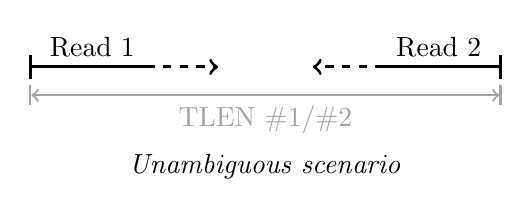
\begin{tikzpicture}[
    thick, xscale=2, yscale=1.8,
    read/.style={line width=0.4mm},
]
\draw[|-, read] (0,0)   -- (0.8,0)  node[midway, above] {Read 1};
\draw[->, read, dashed] (0.85,0) -- (1.2,0);
\draw[|-, read] (3,0) -- (2.2,0) node[midway, above] {Read 2};
\draw[->, read, dashed] (2.25,0) -- (1.8,0);
\draw[|<->|,gray!120]     (0,-.2) -- +(3,0) node[midway, below] {TLEN \#1/\#2};
\node at (1.5,-0.7) {\textit{Unambiguous scenario}};
\end{tikzpicture}
\hspace{3cm}% No space means side by side
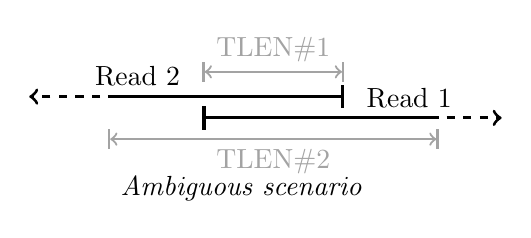
\begin{tikzpicture}[
    thick, xscale=1,yscale=0.9,
    read/.style={line width=0.4mm},
]
\draw[|-, read]         (2.2,0)   -- (5.2,0)    node[very near end, above] {Read 1};
\draw[->, read, dashed] (5.3,0)   -- (6,0);
\draw[-|, read]         (1,.3)    -- (4,.3)     node[very near start , above] {Read 2};
\draw[->, read, dashed] (0.9,.3)  -- (0,.3);
\draw[|<->|,gray!120]   (1,-0.3)  -- (5.2,-0.3) node[midway, below] {TLEN\#2};
\draw[|<->|,gray!120]   (2.2,0.65)-- (4,0.65)    node[midway, above] {TLEN\#1};
\node at (2.7,-1) {\textit{Ambiguous scenario}};
\end{tikzpicture}
\end{center}
}

\item {\sf SEQ}: segment SEQuence. This field can be a `*' when the
  sequence is not stored. If not a `*', the length of the sequence must
  equal the sum of lengths of {\tt M/I/S/=/X} operations in {\sf CIGAR}.
  An `=' denotes the base is identical to the reference base. No
  assumptions can be made on the letter cases.
\item {\sf QUAL}: ASCII of base QUALity plus 33 (same as the quality
  string in the Sanger FASTQ format). A base quality is the phred-scaled
  base error probability which equals $-10\log_{10}\Pr\{\mbox{base is
    wrong}\}$. This field can be a `*' when quality is not stored. If
  not a `*', {\sf SEQ} must not be a `*' and the length of the quality string
  ought to equal the length of {\sf SEQ}.
\end{enumerate}

\subsection{The alignment section: optional fields}\label{sec:alnaux}
All optional fields follow the {\tt TAG:TYPE:VALUE} format
where {\tt TAG} is a two-character string that matches {\tt /[A-Za-z][A-Za-z0-9]/}.
Each {\tt TAG} can only appear once in one alignment line. A {\tt TAG}
containing lowercase letters are reserved for end users.
In an optional field, {\tt TYPE} is a single case-sensitive letter which
defines the format of {\tt VALUE}:
\begin{center}\small
\begin{tabular}{cll}
\hline
{\bf Type} & {\bf Regexp matching {\tt VALUE}} & {\bf Description} \\
\hline
A & {\tt [!-\char126]} & Printable character \\
i & {\tt [-+]?[0-9]+} & Signed integer\footnotemark\\
f & {\tt [-+]?[0-9]*\char92.?[0-9]+([eE][-+]?[0-9]+)?} & Single-precision floating number \\
Z & {\tt [\,\,\,!-\char126]*} & Printable string, including space\\
H & {\tt ([0-9A-F][0-9A-F])*} & Byte array in the Hex format\footnotemark\\
B & {\tt [cCsSiIf](,[-+]?[0-9]*\char92.?[0-9]+([eE][-+]?[0-9]+)?)*} & Integer or numeric array\\
\hline
\end{tabular}
\addtocounter{footnote}{-1}
\footnotetext{The number of digits in an integer optional field is not
explicitly limited in SAM.  However, BAM can represent values in the
range~$[-2^{31},2^{32})$, so in practice this is the realistic range
of values for SAM's `{\tt i}' as well.}
\stepcounter{footnote}
\footnotetext{For example, the six-character Hex string `{\tt 1AE301}' represents the byte array $[{\tt 0x1a},{\tt 0xe3},{\tt 0x1}]$.}
\end{center}
For an integer or numeric array (type `{\tt B}'), the first letter indicates the type of numbers
in the following comma separated array. The letter can be one of `{\tt cCsSiIf}', corresponding to
{\tt int8\_t} (signed 8-bit integer), {\tt uint8\_t} (unsigned 8-bit integer), {\tt int16\_t}, {\tt uint16\_t}, {\tt int32\_t}, {\tt uint32\_t}
and {\tt float}, respectively.\footnotemark\@ During import/export, the element type
may be changed if the new type is also compatible with the array.
\footnotetext{Explicit typing eases format parsing and helps to reduce the file size when SAM is converted to BAM.}

Predefined tags are described in the separate {\sl Sequence Alignment/Map
Optional Fields Specification}.\footnote{See
\href{http://samtools.github.io/hts-specs/SAMtags.pdf}{\tt SAMtags.pdf}
at \url{https://github.com/samtools/hts-specs}.}
See that document for details of existing standard tag fields and conventions
around creating new tags that may be of general interest.
Tags starting with `{\tt X}', `{\tt Y}' or `{\tt Z}' and tags containing
lowercase letters in either position are reserved for local use and will
not be formally defined in any future version of these specifications.

\pagebreak

\section{Recommended Practice for the SAM Format}
\label{sec:recommended-practice}
This section describes the best practice for representing data in the
SAM format. They are not required in general, but may be required by a
specific software package for it to function properly.

\begin{enumerate}
\item The header section
  \begin{enumerate}[label=\arabic*]
  \item The {\tt @HD} line should be present, with either the {\tt SO} tag
    or the {\tt GO} tag (but not both) specified.
  \item The {\tt @SQ} lines should be present if reads have been mapped.
  \item When a {\tt RG} tag appears anywhere in the alignment section,
    there should be a single corresponding {\tt @RG} line with matching
    {\tt ID} tag in the header.
  \item When a {\tt PG} tag appears anywhere in the alignment section,
    there should be a single corresponding {\tt @PG} line with matching
    {\tt ID} tag in the header.
  \end{enumerate}
\item Adjacent CIGAR operations should be different.
\item No alignments should be assigned mapping quality 255.
\item Unmapped reads
  \begin{enumerate}[label=\arabic*]
  \item For a unmapped paired-end or mate-pair read whose mate is
    mapped, the unmapped read should have {\sf RNAME} and {\sf POS}
    identical to its mate.
  \item If all segments in a template are unmapped, their {\sf RNAME}
    should be set as `*' and {\sf POS} as 0.
  \item If {\sf POS} plus the sum of lengths of {\tt M/=/X/D/N}
    operations in {\sf CIGAR} exceeds the length specified in the {\tt
      LN} field of the {\tt @SQ} header line (if exists) with an SN
    equal to {\sf RNAME}, the alignment should be unmapped, unless the
    reference sequence is circular (see below).
  \item Unmapped reads should be stored in the orientation in which they came
    off the sequencing machine and have their {\sf reverse} flag bit~(0x10)
    correspondingly unset.
  \end{enumerate}
\item Multiple mapping
  \begin{enumerate}[label=\arabic*]
  \item When one segment is present in multiple lines to represent a multiple
	mapping of the segment, only one of these records should have the secondary
	alignment flag bit (0x100) unset. {\sf RNEXT} and {\sf PNEXT} point to the
	primary line of the next read in the template.
  \item {\sf SEQ} and {\sf QUAL} of secondary alignments should be set
    to `*' to reduce the file size.
  \end{enumerate}
%\item There should be no overlap between segments of a read\footnote{Few/no
%  existing aligners follow this practice.}.
\item Optional tags:
  \begin{enumerate}[label=\arabic*]
  \item If the template has more than 2 segments, the {\tt TC} tag
    should be present.
  \item The {\tt NM} tag should be present.
  \end{enumerate}

\item Circular reference sequences

Mappings that cross the coordinate `join' in circular reference sequences (i.e., those whose {\tt @SQ} headers specify {\tt TP:circular}) may be represented as follows:
  \begin{enumerate}[label=\arabic*]
  \item (Preferred)
As usual {\sf POS} should be between 1 and the {\tt @SQ} header's {\tt LN} value, but {\sf POS} plus the sum of the lengths of {\tt M/=/X/D/N} {\sf CIGAR} operations may exceed {\tt LN}.
Coordinates greater than~{\tt LN} are interpreted by subtracting {\tt LN} so that bases at $\texttt{LN}+1, \texttt{LN}+2, \texttt{LN}+3, \ldots$ are considered to be mapped at positions $1,2,3,\ldots$; thus each (1-based) position $p$ is interpreted as $((p-1)\bmod\texttt{LN})+1$.%
\footnote{The impact of this representation on indexing and random access is yet to be explored by implementations.}

  \item
Alternatively, such alignments may be split across several records: one record representing the initial portion of the segment ending at~{\tt LN}, one representing the final portion starting from~1, and any other records representing additional portions in between spanning the entire reference sequence.
One record (chosen arbitrarily) is considered primary and the remainder have their {\sf supplementary} flag bit (0x800) set.
  \end{enumerate}

\item Annotation dummy reads:
  These have {\sf SEQ} set to {\tt *}, {\sf FLAG} bits 0x100 and 0x200
  set (secondary and filtered), and a {\tt CT} tag.
  \begin{enumerate}[label=\arabic*]
%Repeating what is in the tag's footnote:
%  \item If the {\tt CT} tag's \emph{strand} is {\tt -}, FLAG bit 0x10
%  (reverse complemented) should be set, and otherwise not set.
  \item If you wish to store free text in a {\tt CT} tag, use the
  \emph{key} value {\tt Note} (uppercase N) to match GFF3.
  \item Multi-segment annotation (e.g., a gene with introns) should be
  described with multiple lines in SAM (like a multi-segment read).
  Where there is a clear biological direction (e.g., a gene), the first
  segment ({\sf FLAG} bit 0x40) is used for the first section (e.g., the
  $5'$ end of the gene). Thus a GenBank entry location like
  {\tt complement(join(85052..85354, 85441..85621, 86097..86284))}
  would have three lines in SAM with a common {\sf QNAME}: %And three lines in GFF3 too.
    \begin{center}\begin{tabular}{llrcl}
  & \multicolumn{1}{c}{\sf FLAG} & \multicolumn{1}{c}{\sf POS} & \sf CIGAR & \multicolumn{1}{c}{Optional fields} \\
The $5'$ fragment & 883 (0x373) & 86097 & \tt 188M & \tt FI:i:1\quad TC:i:3 \\
Middle fragment   & 819 (0x333) & 85441 & \tt 181M & \tt FI:i:2\quad TC:i:3 \\
The $3'$ fragment & 947 (0x3B3) & 85052 & \tt 303M & \tt FI:i:3\quad TC:i:3
    \end{tabular}\end{center}
  \item If converting GFF3 to SAM, store any \emph{key}, \emph{values}
  from column 9 in the {\tt CT} tag, except for the unique ID which
  is used for the QNAME. GFF3 columns 1 (seqid), 4 (start) and 5 (end)
  are encoded using SAM columns RNAME, POS and CIGAR to hold the length.
  GFF3 columns 3 (type) and 7 (strand) are stored explicitly in the
  {\tt CT} tag. Remaining GFF3 columns 2 (source), 6 (score), and
  8 (phase) are stored in the {\tt CT} tag using \emph{key} values
  {\tt FSource}, {\tt FScore} and {\tt FPhase} (uppercase keys are
  restricted in GFF3, so these names avoid clashes). Split location
  features are described with multiple lines in GFF3, and similarly
  become multi-segment dummy reads in SAM, with the {\sf RNEXT} and
  {\sf PNEXT} columns filled in appropriately. In the absence of a
  convention in SAM/BAM for reads wrapping the origin of a circular
  genome, any GFF3 feature line wrapping the origin must be split into
  two segments in SAM.
  \end{enumerate}
\end{enumerate}

\section{Guide for Describing Assembly Sequences in SAM}

\subsection{Unpadded versus padded representation}

To describe alignments, we can regard the reference sequence with no respect to
other alignments against it.  Such a reference sequence is called an
\emph{unpadded reference}. A position on an unpadded reference, referred to
as an \emph{unpadded position}, is not affected by any alignments. When we use
unpadded references and positions to describe alignments, we say we are using
the \emph{unpadded representation}.

Alternatively, to describe the same alignments, we can modify the reference
sequence to contain pads that make room for sequences inserted relative to the
reference. A pad is effectively a gap and conventionally represented by an
asterisk `*'.  A reference sequence containing pads is called a \emph{padded
reference}. A position which counts the *'s is referred to as a \emph{padded
position}. A padded reference sequence may be affected by the query alignments
and because of gap insertions is typically longer than the unpadded reference.
The padded position of one query alignment may be affected by other query
alignments.

Unpadded and padded are different representations of the same alignments. They
are convertible to each other with no loss of any information. The unpadded
representation is more common due to the convenience of a fixed coordinate system,
while the padded representation has the advantage that alignments can be simply
described by the start and end coordinates without using complex CIGAR strings.
SAM traditionally uses the padded representation for {\it de novo} assembly.
The ACE assembly format uses the padded representation exclusively.

\subsection{Padded SAM}\label{sec:padded-sam}

The SAM format is typically used to describe alignments against an unpadded
reference sequence, but it is also able to describe alignments against a padded
reference. In the latter case, we say we are using a \emph{padded SAM}. A padded
SAM is a valid SAM, but with the difference that the reference and positions in
use are padded. There may be more than one way to describe the padded
representation.
We recommend the following; see also the discussion in Cock {\it et al.}%
\footnote{Peter J. A. Cock, James K. Bonfield, Bastien Chevreux, and Heng Li,
{\bf SAM/BAM format v1.5 extensions for \emph{de novo} assemblies},
{\sl bioRxiv 020024};
\href{http://dx.doi.org/10.1101/020024}{doi:10.1101/020024}.}

In a padded SAM, alignments and coordinates are described with respect to the
padded reference sequence. Unlike traditional padded representations like
the ACE file format where pads/gaps are recorded in reads using *'s, we do
not write *'s in the {\sf SEQ} field of the SAM format.\footnote{Writing
pads/gaps as *'s in the {\sf SEQ} field might have been more convenient, but
this caused concerns for backward compatibility.} Instead, we describe pads
in the query sequences as deletions from the padded reference using the
{\sf CIGAR} `{\tt D}' operation. In a padded SAM, the insertion and padding
CIGAR operations (`{\tt I}' and `{\tt P}') are not used because the padded
reference already considers all the insertions.

The following shows the padded SAM for the example alignment in Section~\ref{sec:example}.
Notably, the length of {\tt ref} is 47 instead of 45. {\sf POS} of the last
three alignments are all shifted by 2. {\sf CIGAR} of alignments bridging the
2bp insertion are also changed.

\begin{framed}\small
\begin{verbatim}
@HD VN:1.6 SO:coordinate
@SQ SN:ref LN:47
ref   516 ref  1  0 14M2D31M   *  0   0 AGCATGTTAGATAAGATAGCTGTGCTAGTAGGCAGTCAGCGCCAT *
r001   99 ref  7 30 14M1D3M    = 39  41 TTAGATAAAGGATACTG *
*     768 ref  8 30 1M         *  0   0 *                 * CT:Z:.;Warning;Note=Ref wrong?
r002    0 ref  9 30 3S6M1D5M   *  0   0 AAAAGATAAGGATA    * PT:Z:1;4;+;homopolymer
r003    0 ref  9 30 5H6M       *  0   0 AGCTAA            * NM:i:1
r004    0 ref 18 30 6M14N5M    *  0   0 ATAGCTTCAGC       *
r003 2064 ref 31 30 6H5M       *  0   0 TAGGC             * NM:i:0
r001  147 ref 39 30 9M         =  7 -41 CAGCGGCAT         * NM:i:1
\end{verbatim}
\end{framed}

Here we also exemplify the recommended practice for storing the reference
sequence and the reference annotations in SAM when necessary. For a reference
sequence in SAM, {\sf QNAME} should be identical to {\sf RNAME}, {\sf POS} set
to 1 and {\sf FLAG} to 516 (filtered and unmapped); for an annotation, {\sf
FLAG} should be set to 768 (filtered and secondary) with no restriction to {\sf
QNAME}.
Dummy reads for annotation would typically have a {\tt CT} tag to hold the annotation information; see the discussion of dummy reads in Section~\ref{sec:recommended-practice}.
See also the separate {\sl Optional Fields Specification} for full details of the {\tt CT} and {\tt PT} annotation tags.%
\footnote{See \emph{Annotation and Padding} in \href{http://samtools.github.io/hts-specs/SAMtags.pdf}{\tt SAMtags.pdf}.}

\pagebreak

\section{The BAM Format Specification}

\subsection{The BGZF compression format}

BGZF is block compression implemented on top of the standard gzip file
format.\footnote{L.~Peter Deutsch, {\bf GZIP file format specification
version~4.3}, \href{http://tools.ietf.org/html/rfc1952}{\sl RFC 1952}.}
The goal of BGZF is to provide good compression while allowing
efficient random access to the BAM file for indexed queries. The BGZF
format is `gunzip compatible', in the sense that a compliant gunzip
utility can decompress a BGZF compressed file.\footnote{It is worth noting that there is a known bug in the Java {\sf
  GZIPInputStream} class that concatenated gzip archives cannot be
successfully decompressed by this class. BGZF files can be created and
manipulated using the built-in Java {\sf util.zip} package, but naive
use of {\sf GZIPInputStream} on a BGZF file will not work due to this
bug.}

A BGZF file is a series of concatenated BGZF blocks, each no larger
than~64Kb before or after compression. Each BGZF block
is itself a spec-compliant gzip archive which contains an ``extra field''
in the format described in RFC1952. The gzip file format allows the
inclusion of application-specific extra fields and these are ignored by
compliant decompression implementation. The gzip specification also
allows gzip files to be concatenated. The result of decompressing
concatenated gzip files is the concatenation of the uncompressed data.

Each BGZF block contains a standard gzip file header with the following
standard-compliant extensions:

\begin{enumerate}
\item The {\sf F.EXTRA} bit in the header is set to indicate that extra
  fields are present.
\item The extra field used by BGZF uses the two subfield ID values 66 and 67 (ascii `BC').
\item The length of the BGZF extra field payload (field {\sf LEN} in the
  gzip specification) is 2 (two bytes of payload).
\item The payload of the BGZF extra field is a 16-bit unsigned integer
  in little endian format. This integer gives the size of the containing
  BGZF block minus one.
\end{enumerate}

On disk, a complete BGZF file is a series of blocks as shown in the following
table.  (All integers are little endian as is required by RFC1952.)
\begin{table}[ht]
\centering
{\small
\begin{tabular}{|l|l|l|l|l|r|}
  \cline{1-6}
  \multicolumn{3}{|c|}{\bf Field} & \multicolumn{1}{c|}{\bf Description} & \multicolumn{1}{c|}{\bf Type} & \multicolumn{1}{c|}{\bf Value} \\\cline{1-6}
  \multicolumn{6}{|c|}{\textcolor{gray}{\it List of compression blocks (until the end of the file)}} \\\cline{2-6}
  & \multicolumn{2}{l|}{\sf ID1} & gzip IDentifier1 & {\tt uint8\_t} & 31 \\\cline{2-6}
  & \multicolumn{2}{l|}{\sf ID2} & gzip IDentifier2 & {\tt uint8\_t} & 139 \\\cline{2-6}
  & \multicolumn{2}{l|}{\sf CM} & gzip Compression Method & {\tt uint8\_t} & 8 \\\cline{2-6}
  & \multicolumn{2}{l|}{\sf FLG} & gzip FLaGs & {\tt uint8\_t} & 4 \\\cline{2-6}
  & \multicolumn{2}{l|}{\sf MTIME} & gzip Modification TIME & {\tt uint32\_t} & \\\cline{2-6}
  & \multicolumn{2}{l|}{\sf XFL} & gzip eXtra FLags & {\tt uint8\_t} & \\\cline{2-6}
  & \multicolumn{2}{l|}{\sf OS} & gzip Operating System & {\tt uint8\_t} & \\\cline{2-6}
  & \multicolumn{2}{l|}{\sf XLEN} & gzip eXtra LENgth & {\tt uint16\_t} & \\\cline{2-6}
  & \multicolumn{5}{c|}{\textcolor{gray}{\it Extra subfield(s) (total size=XLEN)}} \\\cline{3-6}
  & & \multicolumn{4}{c|}{\textcolor{gray}{\it Additional RFC1952 extra subfields if present}} \\\cline{3-6}
  & & {\sf SI1} & Subfield Identifier1 & {\tt uint8\_t} & 66 \\\cline{3-6}
  & & {\sf SI2} & Subfield Identifier2 & {\tt uint8\_t} & 67 \\\cline{3-6}
  & & {\sf SLEN} & Subfield LENgth & {\tt uint16\_t} & 2 \\\cline{3-6}
  & & {\sf BSIZE} & total Block SIZE minus 1 & {\tt uint16\_t} & \\\cline{3-6}
  & & \multicolumn{4}{c|}{\textcolor{gray}{\it Additional RFC1952 extra subfields if present}} \\\cline{2-6}
  & \multicolumn{2}{l|}{\sf CDATA} & Compressed DATA by {\sf zlib::deflate()} & {\tt uint8\_t[{\sf BSIZE-XLEN-19}]} & \\\cline{2-6}
  & \multicolumn{2}{l|}{\sf CRC32} & CRC-32 & {\tt uint32\_t} & \\\cline{2-6}
  & \multicolumn{2}{l|}{\sf ISIZE} & Input SIZE (length of uncompressed data) & {\tt uint32\_t} & \\
  \cline{1-6}
\end{tabular}}
\end{table}

The random access method to be described next limits the uncompressed
contents of each BGZF block to a maximum of $2^{16}$~bytes of data.
Thus while {\sf ISIZE} is stored as a {\tt uint32\_t} as per the gzip format,
in BGZF it is limited to the range~$[0,65536]$.
{\sf BSIZE} can represent BGZF block sizes in the range~$[1,65536]$, though
typically {\sf BSIZE} will be rather less than~{\sf ISIZE} due to compression.

\subsubsection{Random access}

BGZF files support random access through the BAM file index. To achieve
this, the BAM file index uses \emph{virtual file offsets} into the BGZF
file. Each virtual file offset is an unsigned 64-bit integer, defined as: {\tt
  coffset\char60\char60 16\char124uoffset}, where {\tt coffset} is an
unsigned byte offset into the BGZF file to the beginning of a BGZF
block, and {\tt uoffset} is an unsigned byte offset into the
uncompressed data stream represented by that BGZF block. Virtual file
offsets can be compared, but subtraction between virtual file offsets
and addition between a virtual offset and an integer are both
disallowed.

\subsubsection{End-of-file marker}

An end-of-file (EOF) trailer or marker block should be written at the end
of BGZF files, so that unintended file truncation can be easily detected.
The EOF marker block is a particular empty\footnotemark\ BGZF block
encoded with the default {\sf zlib} compression level settings,
and consists of the following 28~hexadecimal bytes:
\begin{center}
\texttt{1f 8b 08 04 00 00 00 00 00 ff 06 00 42 43 02 00 1b 00 03 00 00 00 00 00 00 00 00 00}
\end{center}

\footnotetext{Empty in the sense of having been formed by compressing
a data block of length zero.}

\noindent
The presence of this EOF marker at the end of a BGZF file indicates that the
immediately following physical EOF is the end of the file as intended by the
program that wrote it.
Empty BGZF blocks are not otherwise special; in particular, the presence of
an EOF marker block does not by itself signal end of file.\footnotemark

\footnotetext{An implementation that supports reopening a BAM file in append
mode could produce a file by writing headers and alignment records to it,
closing it (adding an EOF marker); then reopening it for append, writing
more alignment records, and closing it (adding an EOF marker).
The resulting BAM file would contain an embedded insignificant EOF~marker
block that should be effectively ignored when it is read.}

The absence of this final EOF marker should trigger a warning or error
soon after opening a BGZF file where random access is available.\footnotemark\
When reading a BGZF file in sequential streaming fashion, ideally this
EOF check should be performed when the end of the stream is reached.
Checking that the final BGZF block in the file decompresses to empty
or checking that the last 28 bytes of the file are exactly the bytes
above are both sufficient tests; each is likely more convenient in
different circumstances.

\footnotetext{It is useful to produce a diagnostic at the beginning of
reading a file, so that interactive users can abort lengthy analysis of
potentially-corrupted files.  Of course, this is only possible if the
stream in question supports random access.}

\pagebreak

\subsection{The BAM format}
BAM is compressed in the BGZF format. All multi-byte numbers in BAM are
little-endian, regardless of the machine endianness. The format is
formally described in the following table where values in brackets are
the default when the corresponding information is not available; an
underlined word in uppercase denotes a field in the SAM format.

\begin{table}[ht]
\centering
{\small
\begin{tabular}{|l|l|l|p{8.15cm}|l|r|}
  \cline{1-6}
  \multicolumn{3}{|c|}{\bf Field} & \multicolumn{1}{c|}{\bf Description} & \multicolumn{1}{c|}{\bf Type} & \multicolumn{1}{c|}{\bf Value} \\\cline{1-6}
  \multicolumn{3}{|l|}{\sf magic} & BAM magic string & {\tt char[4]} & {\tt BAM\char92 1}\\\cline{1-6}
  \multicolumn{3}{|l|}{\sf l\_text} & Length of the header text, including any {\tt NUL} padding & {\tt uint32\_t} & $< 2^{31}$ \\\cline{1-6}
  \multicolumn{3}{|l|}{\sf text} & Plain header text in SAM; not necessarily {\tt NUL}-terminated & {\tt char[{\sf l\_text}]} & \\\cline{1-6}
  % Pedantically this should be <= but we restrict |refs| by one so n_ref fits in a signed 32-bit int.
  \multicolumn{3}{|l|}{\sf n\_ref} & \# reference sequences & {\tt uint32\_t} & $< 2^{31}$ \\\cline{1-6}
  \multicolumn{6}{|c|}{\textcolor{gray}{\it List of reference information (n=n\_ref)}} \\\cline{2-6}
  & \multicolumn{2}{l|}{\sf l\_name} & Length of the reference name plus 1 (including {\tt NUL}) & {\tt uint32\_t} & \memlimited \\\cline{2-6}
  & \multicolumn{2}{l|}{\sf name} & Reference sequence name; {\tt NUL}-terminated & {\tt char[{\sf l\_name}]} & \\\cline{2-6}
  & \multicolumn{2}{l|}{\sf l\_ref} & Length of the reference sequence & {\tt uint32\_t} & $< 2^{31}$ \\\cline{1-6}
  \multicolumn{6}{|c|}{\textcolor{gray}{\it List of alignments (until the end of the file)}} \\\cline{2-6}
  & \multicolumn{2}{l|}{\sf block\_size} & Total length of the alignment record, excluding this field & {\tt uint32\_t} & \memlimited \\\cline{2-6}
  & \multicolumn{2}{l|}{\sf refID} & Reference sequence ID, $-1\leq{\sf refID}<{\sf n\_ref}$; -1 for a read without a mapping position & {\tt int32\_t} & [-1] \\\cline{2-6}
  & \multicolumn{2}{l|}{\sf pos} & 0-based leftmost coordinate ($=\underline{\sf POS}-1$)& {\tt int32\_t} & [-1]\\\cline{2-6}
  & \multicolumn{2}{l|}{\sf l\_read\_name} & Length of {\sf read\_name} below ($={\sf length}(\underline{\sf QNAME})+1$) & {\tt uint8\_t} & \\\cline{2-6}
  & \multicolumn{2}{l|}{\sf mapq} & Mapping quality (=\underline{\sf MAPQ}) & {\tt uint8\_t} & \\\cline{2-6}
  & \multicolumn{2}{l|}{\sf bin} & BAI index bin, see Section~\ref{sec:bin-field}  & {\tt uint16\_t} & \\\cline{2-6}
  & \multicolumn{2}{l|}{\sf n\_cigar\_op} & Number of operations in \underline{\sf CIGAR}, see Section~\ref{sec:ncigar} & {\tt uint16\_t} & \\\cline{2-6}
  & \multicolumn{2}{l|}{\sf flag} & Bitwise flags (= \underline{\sf FLAG})\footnotemark\ & {\tt uint16\_t} & \\\cline{2-6}
  & \multicolumn{2}{l|}{\sf l\_seq} & Length of \underline{\sf SEQ} & {\tt uint32\_t} & \memlimited \\\cline{2-6}
  & \multicolumn{2}{l|}{\sf next\_refID} & Ref-ID of the next segment ($-1\le{\sf next\_refID}<{\sf n\_ref}$) & {\tt int32\_t} & [-1] \\\cline{2-6}
  & \multicolumn{2}{l|}{\sf next\_pos} & 0-based leftmost pos of the next segment ($=\underline{\sf PNEXT}-1$) & {\tt int32\_t} & [-1] \\\cline{2-6}
  & \multicolumn{2}{l|}{\sf tlen} & Template length ($=\underline{\sf TLEN}$) & {\tt int32\_t} & [0] \\\cline{2-6}
  & \multicolumn{2}{l|}{\sf read\_name} & Read name, {\tt NUL}-terminated (\underline{\sf QNAME} with trailing `{\tt\verb"\0"}')\footnotemark & {\tt char[{\sf l\_read\_name}]} & \\\cline{2-6}
  & \multicolumn{2}{l|}{\sf cigar} & CIGAR: {\tt {\sf op\_len}\char60\char60 4\char124{\sf op}}. `{\tt MIDNSHP\char61X}'$\to$`012345678' & {\tt uint32\_t[{\sf n\_cigar\_op}]} & \\\cline{2-6}
  & \multicolumn{2}{l|}{\sf seq} & 4-bit encoded read: `{\tt =ACMGRSVTWYHKDBN}'$\to[0,15]$. See Section~\ref{sec:seq} & {\tt uint8\_t[({\sf l\_seq}+1)/2]} & \\\cline{2-6}
  & \multicolumn{2}{l|}{\sf qual} & Phred-scaled base qualities. See Section~\ref{sec:seq} & {\tt char[{\sf l\_seq}]} & \\\cline{2-6}
  & \multicolumn{5}{c|}{\textcolor{gray}{\it List of auxiliary data (until the end of the alignment block)}} \\\cline{3-6}
  & & {\sf tag} & Two-character tag & {\tt char[2]} & \\\cline{3-6}
  & & {\sf val\_type} & Value type: {\tt AcCsSiIfZHB}, see Section~\ref{sec:aux-type-codes} & {\tt char} & \\\cline{3-6}
  & & {\sf value} & Tag value & (by {\sf val\_type}) &\\
  \cline{1-6}
\end{tabular}}
\end{table}
\addtocounter{footnote}{-1}
\footnotetext{As noted in Section~\ref{sec:alnrecord}, reserved {\sf FLAG} bits
should be written as zero and ignored on reading by current software.}
\stepcounter{footnote}
\footnotetext{For backward compatibility, an absent {\sf QNAME} (represented as `{\tt *}' in SAM) is stored as a C string {\tt "*\char92 0"}.}

\noindent
Most length and count fields described as {\tt uint32\_t} have additional constraints on their range:
$\mbox{\sf l\_text} < 2^{31}$ due to implementation limits;
$\mbox{\sf n\_ref} < 2^{31}$ because {\sf refID} and {\sf next\_refID} are signed;
$\mbox{\sf l\_ref} < 2^{31}$ because {\sf tlen} is signed;
those marked ``\textit{limited}'' are limited by available memory and the practical size of the data represented well before they are limited by, e.g., Java's signed 32-bit integer maximum array size.

\subsubsection{BIN field calculation}\label{sec:bin-field}
{\sf BIN} is calculated using the {\sf reg2bin()} function in
Section~\ref{sec:code}.
For mapped reads this uses {\sf POS-1} (i.e.,~0-based left position) and the
alignment end point using the alignment length from the {\sf CIGAR} string.
For unmapped reads (e.g.,~paired end reads where only one part is mapped, see
Section~\ref{sec:recommended-practice}) the alignment is treated as
being length one.
Note unmapped reads with {\sf POS} $0$ (which becomes $-1$ in BAM) therefore
use {\sf reg2bin(-1, 0)} which is $4680$.

\subsubsection{N\_CIGAR\_OP field}\label{sec:ncigar}
With 16 bits, {\sf n\_cigar\_op} can keep at most 65535 CIGAR
operations in BAM files. For an alignment with more CIGAR operations, BAM
stores the real {\sf CIGAR}, encoded the same way as the {\sf cigar} field in
BAM, in the {\tt CG} optional tag of type `{\tt B,I}', and sets {\sf CIGAR} to
`\textit{k}{\tt S}\textit{m}{\tt N}' as a placeholder, where `\textit{k}' equals {\sf l\_seq}, `\textit{m}'
is the reference sequence length in the alignment, and `{\tt S}' and `{\tt N}'
are the soft-clipping and reference-clip CIGAR operators, respectively---i.e.,
in the binary form, {\sf n\_cigar\_op}=2 and {\sf cigar}={\tt [\textit{k}\char60\char60
4\char124{4},\textit{m}\char60\char60 4\char124{3}]}. If tag {\tt CG} is present and
the first CIGAR operation clips the entire read, a BAM parsing library is
expected to update {\sf n\_cigar\_op} and {\sf cigar} with the real CIGAR
stored in the {\tt CG} tag and remove the now-redundant {\tt CG} tag.

\subsubsection{SEQ and QUAL encoding}\label{sec:seq}
Sequence is encoded in 4-bit values, with adjacent bases packed into the same byte starting with the highest 4 bits first.
When {\sf l\_seq} is odd the bottom 4 bits of the last byte are undefined, but we recommend writing these as zero.
The case-insensitive base codes `{\tt =ACMGRSVTWYHKDBN}' are mapped to $[0,15]$ respectively with all other characters mapping to `{\tt N}' (value 15).

Omitted sequence, represented in SAM as `{\tt *}', is represented by {\sf l\_seq} being 0 and {\sf seq} and {\sf qual} zero-length.

Base qualities are stored as bytes in the range $[0,93]$, without any +33 conversion to printable ASCII.
When base qualities are omitted but the sequence is not, {\sf qual} is filled with {\tt 0xFF} bytes (to length {\sf l\_seq}).

\subsubsection{Auxiliary data encoding}\label{sec:aux-type-codes}
Optional alignment fields are stored immediately after each other immediately
following the {\sf qual} field, and are included in {\sf block\_size}.
Each field is represented as a two-character tag followed by a single type
character and then its value, whose length is determined by the field's type.

\newcommand*{\tagfield}[2]{\firstbytebox{2}{\em tag}\bytebox{1}{\tt #1}#2}

Single character `{\tt A}' fields have a total length of 4~bytes,
with the value represented as a single byte:
\begin{center}\small\byteboxsetup
\tagfield{A}{\bytebox{1}{char}}
\end{center}

While all single (i.e., non-array) integer types are stored in SAM as `{\tt i}',
in BAM any of `{\tt cCsSiI}' may be used together with the correspondingly-sized
binary integer value, chosen according to the field value's magnitude.%
\footnote{The signedness and size used for each integer value is an
implementation choice, but is typically the smallest that suffices.}
Similarly floating point `{\tt f}' fields are represented as IEEE 754-2008
binary32 values.
Thus BAM numeric fields have a total length of~4, 5, or~7~bytes:
\begin{center}\small\byteboxsetup\begin{tabular}{l@{\hspace{1in}}l}
\tagfield{c}{\bytebox{1}{i8}} \quad (i.e., {\tt int8\_t})
    & \tagfield{i}{\bytebox{4}{int32\_t}} \\
\tagfield{C}{\bytebox{1}{u8}} \quad (i.e., {\tt uint8\_t})
    & \tagfield{I}{\bytebox{4}{uint32\_t}} \\
\tagfield{s}{\bytebox{2}{int16\_t}}
    & \tagfield{f}{\bytebox{4}{float}} \\
\tagfield{S}{\bytebox{2}{uint16\_t}}
    &
\end{tabular}\end{center}

\newcommand*{\byteboxvector}[2]{\bytebox{#1}{#2}\bytebox{#1}{#2}\makebox[1.5\bytewidth][c]{$\cdots$}\firstbytebox{#1}{#2}}

String fields and hex-formatted byte arrays are represented as
{\tt NUL}-terminated text strings:%
\footnote{The BAM representation of `{\tt H}' field values as textual
hexadecimal digits rather than binary data is for historical reasons.
Modern applications may prefer to use `{\tt B,C}' array fields rather
than `{\tt H}' fields.}
\begin{center}\small\byteboxsetup\begin{tabular}{l}
\tagfield{Z}{\byteboxvector{1}{char}\bytebox{1}{\tt NUL}} \\
\tagfield{H}{\byteboxvector{2}{hex hex}\bytebox{1}{\tt NUL}}
\end{tabular}\end{center}

\newcommand*{\arraytagfield}[3]{\tagfield{B}{\bytebox{1}{\tt #1}\bytebox{4}{\em count}\byteboxvector{#2}{#3}}}

\begin{samepage}
The representation of a `{\tt B}' array field starts with a sub-type character
similar to the numeric field types above and a \emph{count} ({\tt uint32\_t}, but
limited by memory and {\sf block\_size}) giving the number of elements in the array.
The array elements follow, encoded as binary integers or IEEE floats sized
according to the sub-type:
\begin{center}\small\byteboxsetup\begin{tabular}{l}
\arraytagfield{c}{1}{i8} \quad (i.e., {\tt int8\_t} elements) \\
\arraytagfield{C}{1}{u8} \quad (i.e., {\tt uint8\_t} elements) \\
\arraytagfield{s}{2}{int16\_t} \\
\arraytagfield{S}{2}{uint16\_t} \\
\arraytagfield{i}{4}{int32\_t} \\
\arraytagfield{I}{4}{uint32\_t} \\
\arraytagfield{f}{4}{float}
\end{tabular}\end{center}
\end{samepage}

\pagebreak

\section{Indexing BAM}
Indexing aims to achieve fast retrieval of alignments overlapping a
specified region without going through the whole alignments. BAM must be
sorted by the reference ID and then the leftmost coordinate before
indexing.

This section describes the binning scheme underlying coordinate-sorted
BAM indices and its implementation in the long-established BAI format.
The CSI format documented elsewhere uses a similar binning scheme and
can also be used to index BAM.\footnotemark

\footnotetext{See \href{http://samtools.github.io/hts-specs/CSIv1.pdf}
{\tt CSIv1.pdf} at \url{https://github.com/samtools/hts-specs}.
This is a separate specification because CSI is also used to index other
coordinate-sorted file formats in addition to BAM.}

\subsection{Algorithm}
\subsubsection{Basic binning index}
The UCSC binning scheme was suggested by Richard Durbin and Lincoln Stein
and is explained in Kent {\it et al.}\footnotemark\ In this scheme, each bin
represents a contiguous genomic region which is either fully contained
in or non-overlapping with another bin; each alignment is associated
with a bin which represents the smallest region containing the entire
alignment. The binning scheme is essentially a representation of
R-tree. A distinct bin uniquely corresponds to a distinct internal node
in a R-tree. Bin A is a child of Bin B if the region represented by A is
contained in B.

\footnotetext{W.~James Kent {\it et al.},
{\bf The Human Genome Browser at UCSC}, {\sl Genome Res.}~2002~12: 996--1006;
\href{http://dx.doi.org/doi:10.1101/gr.229102}{doi:10.1101/\linebreak[1]gr.229102};
{\sc pmid:}12045153.  See in particular {\sl The Database}, p1003.}

To find the alignments that overlap a specified region, we need to get
the bins that overlap the region, and then test each alignment in the
bins to check overlap. To quickly find alignments associated with a
specified bin, we can keep in the index the start file offsets of chunks
of alignments which all have the bin. As alignments are sorted by the
leftmost coordinates, alignments having the same bin tend to be
clustered together on the disk and therefore usually a bin is only
associated with a few chunks. Traversing all the alignments having the
same bin usually needs a few seek calls. Given the set of bins that
overlap the specified region, we can visit alignments in the order of
their leftmost coordinates and stop seeking the rest when an alignment
falls outside the required region. This strategy saves half of the seek
calls in average.

In the BAI format, each bin may span $2^{29}$, $2^{26}$, $2^{23}$, $2^{20}$,
$2^{17}$ or $2^{14}$ bp. Bin 0 spans a 512Mbp region, bins 1--8 span 64Mbp,
9--72 8Mbp, 73--584 1Mbp, 585--4680 128Kbp, and bins 4681--37448 span 16Kbp
regions.  This implies that this index format does not support reference
chromosome sequences longer than $2^{29}-1$.

The CSI format generalises the sizes of the bins, and supports reference
sequences of the same length as are supported by SAM and BAM.

\subsubsection{Reducing small chunks}
Around the boundary of two adjacent bins, we may see many small chunks
with some having a shorter bin while the rest having a larger bin. To
reduce the number of seek calls, we may join two chunks having the same
bin if they are close to each other. After this process, a joined chunk
will contain alignments with different bins. We need to keep in the
index the file offset of the end of each chunk to identify its
boundaries.

\subsubsection{Combining with linear index}
For an alignment starting beyond 64Mbp, we always need to seek to some
chunks in bin 0, which can be avoided by using a linear index. In the
linear index, for each tiling 16384bp window on the reference, we record
the smallest file offset of the alignments that overlap with the
window. Given a region [rbeg,\,rend), we only need to visit a chunk whose
end file offset is larger than the file offset of the 16kbp window
containing rbeg.

With both binning and linear indices, we can retrieve alignments in most
of regions with just one seek call.

\subsubsection{A conceptual example}
Suppose we have a genome shorter than 144kbp. We can design a binning
scheme which consists of three types of bins: bin 0 spans 0-144kbp, bin
1, 2 and 3 span 48kbp and bins from 4 to 12 span 16kbp each:

\begin{table}[ht]
  \centering
  {\small\begin{tabular}{|c|c|c|c|c|c|c|c|c|}
    \cline{1-9}
    \multicolumn{9}{|c|}{0 (0--144kbp)}\\\cline{1-9}
    \multicolumn{3}{|c|}{1 (0--48kbp)} & \multicolumn{3}{c|}{2 (48--96kbp)} & \multicolumn{3}{c|}{3 (96--144kbp)} \\\cline{1-9}
    4 (0--16k) & 5 (16--32k) & 6 (32--48k) & 7 (48--64k) & 8 (64--80k) & 9 (80--96k) & 10 & 11 & 12 \\
    \cline{1-9}
  \end{tabular}}
\end{table}

An alignment starting at 65kbp and ending at 67kbp would have a bin
number 8, which is the smallest bin containing the alignment. Similarly,
an alignment starting at 51kbp and ending at 70kbp would go to bin 2,
while an alignment between [40k,\,49k] to bin 0. Suppose we want to find
all the alignments overlapping region [65k,\,71k). We first calculate that
bin 0, 2 and 8 overlap with this region and then traverse the alignments
in these bins to find the required alignments. With a binning index
alone, we need to visit the alignment at [40k,\,49k] as it belongs to bin
0. But with a linear index, we know that such an alignment stops before
64kbp and cannot overlap the specified region. A seek call can thus be
saved.

\subsection{The BAI index format for BAM files}
\begin{table}[ht]
\centering\small
\begin{tabular}{|l|l|l|l|l|l|r|}
  \cline{1-7}
  \multicolumn{4}{|c|}{\bf Field} & \multicolumn{1}{c|}{\bf Description} & \multicolumn{1}{c|}{\bf Type} & \multicolumn{1}{c|}{\bf Value} \\\cline{1-7}
  \multicolumn{4}{|l|}{\sf magic} & Magic string & {\tt char[4]} & {\tt BAI\char92 1}\\\cline{1-7}
  \multicolumn{4}{|l|}{\sf n\_ref} & \# reference sequences & {\tt uint32\_t} & $< 2^{31}$ \\\cline{1-7}
  \multicolumn{7}{|c|}{\textcolor{gray}{\it List of indices (n=n\_ref)}} \\\cline{2-7}
  & \multicolumn{3}{l|}{\sf n\_bin} & \# distinct bins (for the binning index) & {\tt uint32\_t} & $\le 37451$ \\\cline{2-7}
  & \multicolumn{6}{c|}{\textcolor{gray}{\it List of distinct bins (n=n\_bin)}} \\\cline{3-7}
  & & \multicolumn{2}{l|}{\sf bin} & Distinct bin & {\tt uint32\_t} & $\le 37450$ \\\cline{3-7}
  & & \multicolumn{2}{l|}{\sf n\_chunk} & \# chunks & {\tt uint32\_t} & \memlimited\footnotemark \\\cline{3-7}
  & & \multicolumn{5}{c|}{\textcolor{gray}{\it List of chunks (n=n\_chunk)}} \\\cline{4-7}
  & & & {\sf chunk\_beg} & (Virtual) file offset of the start of the chunk & {\tt uint64\_t} & \\\cline{4-7}
  & & & {\sf chunk\_end} & (Virtual) file offset of the end of the chunk & {\tt uint64\_t} & \\\cline{2-7}
  & \multicolumn{3}{l|}{\sf n\_intv} & \# 16kbp intervals (for the linear index) & {\tt uint32\_t} & $\le 2^{17}$ \\\cline{2-7}
  & \multicolumn{6}{c|}{\textcolor{gray}{\it List of intervals (n=n\_intv)}} \\\cline{3-7}
  & & \multicolumn{2}{l|}{\sf ioffset} & (Virtual) file offset of the first alignment in the interval & {\tt uint64\_t} & \\\cline{1-7}
  \multicolumn{4}{|l|}{{\sf n\_no\_coor} (optional)} & Number of unplaced unmapped reads ({\sf RNAME} *) & {\tt uint64\_t} & \\\cline{1-7}
\end{tabular}
\end{table}

\footnotetext{The number of chunks in a single bin is effectively limited by available memory and in any case is typically a maximum of some thousands.}

The index file may optionally contain additional metadata providing a summary
of the number of mapped and unmapped read-segments per reference sequence,
and of any unplaced unmapped read-segments.\footnote{By \emph{placed unmapped
read} we mean a read that is unmapped according to its {\sf FLAG} but whose
{\sf RNAME} and~{\sf POS} fields are filled in, thus ``placing'' it on a
reference sequence (see Section~\ref{sec:recommended-practice}).
In contrast, \emph{unplaced} unmapped reads have~`*' and~0 for {\sf RNAME}
and~{\sf POS}.}
This is stored in an optional extra metadata pseudo-bin for each reference
sequence, and in the optional trailing {\sf n\_no\_coor} field at the end of
the file.

The pseudo-bins appear in the references' lists of distinct bins as bin
number~37450 (which is beyond the normal range) and are laid out so as to be
compatible with real bins and their chunks:

\begin{table}[ht]
\centering\small
\begin{tabular}{|l|l|l|r|}
  \hline
  {\sf bin} & Magic bin number & {\tt uint32\_t} & 37450 \\\hline
  {\sf n\_chunk} & \# chunks & {\tt uint32\_t} & 2 \\\hline
  {\sf unmapped\_beg} & (Virtual) file offset of the start of placed unmapped reads & {\tt uint64\_t} & \\\hline
  {\sf unmapped\_end} & (Virtual) file offset of the end of placed unmapped reads & {\tt uint64\_t} & \\\hline
  {\sf n\_mapped} & Number of mapped read-segments for this reference & {\tt uint64\_t} & \\\hline
  {\sf n\_unmapped} & Number of unmapped read-segments for this reference & {\tt uint64\_t} & \\\hline
\end{tabular}
\end{table}

\subsection{C source code for computing bin number and overlapping bins}\label{sec:code}
The following functions compute bin numbers and overlaps for a BAI-style
binning scheme with $6$~levels and a minimum bin size of $2^{14}$~bp.
See the CSI specification for generalisations of these functions designed for
binning schemes with arbitrary depth and sizes.

{\small
\begin{verbatim}
/* calculate bin given an alignment covering [beg,end) (zero-based, half-closed-half-open) */
int reg2bin(int beg, int end)
{
    --end;
    if (beg>>14 == end>>14) return ((1<<15)-1)/7 + (beg>>14);
    if (beg>>17 == end>>17) return ((1<<12)-1)/7 + (beg>>17);
    if (beg>>20 == end>>20) return ((1<<9)-1)/7  + (beg>>20);
    if (beg>>23 == end>>23) return ((1<<6)-1)/7  + (beg>>23);
    if (beg>>26 == end>>26) return ((1<<3)-1)/7  + (beg>>26);
    return 0;
}
/* calculate the list of bins that may overlap with region [beg,end) (zero-based) */
#define MAX_BIN (((1<<18)-1)/7)
int reg2bins(int beg, int end, uint16_t list[MAX_BIN])
{
    int i = 0, k;
    --end;
    list[i++] = 0;
    for (k =    1 + (beg>>26); k <=    1 + (end>>26); ++k) list[i++] = k;
    for (k =    9 + (beg>>23); k <=    9 + (end>>23); ++k) list[i++] = k;
    for (k =   73 + (beg>>20); k <=   73 + (end>>20); ++k) list[i++] = k;
    for (k =  585 + (beg>>17); k <=  585 + (end>>17); ++k) list[i++] = k;
    for (k = 4681 + (beg>>14); k <= 4681 + (end>>14); ++k) list[i++] = k;
    return i;
}
\end{verbatim}
}

\pagebreak

\begin{appendices}
\appendix
\section{Parsing region notation}\label{sec:parse-region}

Parsing region notation such as \emph{name}{\tt [:}\emph{begin}{\tt [-}\emph{end}{\tt ]]} (in which omission of the outer bracketed portion indicates a request for the entire reference sequence) would be simple if \emph{name} could not itself contain `{\tt :}' characters, but this is not the case.
(No such notation containing an optional `{\tt :}' appears in the SAM format itself, but various tools use this notation as a convenient way for their users to specify regions of interest.)

The set of valid reference sequence names is usually already known when parsing this notation---for example, because the associated {\tt @SQ} headers have already been encountered.
Tools can use this set to determine unambiguously which colons could delimit a known-valid reference sequence name.

In pseudocode form, a string~\emph{str} can be parsed as follows:

\begin{tabbing}
\qquad\quad
\= consider the rightmost `{\tt :}' character, if any, of \emph{str} \+\\
if \emph{str} is of the form `\emph{prefix}{\tt :NUM}' \= or `\emph{prefix}{\tt :NUM-NUM}' \\
\> or generally `\emph{prefix}{\tt :}\emph{suffix}' for some plausible interval suffix \\
then \\
\qquad \= if both \emph{prefix} and \emph{str} are in the known set then\quad{\sf\ldots error: ambiguous representation} \\
\> else if \emph{prefix} is in the known set then return (\emph{prefix}, {\tt NUM}\ldots{\tt NUM}) \\
\> else if \emph{str} is in the known set then return (\emph{str}, entire sequence) \\
\> else\quad{\sf\ldots error: unknown reference sequence name} \\
\\
else\qquad{\sf\ldots either {\sl str} does not contain a colon or the suffix is not plausibly numeric}
\\
\> if \emph{str} is in the known set then return (\emph{str}, entire sequence) \\
\> else\quad{\sf\ldots error: unknown reference sequence name or invalid interval syntax}
\end{tabbing}

\noindent
The check leading to ``{\sf error: ambiguous representation}'' is important as it prevents confusing interpretations of actually ambiguous input.
Typically the set of valid reference sequence names will not contain names that are prefixes of other names in the set, so in practice this error will not usually be encountered in non-malicious data.

Either in addition to this algorithm or as an alternative to it, tools can use additional delimiter characters to make an unambiguously parsable notation.
We recommend a convention using curly brackets around the reference sequence name--- \verb"{"\emph{name}\verb"}"{\tt [:}\emph{begin}{\tt [-}\emph{end}{\tt ]]} ---as being memorable, easily typed, unambiguous, and not expanded by most shells.
% (RNAME cannot contain commas, so Bash's {a,b} brace expansion won't occur.)

\section{SAM Version History}\label{sec:history}

This lists the date of each tagged SAM version along with changes that
have been made while that version was current.  The key changes
that caused the version number to change are shown in bold.

Additions and changes to the standard predefined tags are listed in the
separate {\sl Sequence Alignment/Map Optional Fields Specification}.%
\footnote{See Appendix~A of
\href{http://samtools.github.io/hts-specs/SAMtags.pdf}{\tt SAMtags.pdf}
at \url{https://github.com/samtools/hts-specs}.}

\subsection*{1.6: 28 November 2017 to current}

\begin{itemize}
\item Add {\tt DNBSEQ} to the list of {\tt @RG PL} header tag values. (Apr 2020)
\item Add {\tt @SQ TP} circular/linear topology header tag. (May 2019)
\item\textbf{Restricted the allowable punctuation characters in reference sequence names} (in {\tt @SQ SN}, {\sf RNAME}, etc).
The sets of characters allowed in {\tt @SQ SN} and {\tt @SQ AN} are now identical, which enlarges the previous {\tt AN} set. (Jan 2019)

We recommend that implementations validating reference sequence names do so using the rules in Section~\ref{sec:charset}; are more lenient for files declaring $\mbox{\tt @HD VN} \leq 1.5$; and validate {\tt AN} only against these rules, not the previous more restrictive {\tt AN} rules.

\item Add {\tt @HD SS} sorting details header tag. (Oct 2018)
\item B array optional fields may have no entries---this was already representable in BAM, clarified that empty arrays are permitted in SAM too. (Jul 2018)
\item Add {\tt @SQ DS} header tag. (Jul 2018)
\item Add {\tt @RG BC} header tag. (Apr 2018)
\item Permit UTF-8 in a few header tags. (Mar 2018)
\item\textbf{Add support for CIGAR strings with more than 65,535 operations.} (Nov 2017)
\end{itemize}

\subsection*{1.5: 23 May 2013 to November 2017}

\begin{itemize}
\item Add {\tt @SQ AN} header tag, allowing only alphanumeric and `\verb"*+.@_|-"' characters in its names. (Jul 2017)
\item Add {\tt @SQ AH} header tag. (Mar 2017)
\item Auxiliary tags migrated to SAMtags document. (Sep 2016)
\item Z and H auxiliary tags are permitted to be zero length. (Jun 2016)
\item QNAME limited to 254 bytes (was 255). (Aug 2015)
\item Generalise 0x200 flag bit as filtered-out bit. (Aug 2015)
\item Add {\tt @HD GO} for group order. (Mar 2015)
\item Add {\tt ONT} to the {\tt @RG PL} and {\tt @RG PM} header tags. (Mar 2015)
\item Add meaning to reverse FLAG on unmapped reads. (Mar 2015)
\item Document the {\tt idxstats} .bai elements. (Nov 2014)
\item Addition of CSI index. (Sep 2014)
\item Add {\tt @PG DS} header field. (Dec 2013)
\item Document the BAM EOF byte values. (Dec 2013)
\item Glossary of alignment types. (May 2013)
\item Note that PNEXT/RNEXT points to next read, not segment. (May 2013)
\item \textbf{Add SUPPLEMENTARY flag bit}. (May 2013)
\end{itemize}

\subsection*{1.4: 21 April 2011 to May 2013}

\begin{itemize}
\item Add guide to using sequence annotations ({\tt CT/PT} tags). (Mar 2012)
\item Increase max reference length from $2^{29}$ to $2^{31}$. (Sep
  2011)
\item Clarify {\tt @SQ M5} header tag generation. (Sep 2011)
\item Describe padded alignments. (Sep 2011)
\item Add {\tt @RG FO}, {\tt KS} header fields. (Apr 2011)
\item Clarify chaining of PG records. (Apr 2011)
\item \textbf{Add {\tt B} array auxiliary tag type.} (Apr 2011)\
\item \textbf{Permit IUPAC in SEQ and {\tt MD} auxiliary tag.} (Apr 2011)
\item \textbf{Permit QNAME ``{\tt *}''.} (Apr 2011)
\end{itemize}

\subsection*{1.3: July 2010 to April 2011}

\begin{itemize}
\item Add {\tt RG PG} header field. (Nov 2010)
\item Add BAM description and index sections. (Nov 2010)
\item \textbf{Removal of FLAG letters.} (July 2010)
\item The {\tt SM} header field, previously mandatory for {\tt @RG}, is now
optional. (July 2010)
\end{itemize}

\subsection*{1.0: 2009 to July 2010}

Initial edition.

\end{appendices}
\end{document}

\title{Sequence Alignment/Map Format Specification}
\author{The SAM/BAM Format Specification Working Group}
\date{\headdate}
\maketitle
\begin{quote}\small
The master version of this document can be found at
\url{https://github.com/samtools/hts-specs}.\\
This printing is version~\commitdesc\ from that repository,
last modified on the date shown above.
\end{quote}
\vspace*{1em}


\section{The SAM Format Specification}
SAM stands for Sequence Alignment/Map format. It is a TAB-delimited text
format consisting of a header section, which is optional, and an
alignment section. If present, the header must be prior to the
alignments. Header lines start with `{\tt @}', while alignment lines do
not. Each alignment line has 11 mandatory fields for essential alignment
information such as mapping position, and variable number of optional
fields for flexible or aligner specific information.

This specification is for version 1.6 of the SAM and BAM formats.  Each SAM and
BAM file may optionally specify the version being used via the
{\tt @HD VN} tag. For full version history see Appendix~\ref{sec:history}. 

Unless explicitly specified elsewhere, all fields are encoded using 7-bit US-ASCII \footnote{Charset ANSI\_X3.4-1968 as defined in RFC1345.} in using the POSIX / C locale.
Regular expressions listed use the POSIX / IEEE Std 1003.1 extended syntax.

\subsection{An example}\label{sec:example}
Suppose we have the following alignment with bases in lowercase
clipped from the alignment. Read {\tt r001/1} and {\tt r001/2}
constitute a read pair; {\tt r003} is a chimeric read; {\tt r004}
represents a split alignment.

\begin{framed}\small
\begin{verbatim}
Coor     12345678901234  5678901234567890123456789012345
ref      AGCATGTTAGATAA**GATAGCTGTGCTAGTAGGCAGTCAGCGCCAT

+r001/1        TTAGATAAAGGATA*CTG
+r002         aaaAGATAA*GGATA
+r003       gcctaAGCTAA
+r004                     ATAGCT..............TCAGC
-r003                            ttagctTAGGC
-r001/2                                        CAGCGGCAT
\end{verbatim}
\end{framed}
The corresponding SAM format is:\footnote{The values in the
{\sf FLAG} column correspond to bitwise flags as follows:
99 = 0x63: first\slash next is reverse-complemented\slash
properly aligned\slash multiple segments;
0: no flags set, thus a mapped single segment;
2064 = 0x810: supplementary\slash reverse-complemented;
147 = 0x93: last (second of a pair)\slash reverse-complemented\slash
properly aligned\slash multiple segments.}
\begin{framed}\small
\begin{verbatim}
@HD VN:1.6 SO:coordinate
@SQ SN:ref LN:45
r001   99 ref  7 30 8M2I4M1D3M = 37  39 TTAGATAAAGGATACTG *
r002    0 ref  9 30 3S6M1P1I4M *  0   0 AAAAGATAAGGATA    *
r003    0 ref  9 30 5S6M       *  0   0 GCCTAAGCTAA       * SA:Z:ref,29,-,6H5M,17,0;
r004    0 ref 16 30 6M14N5M    *  0   0 ATAGCTTCAGC       *
r003 2064 ref 29 17 6H5M       *  0   0 TAGGC             * SA:Z:ref,9,+,5S6M,30,1;
r001  147 ref 37 30 9M         =  7 -39 CAGCGGCAT         * NM:i:1
\end{verbatim}
\end{framed}

\subsection{Terminologies and Concepts}

\begin{description}
\item[Template] A DNA/RNA sequence part of which is sequenced on a
  sequencing machine or assembled from raw sequences.

\item[Segment] A contiguous sequence or subsequence.

\item[Read] A raw sequence that comes off a sequencing machine. A read
  may consist of multiple segments. For sequencing data, reads are indexed by
  the order in which they are sequenced.

\item[Linear alignment]
  An alignment of a read to a single reference sequence that may include
  insertions, deletions, skips and clipping, but may not include direction
  changes (i.e., one portion of the alignment on forward strand and another
  portion of alignment on reverse strand). A linear alignment can be
  represented in a single SAM record.
%  A alignment of a read to a single locus on the reference, where the
%  alignment may have short insertions/deletions but does not have long gaps
%  (e.g., due to introns or structural variation).

\item[Chimeric alignment]
  An alignment of a read that cannot be represented as a linear alignment. A
  chimeric alignment is represented as a set of linear alignments that do not
  have large overlaps.  Typically, one of the linear alignments in a chimeric
  alignment is considered the ``representative'' alignment, and the others are
  called ``supplementary'' and are distinguished by the supplementary alignment
  flag.  All the SAM records in a chimeric alignment have the same {\sf QNAME}
  and the same values for 0x40 and 0x80 flags (see Section~\ref{sec:alnrecord}).
  The decision regarding which linear alignment is representative is arbitrary.

\item[Read alignment]
  A linear alignment or a chimeric alignment that is the complete
  representation of the alignment of the read.

\item[Multiple mapping]
  The correct placement of a read may be ambiguous, e.g., due to repeats.  In
  this case, there may be multiple read alignments for the same read.  One of
  these alignments is considered primary.  All the other alignments have the
  secondary alignment flag set in the SAM records that represent them.  All the
  SAM records have the same {\sf QNAME} and the same values for 0x40 and 0x80
  flags.  Typically the alignment designated primary is the best alignment, but
  the decision may be arbitrary.\footnotemark

\item[1-based coordinate system] A coordinate system where the first
  base of a sequence is one. In this coordinate system, a region is
  specified by a closed interval. For example, the region between the
  3rd and the 7th bases inclusive is $[3,7]$. The SAM, VCF, GFF and Wiggle
  formats are using the 1-based coordinate system.

\item[0-based coordinate system] A coordinate system where the first
  base of a sequence is zero. In this coordinate system, a region is
  specified by a half-closed-half-open interval. For example, the region
  between the 3rd and the 7th bases inclusive is $[2,7)$. The BAM, BCFv2, BED,
  and PSL formats are using the 0-based coordinate system.

\item[Phred scale] Given a probability $0<p\le 1$, the phred scale of $p$
  equals $-10\log_{10}p$, rounded to the closest integer.

\end{description}

\footnotetext{Chimeric alignments are primarily caused by structural
variations, gene fusions, misassemblies, RNA-seq or experimental protocols.
They are more frequent given longer reads.
For a chimeric alignment, the linear alignments constituting the alignment are largely
non-overlapping; each linear alignment may have high mapping quality and is
informative in SNP/INDEL calling. In contrast, multiple mappings are caused primarily by repeats.  They are less frequent
given longer reads. If a read has multiple mappings, all these mappings are
almost entirely overlapping with each other; except the single-best optimal
mapping, all the other mappings get mapping quality $<$Q3
and are ignored by most SNP/INDEL callers.}

\subsubsection{Character set restrictions}\label{sec:charset}

Reference sequence names, CIGAR strings, and several other field types are used as values or parts of values of other fields in SAM and related formats such as VCF.
To ensure that these other fields' representations are unambiguous, these field types disallow particular delimiter characters.

Query or read names may contain any printable ASCII characters in the range \verb"[!-~]" apart from `\verb"@"', so that SAM alignment lines can be easily distinguished from header lines.
(They are also limited in length.)

Reference sequence names may contain any printable ASCII characters in the range {\tt [!-\verb:~:]} apart from backslashes, commas, quotation marks, and brackets---i.e., apart from `{\tt \verb:\:\,,\,"`'\,()\,[]\,\verb:{}:\,<>}'---and may not start with `{\tt *}' or `{\tt =}'.%
\footnote{Characters that are \emph{not} disallowed include `{\tt |}', which historically appeared in reference names derived from NCBI FASTA files, and `{\tt :}', which appears in HLA allele names.
Appendix~\ref{sec:parse-region} describes approaches for parsing \emph{name}{\tt [:}\emph{begin}{\tt -}\emph{end}{\tt ]} region notation unambiguously even though \emph{name} may itself contain colons.}

Thus they match the following regular expression:
\begin{center}
{\tt [\verb"0-9A-Za-z!#$%&+./:;?@^_|~-"][\verb"0-9A-Za-z!#$%&*+./:;=?@^_|~-"]*}
\end{center}

% Pedantically this should be [[:rname:]^*=][[:rname:]]*, but we take advantage
% of POSIX (Issue 7) section 9.3.5/8 to elide the excess brackets for clarity.
\newcommand*{\rnameRegexp}{[\cclass{rname}\caret*=][\cclass{rname}]*}

\noindent
For clarity, elsewhere in this specification we write this set of allowed characters as a character class~{\tt [\cclass{rname}]} and extend the POSIX regular expression notation to use {\tt\caret *=} to indicate the omission of `{\tt *}' and `{\tt =}' from the character class.
Thus this regular expression can be written more clearly as {\tt\rnameRegexp}.

\subsection{The header section}
Each header line begins with the character `{\tt @}' followed by
one of the two-letter header record type codes defined in this section.
In the header, each line is TAB-delimited and, apart from {\tt @CO} lines,
each data field follows a format `{\tt TAG:VALUE}' where {\tt TAG}
is a two-character string that defines the format and content of {\tt VALUE}.
Thus header lines match {\tt
  /\char94@(HD|SQ|RG|PG)(\char92t[A-Za-z][A-Za-z0-9]:[
  -\char126]+)+\$/} or {\tt /\char94@CO\char92t.*/}.

The following table describes the header record types that may be used
and their predefined tags.
Tags listed with `*' are required; e.g., every {\tt @SQ} header line must
have {\tt SN} and {\tt LN} fields.
As with alignment optional fields (see Section~\ref{sec:alnaux}),
you can freely add new tags for further data fields.
Tags containing lowercase letters are reserved for local use and will not be
formally defined in any future version of this specification.%
\footnote{Best practice is to use lowercase tags while designing and
experimenting with new data field tags or for fields of local interest only.
For new tags that are of general interest, raise an
\href{https://github.com/samtools/hts-specs/issues}{{\tt hts-specs} issue}
or email {\tt samtools-devel@lists.sourceforge.net} to have an uppercase
equivalent added to the specification.
This way collisions of the same uppercase tag being used with different
meanings can be avoided.}

\begin{center}
\small
\begin{longtable}{|l|l|p{13.5cm}|}
  \cline{1-3}
  \multicolumn{2}{|l|}{\bf Tag} & {\bf Description} \\
  \cline{1-3}
  \endfirsthead
  \cline{1-3}
  \endhead
  \multicolumn{2}{|l}{\tt @HD} & File-level metadata. Optional. If present, there must be only one {\tt @HD} line and it must be the first line of the file. \\\cline{2-3}
  & {\tt VN}* & Format version. \emph{Accepted format}: {\tt /\char94[0-9]+\char92.[0-9]+\$/}.\\\cline{2-3}
  & {\tt SO} & Sorting order of alignments. \emph{Valid values}: {\tt unknown} (default), {\tt
    unsorted}, {\tt queryname} and {\tt coordinate}. For coordinate sort, the major sort
  key is the {\sf RNAME} field, with order defined by the order of {\tt @SQ} lines in the header.  The
  minor sort key is the {\sf POS} field.  For alignments with equal {\sf RNAME} and {\sf POS}, order is
  arbitrary.  All alignments with `{\tt *}' in {\sf RNAME} field follow alignments with some other
  value but otherwise are in arbitrary order.
  For queryname sort, no explicit requirement is made regarding the ordering other than that it be applied consistently throughout the entire file.%
  \footnote{It is known that widely used software libraries have differing definitions of the queryname sort order, meaning care should be taken when operating on multiple files of varying provenance.
  Tools may wish to use the sub-sort field to explicitly distinguish between natural and lexicographical ordering.  See Section~\ref{sec:sub-sort}.}\\\cline{2-3}
  & {\tt GO} & Grouping of alignments, indicating that similar alignment records
    are grouped together but the file is not necessarily sorted overall.
    \emph{Valid values}: {\tt none} (default), {\tt query} (alignments are
    grouped by {\sf QNAME}), and {\tt reference} (alignments are grouped by
    {\sf RNAME}/{\sf POS}).\\\cline{1-3}
  & {\tt SS} & Sub-sorting order of alignments. Valid values are of the form \emph{sort-order}{\tt :}\emph{sub-sort}, where \emph{sort-order} is the same value stored in the {\tt SO} tag and \emph{sub-sort} is an implementation-dependent colon-separated string further describing the sort order, but with some predefined terms defined in Section~\ref{sec:sub-sort}.
    For example, if an algorithm relies on a {\tt coordinate} sort that, at each coordinate, is further sorted by query name then the header could contain {\tt @HD SO:coordinate SS:coordinate:queryname}.%
\footnote{The repetition of \emph{sort-order} enables a limited form of validation.
For example, {\tt @HD SO:queryname SS:coordinate:TLEN} would indicate that the data has been re-sorted (by query name) by a non-{\tt SS}-aware tool and the {\tt SS} field should be ignored.}
    If the primary sort is not one of the predefined primary sort orders, then {\tt unsorted} should be used and the subsort is effectively the major sort.
    For example, if sorted by an auxiliary tag {\tt MI} then by coordinate then the header could contain {\tt @HD SO:unsorted SS:unsorted:MI:coordinate}.
    \newline
    \emph{Regular expression}: {\tt (coordinate|queryname|unsorted)(:[\verb"A-Za-z0-9_-"]+)+}\\\cline{1-3}
  \multicolumn{2}{|l}{\tt @SQ} & Reference sequence dictionary. The order of {\tt @SQ} lines defines the alignment sorting order.\\\cline{2-3}
  & {\tt SN}* & Reference sequence name.
The {\tt SN} tags and all individual {\tt AN} names in all {\tt @SQ} lines
must be distinct.
  The value of this field is used in the
  alignment records in {\sf RNAME} and {\sf RNEXT} fields. Regular expression: {\tt\rnameRegexp}\\\cline{2-3}
  & {\tt LN}* & Reference sequence length. \emph{Range}: $[1,\,2^{31}-1]$\\\cline{2-3}
  & {\tt AH} & Indicates that this sequence is an alternate locus.%
\footnote{See \url{https://www.ncbi.nlm.nih.gov/grc/help/definitions} for descriptions of \emph{alternate locus} and \emph{primary assembly}.}
  The value is the locus in the primary assembly for which this sequence is an alternative, in the format `\emph{chr}{\tt :}\emph{start}{\tt -}\emph{end}', `\emph{chr}' (if known), or `{\tt *}' (if unknown), where `\emph{chr}' is a sequence in the primary assembly.
  Must not be present on sequences in the primary assembly.\\\cline{2-3}
  & {\tt AN} & Alternative reference sequence names.
A comma-separated list of alternative names that tools may use when referring
to this reference sequence.%
\footnote{For example, given `{\tt @SQ SN:MT AN:chrMT,M,chrM LN:16569 TP:circular}',
tools can ensure that a user's request for any of `MT', `chrMT', `M',
or~`chrM' succeeds and refers to the same sequence.}
These alternative names are not used elsewhere within the SAM file;
in particular, they must not appear in alignment records' {\sf RNAME}
or~{\sf RNEXT} fields.
\emph{Regular expression}: \emph{name}{\tt (,}\emph{name}{\tt )*}
where \emph{name} is {\tt\rnameRegexp}\\\cline{2-3}
  & {\tt AS} & Genome assembly identifier. \\\cline{2-3}
  & {\tt DS} & Description.  UTF-8 encoding may be used.\\\cline{2-3}
  & {\tt M5} & MD5 checksum of the sequence.  See Section~\ref{sec:ref-md5}\\\cline{2-3}
  & {\tt SP} & Species.\\\cline{2-3}
  & {\tt TP} & Molecule topology. \emph{Valid values}: {\tt linear} (default) and {\tt circular}.%
\footnote{The previous footnote's example identifies MT as a circular chromosome.
The {\tt TP} field is often omitted, which implies linear.}\\\cline{2-3}
  & {\tt UR} & URI of the sequence.  This value may start with one of the standard
  protocols, e.g., `{\tt http:}' or `{\tt ftp:}'.  If it does not start with one of these protocols, it is assumed to be a file-system path.\\\cline{1-3}
  \multicolumn{2}{|l}{\tt @RG} & Read group. Unordered multiple {\tt @RG} lines are allowed.\\\cline{2-3}
  & {\tt ID}* & Read group identifier. Each {\tt @RG} line must have a unique {\tt ID}. The value of {\tt ID}
  is used in the RG tags of alignment records. Must be unique among all read groups in header section.  Read group IDs may be modified when merging SAM files in order to handle collisions.\\\cline{2-3}
  & {\tt BC} & Barcode sequence identifying the sample or library.
  This value is the expected barcode bases as read by the sequencing machine in the absence of errors.
  If there are several barcodes for the sample/library (e.g., one on each end of the template), the recommended implementation concatenates all the barcodes separating them with hyphens (`{\tt -}').\\\cline{2-3}
  & {\tt CN} & Name of sequencing center producing the read.\\\cline{2-3}
  & {\tt DS} & Description.  UTF-8 encoding may be used.\\\cline{2-3}
  & {\tt DT} & Date the run was produced (ISO8601 date or date/time).\\\cline{2-3}
  & {\tt FO} & Flow order. The array of nucleotide bases that correspond to the nucleotides used for each flow of each read.
  	Multi-base flows are encoded in IUPAC format, and non-nucleotide flows by various other characters. \emph{Format}: {\tt /\char92*|[ACMGRSVTWYHKDBN]+/}\\\cline{2-3}
  & {\tt KS} & The array of nucleotide bases that correspond to the key sequence of each read.\\\cline{2-3}
  & {\tt LB} & Library.\\\cline{2-3}
  & {\tt PG} & Programs used for processing the read group.\\\cline{2-3}
  & {\tt PI} & Predicted median insert size.\\\cline{2-3}
  & {\tt PL} & Platform/technology used to produce the reads. \emph{Valid values}:
  {\tt CAPILLARY}, {\tt DNBSEQ} (MGI/BGI), {\tt HELICOS}, {\tt ILLUMINA}, {\tt IONTORRENT}, {\tt LS454}, {\tt ONT} (Oxford Nanopore), {\tt PACBIO} (Pacific Biosciences), and {\tt SOLID}.
  This field should be omitted when the technology is not in this list (though the {\tt PM} field may still be present in this case) or is unknown.\\\cline{2-3}
  & {\tt PM} & Platform model. Free-form text providing further details of the platform/technology used.\\\cline{2-3}
  & {\tt PU} & Platform unit (e.g., flowcell-barcode.lane for Illumina or slide for SOLiD). Unique identifier.\\\cline{2-3}
  & {\tt SM} & Sample. Use pool name where a pool is being sequenced.\\\cline{1-3}
  \multicolumn{2}{|l}{\tt @PG} & Program. \\\cline{2-3}
  & {\tt ID}* & Program record identifier. Each {\tt @PG} line must have a unique {\tt ID}.
  	The value of {\tt ID} is used in the alignment {\tt PG} tag and {\tt PP} tags of other {\tt @PG} lines.
	{\tt PG} IDs may be modified when merging SAM files in order to handle collisions.\\\cline{2-3}
  & {\tt PN} & Program name \\\cline{2-3}
  & {\tt CL} & Command line.  UTF-8 encoding may be used. \\\cline{2-3}
  & {\tt PP} & Previous {\tt @PG-ID}. Must match another {\tt @PG} header's {\tt ID} tag.
  	{\tt @PG} records may be chained using {\tt PP} tag, with the last record in the chain
	having no {\tt PP} tag. This chain defines the order of programs that have been applied to the alignment.
	{\tt PP} values may be modified when merging SAM files in order to handle collisions of {\tt PG} {\tt ID}s.
	The first {\tt PG} record in a chain (i.e., the one referred to by the {\tt PG} tag in a SAM record)
	describes the most recent program that operated on the SAM record.
	The next {\tt PG} record in the chain describes the next most recent program that
        operated on the SAM record. The {\tt PG} {\tt ID} on a SAM record is not required
        to refer to the newest {\tt PG} record in a chain.  It may refer to any {\tt PG}
        record in a chain, implying that the SAM record has been operated on by the
        program in that {\tt PG} record, and the program(s) referred to via the {\tt PP} tag. \\\cline{2-3}
  & {\tt DS} & Description.  UTF-8 encoding may be used.\\\cline{2-3}
  & {\tt VN} & Program version \\\cline{1-3}
  \multicolumn{2}{|l}{\tt @CO} & One-line text comment. Unordered multiple {\tt @CO} lines are allowed. UTF-8 encoding may be used.\\
  \cline{1-3}
\end{longtable}
\end{center}

\subsubsection{Defined sub-sort terms}\label{sec:sub-sort}

While the {\tt SS} sub-sort field allows implementation-defined keywords, some terms are predefined with specific meanings.

\begin{description}
\item[lexicographical] sort order is defined as a character-based dictionary sort with the character order as defined by the POSIX C locale.
  For example ``abc'', ``abc17'', ``abc5'', ``abc59'' and ``abcd'' are in lexicographical order.

\item[natural] sort order is similar to lexicographical order except that runs of adjacent digits are considered to be numbers embedded within the text string, ordered numerically when compared to each other and ordered as single digits when compared to the surrounding non-digit characters.
Runs that differ only in the number of leading zeros (thus are numerically tied) are ordered by more-zeros coming before fewer-zeros.
The characters `\texttt{-}' and `\texttt{.}' are considered as ordinary characters, so apparently negative or fractional values are not treated as part of an embedded number.
  For example, ``abc'', ``abc+5'', ``abc-5'', ``abc.d'', ``abc03'', ``abc5'', ``abc008'', ``abc08'', ``abc8'', ``abc17'', ``abc17.+'', ``abc17.2'', ``abc17.d'', ``abc59'' and ``abcd'' are in natural order.

\item[umi] is a lexicographical sort by the UMI tag.
  The {\tt MI} tag should be used for comparing UMIs. The RX tag may be used in its absence but is not guaranteed to be unique across multiple libraries.

\end{description}

\subsubsection{Reference MD5 calculation}\label{sec:ref-md5}
The {\tt M5} tag on {\tt @SQ} lines allows reference sequences to be uniquely identified through the MD5 digest of the sequence itself.
As the digest is based on the sequence and nothing else, it can help resolve ambiguities with reference naming.
For example, it allows a quick way of checking that references named `1', `Chr1' and `chr1' in different files are in fact the same.

The reference sequence must be in the 7-bit US-ASCII character set.
All valid reference bases can be represented in this set, and it avoids the problem of determining exactly which 8-bit representation may have been used.
Padding characters (See Section~\ref{sec:padded-sam}) must be represented only using the `*' character. 

The digest is calculated as follows:
\begin{itemize}
\item All characters outside of the inclusive range 33 (`\char33') to 126 (`\char126') are stripped out.
This removes all unprintable and whitespace characters including spaces and new lines.
Everything else is retained, even if not a legal nucleotide code.
\item All lowercase characters are converted to uppercase.
This operation is equivalent to calling \href{http://pubs.opengroup.org/onlinepubs/9699919799/functions/toupper.html}{\sl toupper()} on characters in the \href{http://pubs.opengroup.org/onlinepubs/9699919799/basedefs/V1\_chap07.html\#tag\_07\_02}{\sl POSIX locale}.
\item The MD5 digest is calculated as described in \href{https://tools.ietf.org/html/rfc1321}{\sl RFC 1321} and presented as a 32 character lowercase hexadecimal number.
\end{itemize}

As an example, if the reference contains the following characters (including spaces):
\begin{verbatim}
ACGT ACGT ACGT
acgt acgt acgt
... 12345 !!!
\end{verbatim}
then the digest is that of the string {\tt ACGTACGTACGTACGTACGTACGT...12345!!!}
and the resulting tag would be {\tt M5:dfabdbb36e239a6da88957841f32b8e4}.

In padded SAM files, the padding bases should be inserted into the reference as `*' characters.
Taking the example in Section~\ref{sec:padded-sam}, the padded version of the reference is
\begin{verbatim}
AGCATGTTAGATAA**GATAGCTGTGCTAGTAGGCAGTCAGCGCCAT
\end{verbatim}
and the corresponding tag is {\tt M5:caad65b937c4bc0b33c08f62a9fb5411}.

\subsection{The alignment section: mandatory fields}\label{sec:alnrecord}
In the SAM format, each alignment line typically represents the linear alignment of a segment.
Each line consists of 11~or more TAB-separated fields.
The first eleven fields are always present and in the order shown below; if the information represented by any of these fields is unavailable, that field's value will be a placeholder, either~`{\tt 0}' or~`{\tt *}' as determined by the field's type.
The following table gives an overview of these mandatory fields in the SAM format:
\begin{center}
\small
\begin{tabular}{rllll}
  \hline
  {\bf Col} & {\bf Field} & {\bf Type} & {\bf Regexp/Range} & {\bf Brief description} \\
  \hline
  1 & {\sf QNAME} & String & \verb:[!-?A-~]{1,254}: & Query template NAME\\
  2 & {\sf FLAG} & Int & $[0,\,2^{16}-1]$ & bitwise FLAG \\
  3 & {\sf RNAME} & String & {\tt \verb"\*"|\rnameRegexp} & Reference sequence NAME\footnotemark \\
  4 & {\sf POS} & Int & $[0,\,2^{31}-1]$ & 1-based leftmost mapping POSition \\
  5 & {\sf MAPQ} & Int & $[0,\,2^8-1]$ & MAPping Quality \\
  6 & {\sf CIGAR} & String & {\tt \char92*|([0-9]+[MIDNSHPX=])+} & CIGAR string \\
  7 & {\sf RNEXT} & String & {\tt \verb"\*"|=|\rnameRegexp} & Reference name of the mate/next read \\
  8 & {\sf PNEXT} & Int & $[0,\,2^{31}-1]$ & Position of the mate/next read \\
  9 & {\sf TLEN} & Int & $[-2^{31}+1,\,2^{31}-1]$ & observed Template LENgth \\
  10 & {\sf SEQ} & String & {\tt \char92*|[A-Za-z=.]+} & segment SEQuence\\
  11 & {\sf QUAL} & String & {\tt [!-\char126]+} & ASCII of Phred-scaled base QUALity+33 \\
  \hline
\end{tabular}
\end{center}

\footnotetext{Reference sequence names may contain any printable ASCII characters with the exception of certain punctuation characters, and may not start with `{\tt *}' or `{\tt =}'.
See Section~\ref{sec:charset} for details and an explanation of the {\tt [\cclass{rname}]} notation.}

\noindent
All mapped segments in alignment lines are represented on the forward genomic strand.
For segments that have been mapped to the reverse strand, the recorded {\sf SEQ} is reverse complemented from the original unmapped sequence and {\sf CIGAR}, {\sf QUAL}, and strand-sensitive optional fields are reversed and thus recorded consistently with the sequence bases as represented.

\begin{enumerate}
\item {\sf QNAME}: Query template NAME. Reads/segments having identical {\sf QNAME}
	are regarded to come from the same template. A {\sf QNAME} `{\tt *}'
	indicates the information is unavailable.  In a SAM file, a read may occupy
	multiple alignment lines, when its alignment is chimeric or when multiple
	mappings are given.
\item {\sf FLAG}: Combination of bitwise FLAGs.\footnote{The manipulation of
bitwise flags is described at \href{http://en.wikipedia.org/wiki/Flag\_field}
{Wikipedia (see ``Flag field'')} and elsewhere.}
Each bit is explained in the following table:
  \begin{center}\small
  \begin{tabular}{rrl}
  \hline
  \multicolumn{2}{c}{Bit} & Description\\
  \hline
    1 &    0x1 & template having multiple segments in sequencing \\
    2 &    0x2 & each segment properly aligned according to the aligner \\
    4 &    0x4 & segment unmapped \\
    8 &    0x8 & next segment in the template unmapped \\
   16 &   0x10 & {\sf SEQ} being reverse complemented \\
   32 &   0x20 & {\sf SEQ} of the next segment in the template being reverse complemented \\
   64 &   0x40 & the first segment in the template \\
  128 &   0x80 & the last segment in the template \\
  256 &  0x100 & secondary alignment \\
  512 &  0x200 & not passing filters, such as platform/vendor quality controls \\
 1024 &  0x400 & PCR or optical duplicate \\
 2048 &  0x800 & supplementary alignment \\
  \hline
  \end{tabular}
  \end{center}
  \begin{itemize}
  \item For each read/contig in a SAM file, it is required that one and only
	one line associated with the read satisfies \mbox{`{\sf FLAG} {\tt \& 0x900
	== 0}'}. This line is called the \emph{primary line} of the read.
  \item Bit 0x100 marks the alignment not to be used in certain analyses
    when the tools in use are aware of this bit. It is typically used to
	flag alternative mappings when multiple mappings are presented in a SAM.
  \item Bit 0x800 indicates that the corresponding alignment line is part of
    a chimeric alignment. A line flagged with 0x800 is called as a \emph{supplementary line}.
  \item Bit 0x4 is the only reliable place to tell whether the read
    is unmapped. If 0x4 is set, no assumptions can be made about {\sf
      RNAME}, {\sf POS}, {\sf CIGAR}, {\sf MAPQ}, and bits 0x2, 0x100,
    and 0x800.
  \item Bit 0x10 indicates whether {\sf SEQ} has been reverse complemented
    and {\sf QUAL} reversed.
    When bit~0x4 is unset, this corresponds to the strand to which the
    segment has been mapped: bit~0x10 unset indicates the forward strand,
    while set indicates the reverse strand.
    When 0x4 is set, this indicates whether the unmapped read is stored
    in its original orientation as it came off the sequencing machine.
  \item Bits 0x40 and 0x80 reflect the read ordering within each template
    inherent in the sequencing technology used.\footnote{For example,
    in Illumina paired-end sequencing, {\sf first}~(0x40) corresponds to
    the R1~`forward' read and {\sf last}~(0x80) to the R2~`reverse' read.
    (Despite the terminology, this is unrelated to the segments' orientations
    when they are mapped: either, neither, or both may have their
    {\sf reverse} flag bits~(0x10) set after mapping.)}
    If 0x40 and 0x80 are both set, the read is part of a linear
    template, but it is neither the first nor the last read. If both
    0x40 and 0x80 are unset, the index of the read in the template
    is unknown. This may happen for a non-linear template or when this
    information is lost during data processing.
  \item If 0x1 is unset, no assumptions can be made about 0x2, 0x8,
    0x20, 0x40 and 0x80.
  \item Bits that are not listed in the table are reserved for future use.
    They should not be set when writing and should be ignored on reading
    by current software.
  \end{itemize}
\item {\sf RNAME}: Reference sequence NAME of the alignment. If {\tt
    @SQ} header lines are present, {\sf RNAME} (if not `*') must be
  present in one of the {\tt SQ-SN} tag. An unmapped segment without
  coordinate has a `*' at this field. However, an unmapped segment may
  also have an ordinary coordinate such that it can be placed at a
  desired position after sorting. If {\sf RNAME} is `*', no assumptions
  can be made about {\sf POS} and {\sf CIGAR}.
\item {\sf POS}: 1-based leftmost mapping POSition of the first {\sf
    CIGAR} operation that ``consumes'' a reference base (see table below).
    The first base in a reference sequence has coordinate 1. {\sf
    POS} is set as 0 for an unmapped read without coordinate. If {\sf
    POS} is 0, no assumptions can be made about {\sf RNAME} and {\sf
    CIGAR}.
\item {\sf MAPQ}: MAPping Quality. It equals
  $-10\log_{10}\Pr\{\mbox{mapping position is wrong}\}$, rounded to the
  nearest integer. A value 255 indicates that the mapping quality is not
  available.
\item {\sf CIGAR}: CIGAR string. The CIGAR operations are given in the
  following table (set `*' if unavailable):
  \begin{center}\small
  \begin{tabular}{cclcc}
  \hline
  Op & BAM & Description & \makecell{Consumes \\ query} & \makecell{Consumes \\ reference}\\
  \hline
  {\tt M} & 0 & alignment match (can be a sequence match or mismatch)       & yes & yes \\
  {\tt I} & 1 & insertion to the reference                                  & yes & no  \\
  {\tt D} & 2 & deletion from the reference                                 & no  & yes \\
  {\tt N} & 3 & skipped region from the reference                           & no  & yes \\
  {\tt S} & 4 & soft clipping (clipped sequences present in {\sf SEQ})      & yes & no  \\
  {\tt H} & 5 & hard clipping (clipped sequences NOT present in {\sf SEQ})  & no  & no  \\
  {\tt P} & 6 & padding (silent deletion from padded reference)             & no  & no  \\
  {\tt =} & 7 & sequence match                                              & yes & yes \\
  {\tt X} & 8 & sequence mismatch                                           & yes & yes \\
  \hline
  \end{tabular}
  \end{center}
  \begin{itemize}
  \item ``Consumes query'' and ``consumes reference'' indicate
    whether the CIGAR operation causes the alignment to step along the
    query sequence and the reference sequence respectively.
  \item {\tt H} can only be present as the first and/or last operation.
  \item {\tt S} may only have {\tt H} operations between them and the
    ends of the {\sf CIGAR} string.
  \item For mRNA-to-genome alignment, an {\tt N} operation represents an
    intron. For other types of alignments, the interpretation of {\tt N}
    is not defined.
  \item Sum of lengths of the {\tt M/I/S/=/X} operations shall equal
    the length of {\sf SEQ}.
  \end{itemize}
\item {\sf RNEXT}: Reference sequence name of the primary alignment of the NEXT read in the
  template. For the last read, the next read is the first
  read in the template. If {\tt @SQ} header lines are present, {\sf
    RNEXT} (if not `*' or `=') must be present in one of the {\tt SQ-SN}
  tag. This field is set as `*' when the information is unavailable, and
  set as `=' if {\sf RNEXT} is identical {\sf RNAME}. If not `=' and the
  next read in the template has one primary mapping (see also bit
  0x100 in {\sf FLAG}), this field is identical to {\sf RNAME} at the primary line of the
  next read.  If {\sf
    RNEXT} is `*', no assumptions can be made on {\sf PNEXT} and bit
  0x20.
\item {\sf PNEXT}: 1-based Position of the primary alignment of the NEXT read in the template. Set as
  0 when the information is unavailable. This field equals {\sf POS} at the primary line of
  the next read. If {\sf PNEXT} is 0, no assumptions can be made on
  {\sf RNEXT} and bit 0x20.
\item {\sf TLEN}: signed observed Template LENgth. If all segments are
  mapped to the same reference sequence, the absolute value of TLEN
  equals the distance between the mapped end of the template and the
  mapped start of the template, inclusively (i.e., $\mbox{end}-\mbox{start}+1$).%
  \footnote{Thus a segment
    aligning in the forward direction at base 100 for length 50 and a
    segment aligning in the reverse direction at base 200 for length
    50 indicate the template covers bases 100 to 249 and has length
    150.}
  Note that \textit{mapped base} is defined to be one that aligns to the
  reference as described by CIGAR, hence excludes soft-clipped bases.
  The TLEN field is positive for the leftmost segment of the template,
  negative for the rightmost, and the sign for any middle segment is
  undefined.  If segments cover the same coordinates then the choice
  of which is leftmost and rightmost is arbitrary, but the two ends
  must still have differing signs.
  It is set as 0 for a single-segment template or when the
  information is unavailable (e.g., when the first or last segment
  of a multi-segment template is unmapped or when the two are mapped
  to different reference sequences).

% If future updates cause this footnote to spill over the page boundary
% try e.g. \enlargethispage{-10em} to adjust where this page ends.
  The intention of this field is to indicate where the other end of
  the template has been aligned without needing to read the remainder
  of the SAM file.  Unfortunately there has been no
  clear consensus on the definitions of the template mapped start
  and end.  Thus the exact definitions are implementation-defined.%
\footnote{The earliest versions of this specification used $5'$ to
  $5'$ (in original orientation, TLEN\#1; dashed parts of the reads
  indicate soft-clipped bases) while later ones used leftmost to
  rightmost mapped base (TLEN\#2).  Note: these two definitions agree in most
  alignments, but differ in the case of overlaps where the first
  segment aligns beyond the start of the last segment.

\begin{center}
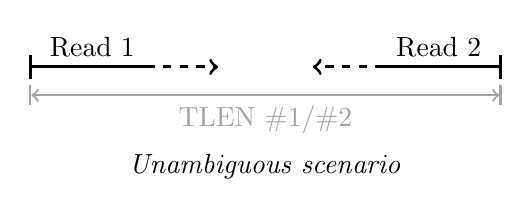
\begin{tikzpicture}[
    thick, xscale=2, yscale=1.8,
    read/.style={line width=0.4mm},
]
\draw[|-, read] (0,0)   -- (0.8,0)  node[midway, above] {Read 1};
\draw[->, read, dashed] (0.85,0) -- (1.2,0);
\draw[|-, read] (3,0) -- (2.2,0) node[midway, above] {Read 2};
\draw[->, read, dashed] (2.25,0) -- (1.8,0);
\draw[|<->|,gray!120]     (0,-.2) -- +(3,0) node[midway, below] {TLEN \#1/\#2};
\node at (1.5,-0.7) {\textit{Unambiguous scenario}};
\end{tikzpicture}
\hspace{3cm}% No space means side by side
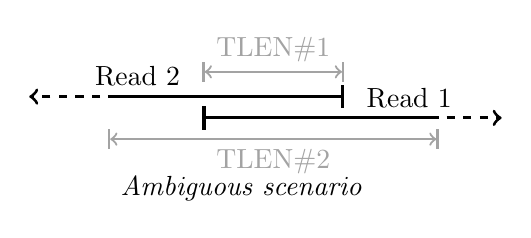
\begin{tikzpicture}[
    thick, xscale=1,yscale=0.9,
    read/.style={line width=0.4mm},
]
\draw[|-, read]         (2.2,0)   -- (5.2,0)    node[very near end, above] {Read 1};
\draw[->, read, dashed] (5.3,0)   -- (6,0);
\draw[-|, read]         (1,.3)    -- (4,.3)     node[very near start , above] {Read 2};
\draw[->, read, dashed] (0.9,.3)  -- (0,.3);
\draw[|<->|,gray!120]   (1,-0.3)  -- (5.2,-0.3) node[midway, below] {TLEN\#2};
\draw[|<->|,gray!120]   (2.2,0.65)-- (4,0.65)    node[midway, above] {TLEN\#1};
\node at (2.7,-1) {\textit{Ambiguous scenario}};
\end{tikzpicture}
\end{center}
}

\item {\sf SEQ}: segment SEQuence. This field can be a `*' when the
  sequence is not stored. If not a `*', the length of the sequence must
  equal the sum of lengths of {\tt M/I/S/=/X} operations in {\sf CIGAR}.
  An `=' denotes the base is identical to the reference base. No
  assumptions can be made on the letter cases.
\item {\sf QUAL}: ASCII of base QUALity plus 33 (same as the quality
  string in the Sanger FASTQ format). A base quality is the phred-scaled
  base error probability which equals $-10\log_{10}\Pr\{\mbox{base is
    wrong}\}$. This field can be a `*' when quality is not stored. If
  not a `*', {\sf SEQ} must not be a `*' and the length of the quality string
  ought to equal the length of {\sf SEQ}.
\end{enumerate}

\subsection{The alignment section: optional fields}\label{sec:alnaux}
All optional fields follow the {\tt TAG:TYPE:VALUE} format
where {\tt TAG} is a two-character string that matches {\tt /[A-Za-z][A-Za-z0-9]/}.
Each {\tt TAG} can only appear once in one alignment line. A {\tt TAG}
containing lowercase letters are reserved for end users.
In an optional field, {\tt TYPE} is a single case-sensitive letter which
defines the format of {\tt VALUE}:
\begin{center}\small
\begin{tabular}{cll}
\hline
{\bf Type} & {\bf Regexp matching {\tt VALUE}} & {\bf Description} \\
\hline
A & {\tt [!-\char126]} & Printable character \\
i & {\tt [-+]?[0-9]+} & Signed integer\footnotemark\\
f & {\tt [-+]?[0-9]*\char92.?[0-9]+([eE][-+]?[0-9]+)?} & Single-precision floating number \\
Z & {\tt [\,\,\,!-\char126]*} & Printable string, including space\\
H & {\tt ([0-9A-F][0-9A-F])*} & Byte array in the Hex format\footnotemark\\
B & {\tt [cCsSiIf](,[-+]?[0-9]*\char92.?[0-9]+([eE][-+]?[0-9]+)?)*} & Integer or numeric array\\
\hline
\end{tabular}
\addtocounter{footnote}{-1}
\footnotetext{The number of digits in an integer optional field is not
explicitly limited in SAM.  However, BAM can represent values in the
range~$[-2^{31},2^{32})$, so in practice this is the realistic range
of values for SAM's `{\tt i}' as well.}
\stepcounter{footnote}
\footnotetext{For example, the six-character Hex string `{\tt 1AE301}' represents the byte array $[{\tt 0x1a},{\tt 0xe3},{\tt 0x1}]$.}
\end{center}
For an integer or numeric array (type `{\tt B}'), the first letter indicates the type of numbers
in the following comma separated array. The letter can be one of `{\tt cCsSiIf}', corresponding to
{\tt int8\_t} (signed 8-bit integer), {\tt uint8\_t} (unsigned 8-bit integer), {\tt int16\_t}, {\tt uint16\_t}, {\tt int32\_t}, {\tt uint32\_t}
and {\tt float}, respectively.\footnotemark\@ During import/export, the element type
may be changed if the new type is also compatible with the array.
\footnotetext{Explicit typing eases format parsing and helps to reduce the file size when SAM is converted to BAM.}

Predefined tags are described in the separate {\sl Sequence Alignment/Map
Optional Fields Specification}.\footnote{See
\href{http://samtools.github.io/hts-specs/SAMtags.pdf}{\tt SAMtags.pdf}
at \url{https://github.com/samtools/hts-specs}.}
See that document for details of existing standard tag fields and conventions
around creating new tags that may be of general interest.
Tags starting with `{\tt X}', `{\tt Y}' or `{\tt Z}' and tags containing
lowercase letters in either position are reserved for local use and will
not be formally defined in any future version of these specifications.

\pagebreak

\section{Recommended Practice for the SAM Format}
\label{sec:recommended-practice}
This section describes the best practice for representing data in the
SAM format. They are not required in general, but may be required by a
specific software package for it to function properly.

\begin{enumerate}
\item The header section
  \begin{enumerate}[label=\arabic*]
  \item The {\tt @HD} line should be present, with either the {\tt SO} tag
    or the {\tt GO} tag (but not both) specified.
  \item The {\tt @SQ} lines should be present if reads have been mapped.
  \item When a {\tt RG} tag appears anywhere in the alignment section,
    there should be a single corresponding {\tt @RG} line with matching
    {\tt ID} tag in the header.
  \item When a {\tt PG} tag appears anywhere in the alignment section,
    there should be a single corresponding {\tt @PG} line with matching
    {\tt ID} tag in the header.
  \end{enumerate}
\item Adjacent CIGAR operations should be different.
\item No alignments should be assigned mapping quality 255.
\item Unmapped reads
  \begin{enumerate}[label=\arabic*]
  \item For a unmapped paired-end or mate-pair read whose mate is
    mapped, the unmapped read should have {\sf RNAME} and {\sf POS}
    identical to its mate.
  \item If all segments in a template are unmapped, their {\sf RNAME}
    should be set as `*' and {\sf POS} as 0.
  \item If {\sf POS} plus the sum of lengths of {\tt M/=/X/D/N}
    operations in {\sf CIGAR} exceeds the length specified in the {\tt
      LN} field of the {\tt @SQ} header line (if exists) with an SN
    equal to {\sf RNAME}, the alignment should be unmapped, unless the
    reference sequence is circular (see below).
  \item Unmapped reads should be stored in the orientation in which they came
    off the sequencing machine and have their {\sf reverse} flag bit~(0x10)
    correspondingly unset.
  \end{enumerate}
\item Multiple mapping
  \begin{enumerate}[label=\arabic*]
  \item When one segment is present in multiple lines to represent a multiple
	mapping of the segment, only one of these records should have the secondary
	alignment flag bit (0x100) unset. {\sf RNEXT} and {\sf PNEXT} point to the
	primary line of the next read in the template.
  \item {\sf SEQ} and {\sf QUAL} of secondary alignments should be set
    to `*' to reduce the file size.
  \end{enumerate}
%\item There should be no overlap between segments of a read\footnote{Few/no
%  existing aligners follow this practice.}.
\item Optional tags:
  \begin{enumerate}[label=\arabic*]
  \item If the template has more than 2 segments, the {\tt TC} tag
    should be present.
  \item The {\tt NM} tag should be present.
  \end{enumerate}

\item Circular reference sequences

Mappings that cross the coordinate `join' in circular reference sequences (i.e., those whose {\tt @SQ} headers specify {\tt TP:circular}) may be represented as follows:
  \begin{enumerate}[label=\arabic*]
  \item (Preferred)
As usual {\sf POS} should be between 1 and the {\tt @SQ} header's {\tt LN} value, but {\sf POS} plus the sum of the lengths of {\tt M/=/X/D/N} {\sf CIGAR} operations may exceed {\tt LN}.
Coordinates greater than~{\tt LN} are interpreted by subtracting {\tt LN} so that bases at $\texttt{LN}+1, \texttt{LN}+2, \texttt{LN}+3, \ldots$ are considered to be mapped at positions $1,2,3,\ldots$; thus each (1-based) position $p$ is interpreted as $((p-1)\bmod\texttt{LN})+1$.%
\footnote{The impact of this representation on indexing and random access is yet to be explored by implementations.}

  \item
Alternatively, such alignments may be split across several records: one record representing the initial portion of the segment ending at~{\tt LN}, one representing the final portion starting from~1, and any other records representing additional portions in between spanning the entire reference sequence.
One record (chosen arbitrarily) is considered primary and the remainder have their {\sf supplementary} flag bit (0x800) set.
  \end{enumerate}

\item Annotation dummy reads:
  These have {\sf SEQ} set to {\tt *}, {\sf FLAG} bits 0x100 and 0x200
  set (secondary and filtered), and a {\tt CT} tag.
  \begin{enumerate}[label=\arabic*]
%Repeating what is in the tag's footnote:
%  \item If the {\tt CT} tag's \emph{strand} is {\tt -}, FLAG bit 0x10
%  (reverse complemented) should be set, and otherwise not set.
  \item If you wish to store free text in a {\tt CT} tag, use the
  \emph{key} value {\tt Note} (uppercase N) to match GFF3.
  \item Multi-segment annotation (e.g., a gene with introns) should be
  described with multiple lines in SAM (like a multi-segment read).
  Where there is a clear biological direction (e.g., a gene), the first
  segment ({\sf FLAG} bit 0x40) is used for the first section (e.g., the
  $5'$ end of the gene). Thus a GenBank entry location like
  {\tt complement(join(85052..85354, 85441..85621, 86097..86284))}
  would have three lines in SAM with a common {\sf QNAME}: %And three lines in GFF3 too.
    \begin{center}\begin{tabular}{llrcl}
  & \multicolumn{1}{c}{\sf FLAG} & \multicolumn{1}{c}{\sf POS} & \sf CIGAR & \multicolumn{1}{c}{Optional fields} \\
The $5'$ fragment & 883 (0x373) & 86097 & \tt 188M & \tt FI:i:1\quad TC:i:3 \\
Middle fragment   & 819 (0x333) & 85441 & \tt 181M & \tt FI:i:2\quad TC:i:3 \\
The $3'$ fragment & 947 (0x3B3) & 85052 & \tt 303M & \tt FI:i:3\quad TC:i:3
    \end{tabular}\end{center}
  \item If converting GFF3 to SAM, store any \emph{key}, \emph{values}
  from column 9 in the {\tt CT} tag, except for the unique ID which
  is used for the QNAME. GFF3 columns 1 (seqid), 4 (start) and 5 (end)
  are encoded using SAM columns RNAME, POS and CIGAR to hold the length.
  GFF3 columns 3 (type) and 7 (strand) are stored explicitly in the
  {\tt CT} tag. Remaining GFF3 columns 2 (source), 6 (score), and
  8 (phase) are stored in the {\tt CT} tag using \emph{key} values
  {\tt FSource}, {\tt FScore} and {\tt FPhase} (uppercase keys are
  restricted in GFF3, so these names avoid clashes). Split location
  features are described with multiple lines in GFF3, and similarly
  become multi-segment dummy reads in SAM, with the {\sf RNEXT} and
  {\sf PNEXT} columns filled in appropriately. In the absence of a
  convention in SAM/BAM for reads wrapping the origin of a circular
  genome, any GFF3 feature line wrapping the origin must be split into
  two segments in SAM.
  \end{enumerate}
\end{enumerate}

\section{Guide for Describing Assembly Sequences in SAM}

\subsection{Unpadded versus padded representation}

To describe alignments, we can regard the reference sequence with no respect to
other alignments against it.  Such a reference sequence is called an
\emph{unpadded reference}. A position on an unpadded reference, referred to
as an \emph{unpadded position}, is not affected by any alignments. When we use
unpadded references and positions to describe alignments, we say we are using
the \emph{unpadded representation}.

Alternatively, to describe the same alignments, we can modify the reference
sequence to contain pads that make room for sequences inserted relative to the
reference. A pad is effectively a gap and conventionally represented by an
asterisk `*'.  A reference sequence containing pads is called a \emph{padded
reference}. A position which counts the *'s is referred to as a \emph{padded
position}. A padded reference sequence may be affected by the query alignments
and because of gap insertions is typically longer than the unpadded reference.
The padded position of one query alignment may be affected by other query
alignments.

Unpadded and padded are different representations of the same alignments. They
are convertible to each other with no loss of any information. The unpadded
representation is more common due to the convenience of a fixed coordinate system,
while the padded representation has the advantage that alignments can be simply
described by the start and end coordinates without using complex CIGAR strings.
SAM traditionally uses the padded representation for {\it de novo} assembly.
The ACE assembly format uses the padded representation exclusively.

\subsection{Padded SAM}\label{sec:padded-sam}

The SAM format is typically used to describe alignments against an unpadded
reference sequence, but it is also able to describe alignments against a padded
reference. In the latter case, we say we are using a \emph{padded SAM}. A padded
SAM is a valid SAM, but with the difference that the reference and positions in
use are padded. There may be more than one way to describe the padded
representation.
We recommend the following; see also the discussion in Cock {\it et al.}%
\footnote{Peter J. A. Cock, James K. Bonfield, Bastien Chevreux, and Heng Li,
{\bf SAM/BAM format v1.5 extensions for \emph{de novo} assemblies},
{\sl bioRxiv 020024};
\href{http://dx.doi.org/10.1101/020024}{doi:10.1101/020024}.}

In a padded SAM, alignments and coordinates are described with respect to the
padded reference sequence. Unlike traditional padded representations like
the ACE file format where pads/gaps are recorded in reads using *'s, we do
not write *'s in the {\sf SEQ} field of the SAM format.\footnote{Writing
pads/gaps as *'s in the {\sf SEQ} field might have been more convenient, but
this caused concerns for backward compatibility.} Instead, we describe pads
in the query sequences as deletions from the padded reference using the
{\sf CIGAR} `{\tt D}' operation. In a padded SAM, the insertion and padding
CIGAR operations (`{\tt I}' and `{\tt P}') are not used because the padded
reference already considers all the insertions.

The following shows the padded SAM for the example alignment in Section~\ref{sec:example}.
Notably, the length of {\tt ref} is 47 instead of 45. {\sf POS} of the last
three alignments are all shifted by 2. {\sf CIGAR} of alignments bridging the
2bp insertion are also changed.

\begin{framed}\small
\begin{verbatim}
@HD VN:1.6 SO:coordinate
@SQ SN:ref LN:47
ref   516 ref  1  0 14M2D31M   *  0   0 AGCATGTTAGATAAGATAGCTGTGCTAGTAGGCAGTCAGCGCCAT *
r001   99 ref  7 30 14M1D3M    = 39  41 TTAGATAAAGGATACTG *
*     768 ref  8 30 1M         *  0   0 *                 * CT:Z:.;Warning;Note=Ref wrong?
r002    0 ref  9 30 3S6M1D5M   *  0   0 AAAAGATAAGGATA    * PT:Z:1;4;+;homopolymer
r003    0 ref  9 30 5H6M       *  0   0 AGCTAA            * NM:i:1
r004    0 ref 18 30 6M14N5M    *  0   0 ATAGCTTCAGC       *
r003 2064 ref 31 30 6H5M       *  0   0 TAGGC             * NM:i:0
r001  147 ref 39 30 9M         =  7 -41 CAGCGGCAT         * NM:i:1
\end{verbatim}
\end{framed}

Here we also exemplify the recommended practice for storing the reference
sequence and the reference annotations in SAM when necessary. For a reference
sequence in SAM, {\sf QNAME} should be identical to {\sf RNAME}, {\sf POS} set
to 1 and {\sf FLAG} to 516 (filtered and unmapped); for an annotation, {\sf
FLAG} should be set to 768 (filtered and secondary) with no restriction to {\sf
QNAME}.
Dummy reads for annotation would typically have a {\tt CT} tag to hold the annotation information; see the discussion of dummy reads in Section~\ref{sec:recommended-practice}.
See also the separate {\sl Optional Fields Specification} for full details of the {\tt CT} and {\tt PT} annotation tags.%
\footnote{See \emph{Annotation and Padding} in \href{http://samtools.github.io/hts-specs/SAMtags.pdf}{\tt SAMtags.pdf}.}

\pagebreak

\section{The BAM Format Specification}

\subsection{The BGZF compression format}

BGZF is block compression implemented on top of the standard gzip file
format.\footnote{L.~Peter Deutsch, {\bf GZIP file format specification
version~4.3}, \href{http://tools.ietf.org/html/rfc1952}{\sl RFC 1952}.}
The goal of BGZF is to provide good compression while allowing
efficient random access to the BAM file for indexed queries. The BGZF
format is `gunzip compatible', in the sense that a compliant gunzip
utility can decompress a BGZF compressed file.\footnote{It is worth noting that there is a known bug in the Java {\sf
  GZIPInputStream} class that concatenated gzip archives cannot be
successfully decompressed by this class. BGZF files can be created and
manipulated using the built-in Java {\sf util.zip} package, but naive
use of {\sf GZIPInputStream} on a BGZF file will not work due to this
bug.}

A BGZF file is a series of concatenated BGZF blocks, each no larger
than~64Kb before or after compression. Each BGZF block
is itself a spec-compliant gzip archive which contains an ``extra field''
in the format described in RFC1952. The gzip file format allows the
inclusion of application-specific extra fields and these are ignored by
compliant decompression implementation. The gzip specification also
allows gzip files to be concatenated. The result of decompressing
concatenated gzip files is the concatenation of the uncompressed data.

Each BGZF block contains a standard gzip file header with the following
standard-compliant extensions:

\begin{enumerate}
\item The {\sf F.EXTRA} bit in the header is set to indicate that extra
  fields are present.
\item The extra field used by BGZF uses the two subfield ID values 66 and 67 (ascii `BC').
\item The length of the BGZF extra field payload (field {\sf LEN} in the
  gzip specification) is 2 (two bytes of payload).
\item The payload of the BGZF extra field is a 16-bit unsigned integer
  in little endian format. This integer gives the size of the containing
  BGZF block minus one.
\end{enumerate}

On disk, a complete BGZF file is a series of blocks as shown in the following
table.  (All integers are little endian as is required by RFC1952.)
\begin{table}[ht]
\centering
{\small
\begin{tabular}{|l|l|l|l|l|r|}
  \cline{1-6}
  \multicolumn{3}{|c|}{\bf Field} & \multicolumn{1}{c|}{\bf Description} & \multicolumn{1}{c|}{\bf Type} & \multicolumn{1}{c|}{\bf Value} \\\cline{1-6}
  \multicolumn{6}{|c|}{\textcolor{gray}{\it List of compression blocks (until the end of the file)}} \\\cline{2-6}
  & \multicolumn{2}{l|}{\sf ID1} & gzip IDentifier1 & {\tt uint8\_t} & 31 \\\cline{2-6}
  & \multicolumn{2}{l|}{\sf ID2} & gzip IDentifier2 & {\tt uint8\_t} & 139 \\\cline{2-6}
  & \multicolumn{2}{l|}{\sf CM} & gzip Compression Method & {\tt uint8\_t} & 8 \\\cline{2-6}
  & \multicolumn{2}{l|}{\sf FLG} & gzip FLaGs & {\tt uint8\_t} & 4 \\\cline{2-6}
  & \multicolumn{2}{l|}{\sf MTIME} & gzip Modification TIME & {\tt uint32\_t} & \\\cline{2-6}
  & \multicolumn{2}{l|}{\sf XFL} & gzip eXtra FLags & {\tt uint8\_t} & \\\cline{2-6}
  & \multicolumn{2}{l|}{\sf OS} & gzip Operating System & {\tt uint8\_t} & \\\cline{2-6}
  & \multicolumn{2}{l|}{\sf XLEN} & gzip eXtra LENgth & {\tt uint16\_t} & \\\cline{2-6}
  & \multicolumn{5}{c|}{\textcolor{gray}{\it Extra subfield(s) (total size=XLEN)}} \\\cline{3-6}
  & & \multicolumn{4}{c|}{\textcolor{gray}{\it Additional RFC1952 extra subfields if present}} \\\cline{3-6}
  & & {\sf SI1} & Subfield Identifier1 & {\tt uint8\_t} & 66 \\\cline{3-6}
  & & {\sf SI2} & Subfield Identifier2 & {\tt uint8\_t} & 67 \\\cline{3-6}
  & & {\sf SLEN} & Subfield LENgth & {\tt uint16\_t} & 2 \\\cline{3-6}
  & & {\sf BSIZE} & total Block SIZE minus 1 & {\tt uint16\_t} & \\\cline{3-6}
  & & \multicolumn{4}{c|}{\textcolor{gray}{\it Additional RFC1952 extra subfields if present}} \\\cline{2-6}
  & \multicolumn{2}{l|}{\sf CDATA} & Compressed DATA by {\sf zlib::deflate()} & {\tt uint8\_t[{\sf BSIZE-XLEN-19}]} & \\\cline{2-6}
  & \multicolumn{2}{l|}{\sf CRC32} & CRC-32 & {\tt uint32\_t} & \\\cline{2-6}
  & \multicolumn{2}{l|}{\sf ISIZE} & Input SIZE (length of uncompressed data) & {\tt uint32\_t} & \\
  \cline{1-6}
\end{tabular}}
\end{table}

The random access method to be described next limits the uncompressed
contents of each BGZF block to a maximum of $2^{16}$~bytes of data.
Thus while {\sf ISIZE} is stored as a {\tt uint32\_t} as per the gzip format,
in BGZF it is limited to the range~$[0,65536]$.
{\sf BSIZE} can represent BGZF block sizes in the range~$[1,65536]$, though
typically {\sf BSIZE} will be rather less than~{\sf ISIZE} due to compression.

\subsubsection{Random access}

BGZF files support random access through the BAM file index. To achieve
this, the BAM file index uses \emph{virtual file offsets} into the BGZF
file. Each virtual file offset is an unsigned 64-bit integer, defined as: {\tt
  coffset\char60\char60 16\char124uoffset}, where {\tt coffset} is an
unsigned byte offset into the BGZF file to the beginning of a BGZF
block, and {\tt uoffset} is an unsigned byte offset into the
uncompressed data stream represented by that BGZF block. Virtual file
offsets can be compared, but subtraction between virtual file offsets
and addition between a virtual offset and an integer are both
disallowed.

\subsubsection{End-of-file marker}

An end-of-file (EOF) trailer or marker block should be written at the end
of BGZF files, so that unintended file truncation can be easily detected.
The EOF marker block is a particular empty\footnotemark\ BGZF block
encoded with the default {\sf zlib} compression level settings,
and consists of the following 28~hexadecimal bytes:
\begin{center}
\texttt{1f 8b 08 04 00 00 00 00 00 ff 06 00 42 43 02 00 1b 00 03 00 00 00 00 00 00 00 00 00}
\end{center}

\footnotetext{Empty in the sense of having been formed by compressing
a data block of length zero.}

\noindent
The presence of this EOF marker at the end of a BGZF file indicates that the
immediately following physical EOF is the end of the file as intended by the
program that wrote it.
Empty BGZF blocks are not otherwise special; in particular, the presence of
an EOF marker block does not by itself signal end of file.\footnotemark

\footnotetext{An implementation that supports reopening a BAM file in append
mode could produce a file by writing headers and alignment records to it,
closing it (adding an EOF marker); then reopening it for append, writing
more alignment records, and closing it (adding an EOF marker).
The resulting BAM file would contain an embedded insignificant EOF~marker
block that should be effectively ignored when it is read.}

The absence of this final EOF marker should trigger a warning or error
soon after opening a BGZF file where random access is available.\footnotemark\
When reading a BGZF file in sequential streaming fashion, ideally this
EOF check should be performed when the end of the stream is reached.
Checking that the final BGZF block in the file decompresses to empty
or checking that the last 28 bytes of the file are exactly the bytes
above are both sufficient tests; each is likely more convenient in
different circumstances.

\footnotetext{It is useful to produce a diagnostic at the beginning of
reading a file, so that interactive users can abort lengthy analysis of
potentially-corrupted files.  Of course, this is only possible if the
stream in question supports random access.}

\pagebreak

\subsection{The BAM format}
BAM is compressed in the BGZF format. All multi-byte numbers in BAM are
little-endian, regardless of the machine endianness. The format is
formally described in the following table where values in brackets are
the default when the corresponding information is not available; an
underlined word in uppercase denotes a field in the SAM format.

\begin{table}[ht]
\centering
{\small
\begin{tabular}{|l|l|l|p{8.15cm}|l|r|}
  \cline{1-6}
  \multicolumn{3}{|c|}{\bf Field} & \multicolumn{1}{c|}{\bf Description} & \multicolumn{1}{c|}{\bf Type} & \multicolumn{1}{c|}{\bf Value} \\\cline{1-6}
  \multicolumn{3}{|l|}{\sf magic} & BAM magic string & {\tt char[4]} & {\tt BAM\char92 1}\\\cline{1-6}
  \multicolumn{3}{|l|}{\sf l\_text} & Length of the header text, including any {\tt NUL} padding & {\tt uint32\_t} & $< 2^{31}$ \\\cline{1-6}
  \multicolumn{3}{|l|}{\sf text} & Plain header text in SAM; not necessarily {\tt NUL}-terminated & {\tt char[{\sf l\_text}]} & \\\cline{1-6}
  % Pedantically this should be <= but we restrict |refs| by one so n_ref fits in a signed 32-bit int.
  \multicolumn{3}{|l|}{\sf n\_ref} & \# reference sequences & {\tt uint32\_t} & $< 2^{31}$ \\\cline{1-6}
  \multicolumn{6}{|c|}{\textcolor{gray}{\it List of reference information (n=n\_ref)}} \\\cline{2-6}
  & \multicolumn{2}{l|}{\sf l\_name} & Length of the reference name plus 1 (including {\tt NUL}) & {\tt uint32\_t} & \memlimited \\\cline{2-6}
  & \multicolumn{2}{l|}{\sf name} & Reference sequence name; {\tt NUL}-terminated & {\tt char[{\sf l\_name}]} & \\\cline{2-6}
  & \multicolumn{2}{l|}{\sf l\_ref} & Length of the reference sequence & {\tt uint32\_t} & $< 2^{31}$ \\\cline{1-6}
  \multicolumn{6}{|c|}{\textcolor{gray}{\it List of alignments (until the end of the file)}} \\\cline{2-6}
  & \multicolumn{2}{l|}{\sf block\_size} & Total length of the alignment record, excluding this field & {\tt uint32\_t} & \memlimited \\\cline{2-6}
  & \multicolumn{2}{l|}{\sf refID} & Reference sequence ID, $-1\leq{\sf refID}<{\sf n\_ref}$; -1 for a read without a mapping position & {\tt int32\_t} & [-1] \\\cline{2-6}
  & \multicolumn{2}{l|}{\sf pos} & 0-based leftmost coordinate ($=\underline{\sf POS}-1$)& {\tt int32\_t} & [-1]\\\cline{2-6}
  & \multicolumn{2}{l|}{\sf l\_read\_name} & Length of {\sf read\_name} below ($={\sf length}(\underline{\sf QNAME})+1$) & {\tt uint8\_t} & \\\cline{2-6}
  & \multicolumn{2}{l|}{\sf mapq} & Mapping quality (=\underline{\sf MAPQ}) & {\tt uint8\_t} & \\\cline{2-6}
  & \multicolumn{2}{l|}{\sf bin} & BAI index bin, see Section~\ref{sec:bin-field}  & {\tt uint16\_t} & \\\cline{2-6}
  & \multicolumn{2}{l|}{\sf n\_cigar\_op} & Number of operations in \underline{\sf CIGAR}, see Section~\ref{sec:ncigar} & {\tt uint16\_t} & \\\cline{2-6}
  & \multicolumn{2}{l|}{\sf flag} & Bitwise flags (= \underline{\sf FLAG})\footnotemark\ & {\tt uint16\_t} & \\\cline{2-6}
  & \multicolumn{2}{l|}{\sf l\_seq} & Length of \underline{\sf SEQ} & {\tt uint32\_t} & \memlimited \\\cline{2-6}
  & \multicolumn{2}{l|}{\sf next\_refID} & Ref-ID of the next segment ($-1\le{\sf next\_refID}<{\sf n\_ref}$) & {\tt int32\_t} & [-1] \\\cline{2-6}
  & \multicolumn{2}{l|}{\sf next\_pos} & 0-based leftmost pos of the next segment ($=\underline{\sf PNEXT}-1$) & {\tt int32\_t} & [-1] \\\cline{2-6}
  & \multicolumn{2}{l|}{\sf tlen} & Template length ($=\underline{\sf TLEN}$) & {\tt int32\_t} & [0] \\\cline{2-6}
  & \multicolumn{2}{l|}{\sf read\_name} & Read name, {\tt NUL}-terminated (\underline{\sf QNAME} with trailing `{\tt\verb"\0"}')\footnotemark & {\tt char[{\sf l\_read\_name}]} & \\\cline{2-6}
  & \multicolumn{2}{l|}{\sf cigar} & CIGAR: {\tt {\sf op\_len}\char60\char60 4\char124{\sf op}}. `{\tt MIDNSHP\char61X}'$\to$`012345678' & {\tt uint32\_t[{\sf n\_cigar\_op}]} & \\\cline{2-6}
  & \multicolumn{2}{l|}{\sf seq} & 4-bit encoded read: `{\tt =ACMGRSVTWYHKDBN}'$\to[0,15]$. See Section~\ref{sec:seq} & {\tt uint8\_t[({\sf l\_seq}+1)/2]} & \\\cline{2-6}
  & \multicolumn{2}{l|}{\sf qual} & Phred-scaled base qualities. See Section~\ref{sec:seq} & {\tt char[{\sf l\_seq}]} & \\\cline{2-6}
  & \multicolumn{5}{c|}{\textcolor{gray}{\it List of auxiliary data (until the end of the alignment block)}} \\\cline{3-6}
  & & {\sf tag} & Two-character tag & {\tt char[2]} & \\\cline{3-6}
  & & {\sf val\_type} & Value type: {\tt AcCsSiIfZHB}, see Section~\ref{sec:aux-type-codes} & {\tt char} & \\\cline{3-6}
  & & {\sf value} & Tag value & (by {\sf val\_type}) &\\
  \cline{1-6}
\end{tabular}}
\end{table}
\addtocounter{footnote}{-1}
\footnotetext{As noted in Section~\ref{sec:alnrecord}, reserved {\sf FLAG} bits
should be written as zero and ignored on reading by current software.}
\stepcounter{footnote}
\footnotetext{For backward compatibility, an absent {\sf QNAME} (represented as `{\tt *}' in SAM) is stored as a C string {\tt "*\char92 0"}.}

\noindent
Most length and count fields described as {\tt uint32\_t} have additional constraints on their range:
$\mbox{\sf l\_text} < 2^{31}$ due to implementation limits;
$\mbox{\sf n\_ref} < 2^{31}$ because {\sf refID} and {\sf next\_refID} are signed;
$\mbox{\sf l\_ref} < 2^{31}$ because {\sf tlen} is signed;
those marked ``\textit{limited}'' are limited by available memory and the practical size of the data represented well before they are limited by, e.g., Java's signed 32-bit integer maximum array size.

\subsubsection{BIN field calculation}\label{sec:bin-field}
{\sf BIN} is calculated using the {\sf reg2bin()} function in
Section~\ref{sec:code}.
For mapped reads this uses $\mbox{\sf POS}-1$ (i.e.,~0-based left position) and the
alignment end point using the alignment length from the {\sf CIGAR} string.
For unmapped reads (e.g.,~paired-end reads where only one part is mapped, see
Section~\ref{sec:recommended-practice}) and reads whose {\sf CIGAR} strings
consume no reference bases at all, the alignment is treated as
being of length one.
Note unmapped reads with {\sf POS} $0$ (which becomes $-1$ in BAM) therefore
use $\mbox{\sf reg2bin}(-1, 0)$ which is computed as $4680$.

\subsubsection{N\_CIGAR\_OP field}\label{sec:ncigar}
With 16 bits, {\sf n\_cigar\_op} can keep at most 65535 CIGAR
operations in BAM files. For an alignment with more CIGAR operations, BAM
stores the real {\sf CIGAR}, encoded the same way as the {\sf cigar} field in
BAM, in the {\tt CG} optional tag of type `{\tt B,I}', and sets {\sf CIGAR} to
`\textit{k}{\tt S}\textit{m}{\tt N}' as a placeholder, where `\textit{k}' equals {\sf l\_seq}, `\textit{m}'
is the reference sequence length in the alignment, and `{\tt S}' and `{\tt N}'
are the soft-clipping and reference-clip CIGAR operators, respectively---i.e.,
in the binary form, {\sf n\_cigar\_op}=2 and {\sf cigar}={\tt [\textit{k}\char60\char60
4\char124{4},\textit{m}\char60\char60 4\char124{3}]}. If tag {\tt CG} is present and
the first CIGAR operation clips the entire read, a BAM parsing library is
expected to update {\sf n\_cigar\_op} and {\sf cigar} with the real CIGAR
stored in the {\tt CG} tag and remove the now-redundant {\tt CG} tag.

\subsubsection{SEQ and QUAL encoding}\label{sec:seq}
Sequence is encoded in 4-bit values, with adjacent bases packed into the same byte starting with the highest 4 bits first.
When {\sf l\_seq} is odd the bottom 4 bits of the last byte are undefined, but we recommend writing these as zero.
The case-insensitive base codes `{\tt =ACMGRSVTWYHKDBN}' are mapped to $[0,15]$ respectively with all other characters mapping to `{\tt N}' (value 15).

Omitted sequence, represented in SAM as `{\tt *}', is represented by {\sf l\_seq} being 0 and {\sf seq} and {\sf qual} zero-length.

Base qualities are stored as bytes in the range $[0,93]$, without any +33 conversion to printable ASCII.
When base qualities are omitted but the sequence is not, {\sf qual} is filled with {\tt 0xFF} bytes (to length {\sf l\_seq}).

\subsubsection{Auxiliary data encoding}\label{sec:aux-type-codes}
Optional alignment fields are stored immediately after each other immediately
following the {\sf qual} field, and are included in {\sf block\_size}.
Each field is represented as a two-character tag followed by a single type
character and then its value, whose length is determined by the field's type.

\newcommand*{\tagfield}[2]{\firstbytebox{2}{\em tag}\bytebox{1}{\tt #1}#2}

Single character `{\tt A}' fields have a total length of 4~bytes,
with the value represented as a single byte:
\begin{center}\small\byteboxsetup
\tagfield{A}{\bytebox{1}{char}}
\end{center}

While all single (i.e., non-array) integer types are stored in SAM as `{\tt i}',
in BAM any of `{\tt cCsSiI}' may be used together with the correspondingly-sized
binary integer value, chosen according to the field value's magnitude.%
\footnote{The signedness and size used for each integer value is an
implementation choice, but is typically the smallest that suffices.}
Similarly floating point `{\tt f}' fields are represented as IEEE 754-2008
binary32 values.
Thus BAM numeric fields have a total length of~4, 5, or~7~bytes:
\begin{center}\small\byteboxsetup\begin{tabular}{l@{\hspace{1in}}l}
\tagfield{c}{\bytebox{1}{i8}} \quad (i.e., {\tt int8\_t})
    & \tagfield{i}{\bytebox{4}{int32\_t}} \\
\tagfield{C}{\bytebox{1}{u8}} \quad (i.e., {\tt uint8\_t})
    & \tagfield{I}{\bytebox{4}{uint32\_t}} \\
\tagfield{s}{\bytebox{2}{int16\_t}}
    & \tagfield{f}{\bytebox{4}{float}} \\
\tagfield{S}{\bytebox{2}{uint16\_t}}
    &
\end{tabular}\end{center}

\newcommand*{\byteboxvector}[2]{\bytebox{#1}{#2}\bytebox{#1}{#2}\makebox[1.5\bytewidth][c]{$\cdots$}\firstbytebox{#1}{#2}}

String fields and hex-formatted byte arrays are represented as
{\tt NUL}-terminated text strings:%
\footnote{The BAM representation of `{\tt H}' field values as textual
hexadecimal digits rather than binary data is for historical reasons.
Modern applications may prefer to use `{\tt B,C}' array fields rather
than `{\tt H}' fields.}
\begin{center}\small\byteboxsetup\begin{tabular}{l}
\tagfield{Z}{\byteboxvector{1}{char}\bytebox{1}{\tt NUL}} \\
\tagfield{H}{\byteboxvector{2}{hex hex}\bytebox{1}{\tt NUL}}
\end{tabular}\end{center}

\newcommand*{\arraytagfield}[3]{\tagfield{B}{\bytebox{1}{\tt #1}\bytebox{4}{\em count}\byteboxvector{#2}{#3}}}

\begin{samepage}
The representation of a `{\tt B}' array field starts with a sub-type character
similar to the numeric field types above and a \emph{count} ({\tt uint32\_t}, but
limited by memory and {\sf block\_size}) giving the number of elements in the array.
The array elements follow, encoded as binary integers or IEEE floats sized
according to the sub-type:
\begin{center}\small\byteboxsetup\begin{tabular}{l}
\arraytagfield{c}{1}{i8} \quad (i.e., {\tt int8\_t} elements) \\
\arraytagfield{C}{1}{u8} \quad (i.e., {\tt uint8\_t} elements) \\
\arraytagfield{s}{2}{int16\_t} \\
\arraytagfield{S}{2}{uint16\_t} \\
\arraytagfield{i}{4}{int32\_t} \\
\arraytagfield{I}{4}{uint32\_t} \\
\arraytagfield{f}{4}{float}
\end{tabular}\end{center}
\end{samepage}

\pagebreak

\section{Indexing BAM}
Indexing aims to achieve fast retrieval of alignments overlapping a
specified region without going through the whole alignments. BAM must be
sorted by the reference ID and then the leftmost coordinate before
indexing.

This section describes the binning scheme underlying coordinate-sorted
BAM indices and its implementation in the long-established BAI format.
The CSI format documented elsewhere uses a similar binning scheme and
can also be used to index BAM.\footnotemark

\footnotetext{See \href{http://samtools.github.io/hts-specs/CSIv1.pdf}
{\tt CSIv1.pdf} at \url{https://github.com/samtools/hts-specs}.
This is a separate specification because CSI is also used to index other
coordinate-sorted file formats in addition to BAM.}

\subsection{Algorithm}
\subsubsection{Basic binning index}
The UCSC binning scheme was suggested by Richard Durbin and Lincoln Stein
and is explained in Kent {\it et al.}\footnotemark\ In this scheme, each bin
represents a contiguous genomic region which is either fully contained
in or non-overlapping with another bin; each alignment is associated
with a bin which represents the smallest region containing the entire
alignment. The binning scheme is essentially a representation of
R-tree. A distinct bin uniquely corresponds to a distinct internal node
in a R-tree. Bin A is a child of Bin B if the region represented by A is
contained in B.

\footnotetext{W.~James Kent {\it et al.},
{\bf The Human Genome Browser at UCSC}, {\sl Genome Res.}~2002~12: 996--1006;
\href{http://dx.doi.org/doi:10.1101/gr.229102}{doi:10.1101/\linebreak[1]gr.229102};
{\sc pmid:}12045153.  See in particular {\sl The Database}, p1003.}

To find the alignments that overlap a specified region, we need to get
the bins that overlap the region, and then test each alignment in the
bins to check overlap. To quickly find alignments associated with a
specified bin, we can keep in the index the start file offsets of chunks
of alignments which all have the bin. As alignments are sorted by the
leftmost coordinates, alignments having the same bin tend to be
clustered together on the disk and therefore usually a bin is only
associated with a few chunks. Traversing all the alignments having the
same bin usually needs a few seek calls. Given the set of bins that
overlap the specified region, we can visit alignments in the order of
their leftmost coordinates and stop seeking the rest when an alignment
falls outside the required region. This strategy saves half of the seek
calls in average.

In the BAI format, each bin may span $2^{29}$, $2^{26}$, $2^{23}$, $2^{20}$,
$2^{17}$ or $2^{14}$ bp. Bin 0 spans a 512Mbp region, bins 1--8 span 64Mbp,
9--72 8Mbp, 73--584 1Mbp, 585--4680 128Kbp, and bins 4681--37448 span 16Kbp
regions.  This implies that this index format does not support reference
chromosome sequences longer than $2^{29}-1$.

The CSI format generalises the sizes of the bins, and supports reference
sequences of the same length as are supported by SAM and BAM.

\subsubsection{Reducing small chunks}
Around the boundary of two adjacent bins, we may see many small chunks
with some having a shorter bin while the rest having a larger bin. To
reduce the number of seek calls, we may join two chunks having the same
bin if they are close to each other. After this process, a joined chunk
will contain alignments with different bins. We need to keep in the
index the file offset of the end of each chunk to identify its
boundaries.

\subsubsection{Combining with linear index}
For an alignment starting beyond 64Mbp, we always need to seek to some
chunks in bin 0, which can be avoided by using a linear index. In the
linear index, for each tiling 16384bp window on the reference, we record
the smallest file offset of the alignments that overlap with the
window. Given a region [rbeg,\,rend), we only need to visit a chunk whose
end file offset is larger than the file offset of the 16kbp window
containing rbeg.

With both binning and linear indices, we can retrieve alignments in most
of regions with just one seek call.

\subsubsection{A conceptual example}
Suppose we have a genome shorter than 144kbp. We can design a binning
scheme which consists of three types of bins: bin 0 spans 0-144kbp, bin
1, 2 and 3 span 48kbp and bins from 4 to 12 span 16kbp each:

\begin{table}[ht]
  \centering
  {\small\begin{tabular}{|c|c|c|c|c|c|c|c|c|}
    \cline{1-9}
    \multicolumn{9}{|c|}{0 (0--144kbp)}\\\cline{1-9}
    \multicolumn{3}{|c|}{1 (0--48kbp)} & \multicolumn{3}{c|}{2 (48--96kbp)} & \multicolumn{3}{c|}{3 (96--144kbp)} \\\cline{1-9}
    4 (0--16k) & 5 (16--32k) & 6 (32--48k) & 7 (48--64k) & 8 (64--80k) & 9 (80--96k) & 10 & 11 & 12 \\
    \cline{1-9}
  \end{tabular}}
\end{table}

An alignment starting at 65kbp and ending at 67kbp would have a bin
number 8, which is the smallest bin containing the alignment. Similarly,
an alignment starting at 51kbp and ending at 70kbp would go to bin 2,
while an alignment between [40k,\,49k] to bin 0. Suppose we want to find
all the alignments overlapping region [65k,\,71k). We first calculate that
bin 0, 2 and 8 overlap with this region and then traverse the alignments
in these bins to find the required alignments. With a binning index
alone, we need to visit the alignment at [40k,\,49k] as it belongs to bin
0. But with a linear index, we know that such an alignment stops before
64kbp and cannot overlap the specified region. A seek call can thus be
saved.

\subsection{The BAI index format for BAM files}
\begin{table}[ht]
\centering\small
\begin{tabular}{|l|l|l|l|l|l|r|}
  \cline{1-7}
  \multicolumn{4}{|c|}{\bf Field} & \multicolumn{1}{c|}{\bf Description} & \multicolumn{1}{c|}{\bf Type} & \multicolumn{1}{c|}{\bf Value} \\\cline{1-7}
  \multicolumn{4}{|l|}{\sf magic} & Magic string & {\tt char[4]} & {\tt BAI\char92 1}\\\cline{1-7}
  \multicolumn{4}{|l|}{\sf n\_ref} & \# reference sequences & {\tt uint32\_t} & $< 2^{31}$ \\\cline{1-7}
  \multicolumn{7}{|c|}{\textcolor{gray}{\it List of indices (n=n\_ref)}} \\\cline{2-7}
  & \multicolumn{3}{l|}{\sf n\_bin} & \# distinct bins (for the binning index) & {\tt uint32\_t} & $\le 37451$ \\\cline{2-7}
  & \multicolumn{6}{c|}{\textcolor{gray}{\it List of distinct bins (n=n\_bin)}} \\\cline{3-7}
  & & \multicolumn{2}{l|}{\sf bin} & Distinct bin & {\tt uint32\_t} & $\le 37450$ \\\cline{3-7}
  & & \multicolumn{2}{l|}{\sf n\_chunk} & \# chunks & {\tt uint32\_t} & \memlimited\footnotemark \\\cline{3-7}
  & & \multicolumn{5}{c|}{\textcolor{gray}{\it List of chunks (n=n\_chunk)}} \\\cline{4-7}
  & & & {\sf chunk\_beg} & (Virtual) file offset of the start of the chunk & {\tt uint64\_t} & \\\cline{4-7}
  & & & {\sf chunk\_end} & (Virtual) file offset of the end of the chunk & {\tt uint64\_t} & \\\cline{2-7}
  & \multicolumn{3}{l|}{\sf n\_intv} & \# 16kbp intervals (for the linear index) & {\tt uint32\_t} & $\le 2^{17}$ \\\cline{2-7}
  & \multicolumn{6}{c|}{\textcolor{gray}{\it List of intervals (n=n\_intv)}} \\\cline{3-7}
  & & \multicolumn{2}{l|}{\sf ioffset} & (Virtual) file offset of the first alignment in the interval & {\tt uint64\_t} & \\\cline{1-7}
  \multicolumn{4}{|l|}{{\sf n\_no\_coor} (optional)} & Number of unplaced unmapped reads ({\sf RNAME} *) & {\tt uint64\_t} & \\\cline{1-7}
\end{tabular}
\end{table}

\footnotetext{The number of chunks in a single bin is effectively limited by available memory and in any case is typically a maximum of some thousands.}

The index file may optionally contain additional metadata providing a summary
of the number of mapped and placed unmapped read-segments per reference sequence,
and of any unplaced unmapped read-segments.\footnote{By \emph{placed unmapped
read} we mean a read that is unmapped according to its {\sf FLAG} but whose
{\sf RNAME} and~{\sf POS} fields are filled in, thus ``placing'' it on a
reference sequence (see Section~\ref{sec:recommended-practice}).
In contrast, \emph{unplaced} unmapped reads have~`*' and~0 for {\sf RNAME}
and~{\sf POS}.}
This is stored in an optional extra metadata pseudo-bin for each reference
sequence, and in the optional trailing {\sf n\_no\_coor} field at the end of
the file.

The pseudo-bins appear in the references' lists of distinct bins as bin
number~37450 (which is beyond the normal range) and are laid out so as to be
compatible with real bins and their chunks:

\begin{table}[ht]
\centering\small
\begin{tabular}{|l|l|l|r|}
  \hline
  {\sf bin} & Magic bin number & {\tt uint32\_t} & 37450 \\\hline
  {\sf n\_chunk} & \# chunks & {\tt uint32\_t} & 2 \\\hline
  {\sf ref\_beg} & (Virtual) file offset of the start of reads placed on this reference& {\tt uint64\_t} & \\\hline
  {\sf ref\_end} & (Virtual) file offset of the end of reads placed on this reference& {\tt uint64\_t} & \\\hline
  {\sf n\_mapped} & Number of mapped read-segments for this reference & {\tt uint64\_t} & \\\hline
  {\sf n\_unmapped} & Number of unmapped read-segments for this reference & {\tt uint64\_t} & \\\hline
\end{tabular}
\end{table}

\noindent
The {\sf ref\_beg}/{\sf ref\_end} fields locate the first and last reads on this reference sequence, whether they are mapped or placed unmapped.
Thus they are equal to the minimum {\sf chunk\_beg} and maximum {\sf chunk\_end} respectively.

\subsection{C source code for computing bin number and overlapping bins}\label{sec:code}
The following functions compute bin numbers and overlaps for a BAI-style
binning scheme with $6$~levels and a minimum bin size of $2^{14}$~bp.
See the CSI specification for generalisations of these functions designed for
binning schemes with arbitrary depth and sizes.

When these functions are called with regions representing unplaced
unmapped reads, e.g., $\mbox{\sf reg2bin}(-1, 0)$, they involve operations
such as \verb|(-1)>>14| which are undefined or implementation-defined in
some programming languages.
They must be implemented as if these operations use the common
two's-complement semantics: $\mbox{\sf reg2bin}(-1, 0) = 4680$ and
$\mbox{\sf reg2bins}(-1, 0, \ldots)$ returns $[\,0, 0, 8, 72, 584, 4680\,]$.

{\small
\begin{verbatim}
/* calculate bin given an alignment covering [beg,end) (zero-based, half-closed-half-open) */
int reg2bin(int beg, int end)
{
    --end;
    if (beg>>14 == end>>14) return ((1<<15)-1)/7 + (beg>>14);
    if (beg>>17 == end>>17) return ((1<<12)-1)/7 + (beg>>17);
    if (beg>>20 == end>>20) return ((1<<9)-1)/7  + (beg>>20);
    if (beg>>23 == end>>23) return ((1<<6)-1)/7  + (beg>>23);
    if (beg>>26 == end>>26) return ((1<<3)-1)/7  + (beg>>26);
    return 0;
}
/* calculate the list of bins that may overlap with region [beg,end) (zero-based) */
#define MAX_BIN (((1<<18)-1)/7)
int reg2bins(int beg, int end, uint16_t list[MAX_BIN])
{
    int i = 0, k;
    --end;
    list[i++] = 0;
    for (k =    1 + (beg>>26); k <=    1 + (end>>26); ++k) list[i++] = k;
    for (k =    9 + (beg>>23); k <=    9 + (end>>23); ++k) list[i++] = k;
    for (k =   73 + (beg>>20); k <=   73 + (end>>20); ++k) list[i++] = k;
    for (k =  585 + (beg>>17); k <=  585 + (end>>17); ++k) list[i++] = k;
    for (k = 4681 + (beg>>14); k <= 4681 + (end>>14); ++k) list[i++] = k;
    return i;
}
\end{verbatim}
}

\pagebreak

\begin{appendices}
\appendix
\section{Parsing region notation}\label{sec:parse-region}

Parsing region notation such as \emph{name}{\tt [:}\emph{begin}{\tt [-}\emph{end}{\tt ]]} (in which omission of the outer bracketed portion indicates a request for the entire reference sequence) would be simple if \emph{name} could not itself contain `{\tt :}' characters, but this is not the case.
(No such notation containing an optional `{\tt :}' appears in the SAM format itself, but various tools use this notation as a convenient way for their users to specify regions of interest.)

The set of valid reference sequence names is usually already known when parsing this notation---for example, because the associated {\tt @SQ} headers have already been encountered.
Tools can use this set to determine unambiguously which colons could delimit a known-valid reference sequence name.

In pseudocode form, a string~\emph{str} can be parsed as follows:

\begin{tabbing}
\qquad\quad
\= consider the rightmost `{\tt :}' character, if any, of \emph{str} \+\\
if \emph{str} is of the form `\emph{prefix}{\tt :NUM}' \= or `\emph{prefix}{\tt :NUM-NUM}' \\
\> or generally `\emph{prefix}{\tt :}\emph{suffix}' for some plausible interval suffix \\
then \\
\qquad \= if both \emph{prefix} and \emph{str} are in the known set then\quad{\sf\ldots error: ambiguous representation} \\
\> else if \emph{prefix} is in the known set then return (\emph{prefix}, {\tt NUM}\ldots{\tt NUM}) \\
\> else if \emph{str} is in the known set then return (\emph{str}, entire sequence) \\
\> else\quad{\sf\ldots error: unknown reference sequence name} \\
\\
else\qquad{\sf\ldots either {\sl str} does not contain a colon or the suffix is not plausibly numeric}
\\
\> if \emph{str} is in the known set then return (\emph{str}, entire sequence) \\
\> else\quad{\sf\ldots error: unknown reference sequence name or invalid interval syntax}
\end{tabbing}

\noindent
The check leading to ``{\sf error: ambiguous representation}'' is important as it prevents confusing interpretations of actually ambiguous input.
Typically the set of valid reference sequence names will not contain names that are prefixes of other names in the set, so in practice this error will not usually be encountered in non-malicious data.

Either in addition to this algorithm or as an alternative to it, tools can use additional delimiter characters to make an unambiguously parsable notation.
We recommend a convention using curly brackets around the reference sequence name--- \verb"{"\emph{name}\verb"}"{\tt [:}\emph{begin}{\tt [-}\emph{end}{\tt ]]} ---as being memorable, easily typed, unambiguous, and not expanded by most shells.
% (RNAME cannot contain commas, so Bash's {a,b} brace expansion won't occur.)

\section{SAM Version History}\label{sec:history}

This lists the date of each tagged SAM version along with changes that
have been made while that version was current.  The key changes
that caused the version number to change are shown in bold.

Additions and changes to the standard predefined tags are listed in the
separate {\sl Sequence Alignment/Map Optional Fields Specification}.%
\footnote{See Appendix~A of
\href{http://samtools.github.io/hts-specs/SAMtags.pdf}{\tt SAMtags.pdf}
at \url{https://github.com/samtools/hts-specs}.}

\subsection*{1.6: 28 November 2017 to current}

\begin{itemize}
\item Bin calculation changed for alignment records whose CIGAR strings consume no reference bases: like unmapped records, they are considered to have length one (rather than zero). (Jan 2021)
\item Correct the description of index pseudo-bins, which previously stated that {\sf ref\_beg}/{\sf ref\_end}, then named {\sf unmapped\_beg}/{\sf unmapped\_end}, include only placed unmapped reads. (Jul 2020)
\item Add {\tt DNBSEQ} to the list of {\tt @RG PL} header tag values. (Apr 2020)
\item Add {\tt @SQ TP} circular/linear topology header tag. (May 2019)
\item\textbf{Restricted the allowable punctuation characters in reference sequence names} (in {\tt @SQ SN}, {\sf RNAME}, etc).
The sets of characters allowed in {\tt @SQ SN} and {\tt @SQ AN} are now identical, which enlarges the previous {\tt AN} set. (Jan 2019)

We recommend that implementations validating reference sequence names do so using the rules in Section~\ref{sec:charset}; are more lenient for files declaring $\mbox{\tt @HD VN} \leq 1.5$; and validate {\tt AN} only against these rules, not the previous more restrictive {\tt AN} rules.

\item Add {\tt @HD SS} sorting details header tag. (Oct 2018)
\item B array optional fields may have no entries---this was already representable in BAM, clarified that empty arrays are permitted in SAM too. (Jul 2018)
\item Add {\tt @SQ DS} header tag. (Jul 2018)
\item Add {\tt @RG BC} header tag. (Apr 2018)
\item Permit UTF-8 in a few header tags. (Mar 2018)
\item\textbf{Add support for CIGAR strings with more than 65,535 operations.} (Nov 2017)
\end{itemize}

\subsection*{1.5: 23 May 2013 to November 2017}

\begin{itemize}
\item Add {\tt @SQ AN} header tag, allowing only alphanumeric and `\verb"*+.@_|-"' characters in its names. (Jul 2017)
\item Add {\tt @SQ AH} header tag. (Mar 2017)
\item Auxiliary tags migrated to SAMtags document. (Sep 2016)
\item Z and H auxiliary tags are permitted to be zero length. (Jun 2016)
\item QNAME limited to 254 bytes (was 255). (Aug 2015)
\item Generalise 0x200 flag bit as filtered-out bit. (Aug 2015)
\item Add {\tt @HD GO} for group order. (Mar 2015)
\item Add {\tt ONT} to the {\tt @RG PL} and {\tt @RG PM} header tags. (Mar 2015)
\item Add meaning to reverse FLAG on unmapped reads. (Mar 2015)
\item Document the {\tt idxstats} .bai elements. (Nov 2014)
\item Addition of CSI index. (Sep 2014)
\item Add {\tt @PG DS} header field. (Dec 2013)
\item Document the BAM EOF byte values. (Dec 2013)
\item Glossary of alignment types. (May 2013)
\item Note that PNEXT/RNEXT points to next read, not segment. (May 2013)
\item \textbf{Add SUPPLEMENTARY flag bit}. (May 2013)
\end{itemize}

\subsection*{1.4: 21 April 2011 to May 2013}

\begin{itemize}
\item Add guide to using sequence annotations ({\tt CT/PT} tags). (Mar 2012)
\item Increase max reference length from $2^{29}$ to $2^{31}$. (Sep
  2011)
\item Clarify {\tt @SQ M5} header tag generation. (Sep 2011)
\item Describe padded alignments. (Sep 2011)
\item Add {\tt @RG FO}, {\tt KS} header fields. (Apr 2011)
\item Clarify chaining of PG records. (Apr 2011)
\item \textbf{Add {\tt B} array auxiliary tag type.} (Apr 2011)\
\item \textbf{Permit IUPAC in SEQ and {\tt MD} auxiliary tag.} (Apr 2011)
\item \textbf{Permit QNAME ``{\tt *}''.} (Apr 2011)
\end{itemize}

\subsection*{1.3: July 2010 to April 2011}

\begin{itemize}
\item Add {\tt RG PG} header field. (Nov 2010)
\item Add BAM description and index sections. (Nov 2010)
\item \textbf{Removal of FLAG letters.} (July 2010)
\item The {\tt SM} header field, previously mandatory for {\tt @RG}, is now
optional. (July 2010)
\end{itemize}

\subsection*{1.0: 2009 to July 2010}

Initial edition.

\end{appendices}
\end{document}
